% Retoca las líneas marcadas con TODO según las necesidades

\documentclass[oneside,a4paper,12pt]{book} % TODO: cambia "oneside" por "twoside" a la hora de imprimirlo

\usepackage[spanish]{babel}
\usepackage[utf8]{inputenc}
\usepackage{geometry}
\usepackage{makeidx}
\usepackage{url}
\usepackage{graphicx}
\usepackage{color}
\usepackage{caption}
\usepackage{acronym}
\usepackage{hyphenat}
\usepackage{a4wide}
\usepackage[normalsize]{subfigure}
\usepackage{float}
\usepackage{titlesec}
\usepackage[Lenny]{fncychap}
\usepackage{listings} % para poder hacer uso de "listings" propios (p.ej. códigos)
\usepackage{eurosym} % para poder usar el símbolo del euro con \euro {xx}
\usepackage{hyperref} % TODO: añade la opción hidelinks para imprimirlo (los enlaces no aparecerán resaltados)
\usepackage[shortlabels]{enumitem}

% Para que no parta las palabras
\pretolerance=10000

\newcommand{\bigrule}{\titlerule[0.5mm]} \titleformat{\chapter}[display] % cambiamos el formato de los capítulos
{\bfseries\Huge} % por defecto se usaron caracteres de tamaño huge en negrita
{% contenido de la etiqueta 
	\titlerule % línea horizontal 
	\filright % texto alineado a la derecha 
	\Large\chaptertitlename\ % capítulo e índice en tamaño large
	\Large % en lugar de 
	\Huge \Large\thechapter}
{0mm} % espacio mínimo entre etiqueta y cuerpo
{\filright} % texto del cuerpo alineado a la derecha
[\vspace{0.5mm} \bigrule] % después del cuerpo, dejar espacio vertical y trazar línea horizontal gruesa
\geometry{a4paper, left=3.5cm, right=2cm, top=3cm, bottom=2cm, headsep=1.5cm}

% Estilos para ilustrar códigos:
\definecolor{code_green}{rgb}{0,0.6,0}
\definecolor{code_gray}{rgb}{0.5,0.5,0.5}
\definecolor{code_mauve}{rgb}{0.58,0,0.82}

\lstset{frame=tb,
	language=C,
	aboveskip=3mm,
	belowskip=3mm,
	showstringspaces=false,
	columns=flexible,
	basicstyle={\small\ttfamily},
	numbers=none,
	numberstyle=\tiny\color{code_gray},
	keywordstyle=\color{blue},
	commentstyle=\color{code_green},
	stringstyle=\color{code_mauve},
	breaklines=true,
	breakatwhitespace=true,
	tabsize=3
}

\lstset{frame=tb,
	language=C++,
	aboveskip=3mm,
	belowskip=3mm,
	showstringspaces=false,
	columns=flexible,
	basicstyle={\small\ttfamily},
	numbers=none,
	numberstyle=\tiny\color{code_gray},
	keywordstyle=\color{blue},
	commentstyle=\color{code_green},
	stringstyle=\color{code_mauve},
	breaklines=true,
	breakatwhitespace=true,
	tabsize=3
}

\lstset{frame=tb,
	language=Python,
	aboveskip=3mm,
	belowskip=3mm,
	showstringspaces=false,
	columns=flexible,
	basicstyle={\small\ttfamily},
	numbers=none,
	numberstyle=\tiny\color{code_gray},
	keywordstyle=\color{blue},
	commentstyle=\color{code_green},
	stringstyle=\color{code_mauve},
	breaklines=true,
	breakatwhitespace=true,
	tabsize=3
}

% Definición de mis propios tipos: Códigos, Ecuaciones y Tablas
\DeclareCaptionType{code}[Código][Listado de códigos]
\DeclareCaptionType{myequation}[Ecuación][Listado de ecuaciones]

% TODO: especifica las reglas de separación que consideres. Algunos ejemplos:
\hyphenation{fuer-tes}
\hyphenation{mul-ti-ca-pa}
\hyphenation{res-pues-ta}
\hyphenation{di-fe-ren-tes}
\hyphenation{de-sa-rro-lla-dos}
\hyphenation{re-pre-sen-tan-do}

 % archivo de configuraci�n de estilo

\makeindex

\begin{document}
\baselineskip 1.35\baselineskip

\frontmatter

\thispagestyle{empty}
\vspace{2cm}

\begin{figure}[htb]
	\centerline{\resizebox{.60\textwidth}{!}{
\includegraphics{figs/logo_urjc}}}
\end{figure}

\begin{center}
	{\Large {\bf GRADO EN INGENIERÍA DE ROBÓTICA SOFTWARE}}
	\vspace{5mm}

	{\large {Escuela Técnica Superior de Ingeniería de Telecomunicación}}
	\vspace{5mm}

	{\large {Curso académico 2021-2022}}

	\vspace{1cm}

	{\large {\bf Trabajo fin de grado}}

	\vspace{2cm}

	{\Large {Conducción autónoma sobre plataforma real y simulada con seguimiento de carril e identificación de señales de tráfico y peatones mediante redes neuronales\\[1cm] }}

	\vspace{5cm}
	{\bf Tutor}: Julio Vega Pérez \\
	{\bf Autor}: Álvaro Mariscal Ávila
\end{center}

\clearpage
\thispagestyle{empty}


% Este diseño se corresponde con la licencia CC-BY-NC-SA.
% Por supuesto, puedes poner la licencia que mejor se adapte al propósito de tu trabajo.
% Recuerda que, si no se especifica ninguna licencia, esta -como cualquier creación artística- pasaría a estar licenciada con todos los derechos reservados (copyright).

\vspace{5cm}

\begin{flushright}

\begin{figure}

\includegraphics[width=0.10\textwidth,right]{figs/by-nc-sa.png}
\end{figure}

\vspace{0.2cm}

{\tiny 
(CC) \textbf{Julio Vega}\\ % TODO: pon aquí tu nombre cuando hagas el documento
\vspace{0.5cm}
\emph{
Este trabajo se entrega bajo licencia \href{https://creativecommons.org/licenses/by-nc-sa/3.0/es/}{CC BY-NC-SA}. \\
Usted es libre de \textit{(a) compartir}: copiar y redistribuir el material en \\
cualquier medio o formato; y \textit{(b) adaptar}: remezclar, transformar \\
y crear a partir del material. El licenciador no puede revocar estas \\
libertades mientras cumpla con los términos de la licencia. \\}
}

\end{flushright}



\cleardoublepage

\chapter*{Agradecimientos}

A mis padres.\\

A mi abuela, aunque ella ya no lo recuerde.\\
\ % Algo de separación...


\

\

\

\

\

\

\

\

\

\

\

\begin{flushright}
		\vspace{4.0 cm}
		\vspace{1.0 cm}
		Madrid, 30 de junio de 2022\\
		\emph{Álvaro Mariscal Ávila}
\end{flushright}

\thispagestyle{empty}


\cleardoublepage

\chapter*{Resumen\markboth{Resumen}{Resumen}}

El problema abordado se enmarca dentro del ámbito de la robótica y la visión artificial. Se trata de dos campos en auge actualmente que proporcionan soluciones eficaces en multitud de campos de aplicación, como por ejemplo, la conducción autónoma, la robótica de inspección o la realidad aumentada.\\

El problema tiene como objetivo desarrollar un coche autónomo sobre una plataforma de bajo coste y reducido tamaño capaz de circular por un circuito o carretera en un entorno dinámico interactuando con objetos propios de una ciudad. El objetivo propuesto se ha desarrollado en dos entornos distintos; en un entorno simulado donde se realizan diversas pruebas con el objetivo de comprobar la viabilidad de la solución planteada, para a continuación, reproducir ese mismo escenario en un entorno real, implementando la solución sobre un robot real.\\

El presente trabajo se ha resuelto a través del uso de dos redes neuronales, una para el seguimiento de carril que se combina con un controlador que utiliza la salida de dicha red para comandar una velocidad lineal y angular u otra al robot. Y otra red neuronal que tiene como objetivo detectar los objetos presentes en el entorno y reaccionar en consecuencia a ellos.\\

Al tratarse de una plataforma de bajo coste, se han encontrado limitaciones propias de la potencia que ofrece el equipo que compone el robot, a pesar de estas dificultades, se ha conseguido resolver el problema propuesto, principalmente reduciendo la resolución de la imagen que reciben las redes neuronales. Además, se han planteado otros ámbitos de aplicación distintos a la conducción autónoma en los que el software desarrollado podría ser aplicado.


\cleardoublepage

\chapter*{Acrónimos\markboth{Acrónimos}{Acrónimos}}

% Añade a continuación los acrónimos que uses en el documento. Algunos ejemplos:
\begin{acronym}
	\acro{AI}{\emph{Artificial Intelligence}}
	\acro{ANN}{\emph{Artificial Neural Network}}
	\acro{AGV}{\emph{Automated Guided Vehicle}}
	\acro{AMR}{\emph{Autonomous Mobile Robot}}
	\acro{CPU}{\emph{Central Processing Unit}}
	\acro{GPU}{\emph{Graphics Processing Unit}}
	\acro{EO/IR}{\emph{Electro-Optical and Infrared Sensors}}
	\acro{FIR}{\emph{Far Infrared}}
	\acro{GPIO}{\emph{General Purpose Input/Output}}
	\acro{RPM}{\emph{Revolutions Per Minute}}
	\acro{PWM}{\emph{Pulse With Modulation}}
	\acro{CW}{\emph{Clockwise}}
	\acro{CCW}{\emph{Counter Clockwise}}
	\acro{LIPO}{\emph{Lithium-Ion Polymer Battery}}
	\acro{USB}{\emph{Universal Serial Bus}}
	\acro{YOLO}{\emph{You Only Look Once}}
	\acro{CNN}{\emph{Convolutional Neural Network}}
	\acro{GUI}{\emph{Graphical User Interface}}
	\acro{MSE}{\emph{Mean Squared Error}}
	\acro{FPS}{\emph{Frames Per Second}}
	\acro{HSV}{\emph{Hue Saturation Value}} 
	\acro{RGB}{\emph{Red Green Blue}}
	\acro{RGBD}{\emph{Red Green Blue Depth}}
	\acro{FP16}{\emph{16-bit Floating Point}}
	\acro{FP32}{\emph{32-bit Floating Point}}
\end{acronym}


\cleardoublepage

\tableofcontents

\listoffigures

\listofcodes

% \listofmyequations

\listoftables

\cleardoublepage
 % aqu� se cargan todas las "primeras p�ginas"

% Bibliograf�a
\let\OLDthebibliography=\thebibliography
\def\thebibliography#1{\OLDthebibliography{#1}
  \addcontentsline{toc}{chapter}{\bibname}}

\mainmatter

\chapter{Introducción}
\label{cap:capitulo1}
\setcounter{page}{1}

Cada vez tenemos más ejemplos de tareas realizadas por humanos que pueden ser realizadas por máquinas. Un ejemplo de ello lo encontramos en la conducción autónoma. Esta tiene el potencial de cambiar la forma en que nos movemos, aportando seguridad y confort. Si bien es cierto que aún no vemos vehículos circulando sin conductor (también por cuestiones legales), mucha de la tecnología necesaria para hacerlo ya está presente en los vehículos actuales. La conducción autónoma no solo se aplica a los vehículos que transitan las ciudades, sino que también es aplicable a muchos otros ámbitos, por ejemplo entornos industriales, de inspección o incluso de exploración, donde el vehículo se enfrenta a situaciones impredecibles y ante las que debe saber reaccionar correctamente.\\

\section{Inteligencia artificial}
\label{sec:ia}
La inteligencia artificial (o \textit{Artifical Intelligence}, \textit{AI}) es la disciplina que intenta entender y emular el comportamiento humano. Tiene como objetivo dotar a sistemas computacionales, entre los que se encuentran los robots, de cierta inteligencia y de la capacidad de aprender. Existen multitud de ramas que parten de la inteligencia artificial, como por ejemplo, la visión artificial, el aprendizaje automático o el aprendizaje profundo. Estas técnicas permiten tomar decisiones o clasificar datos en base a una información de entrada que, en algunos casos, requiere de un entrenamiento previo mediante un conjunto grande de datos conocidos como \textit{datasets}. A través de esta información, los algoritmos que integran este tipo de técnicas obtienen lo necesario para poder inferir, por ejemplo, los objetos presentes en una imagen.\\

\section{Visión artificial}
\label{sec:vision}
Cualquier robot necesita sensores para percibir el entorno; uno de ellos es el sensor de visión. Gracias a una cámara podemos obtener mucha información del entorno que rodea al robot y, con ello, este puede actuar en consecuencia. La cámara se presenta como el sensor más interesante que puede equipar un robot, cuentan con un tamaño y peso muy reducido, como es el caso de la cámara \textit{PiCamera} (Figura \ref{fig:picamera}), además de un coste muy bajo. Sin embargo, presenta algunas dificultades cuando nos disponemos a tratar la imagen recibida. Para procesar una imagen, y dependiendo de su resolución, es necesario un mínimo de requerimientos técnicos a nivel de \textit{hardware}, para poder conseguir un procesamiento con un nivel adecuado de fotogramas por segundo (o \textit{Frames Per Second}, \textit{FPS}); por otra parte, la imagen recibida deberá haber sido captada en un entorno con buenas condiciones lumínicas. Por ello, existen diferentes tipos de sensores electroópticos/infrarrojos (o \textit{Electro-Optical and Infrared Sensors}, \textit{EO/IR}), como por ejemplo, las cámaras de visión nocturna, donde el espectro utilizado es el conocido como infrarrojo lejano (o \textit{Far Infrared}, \textit{FIR}). Con ello se consigue resaltar en la imagen lo que realmente es necesario y se obtiene un mejor funcionamiento en situaciones de niebla.\\

\begin{figure} [h!]
	\begin{center}
		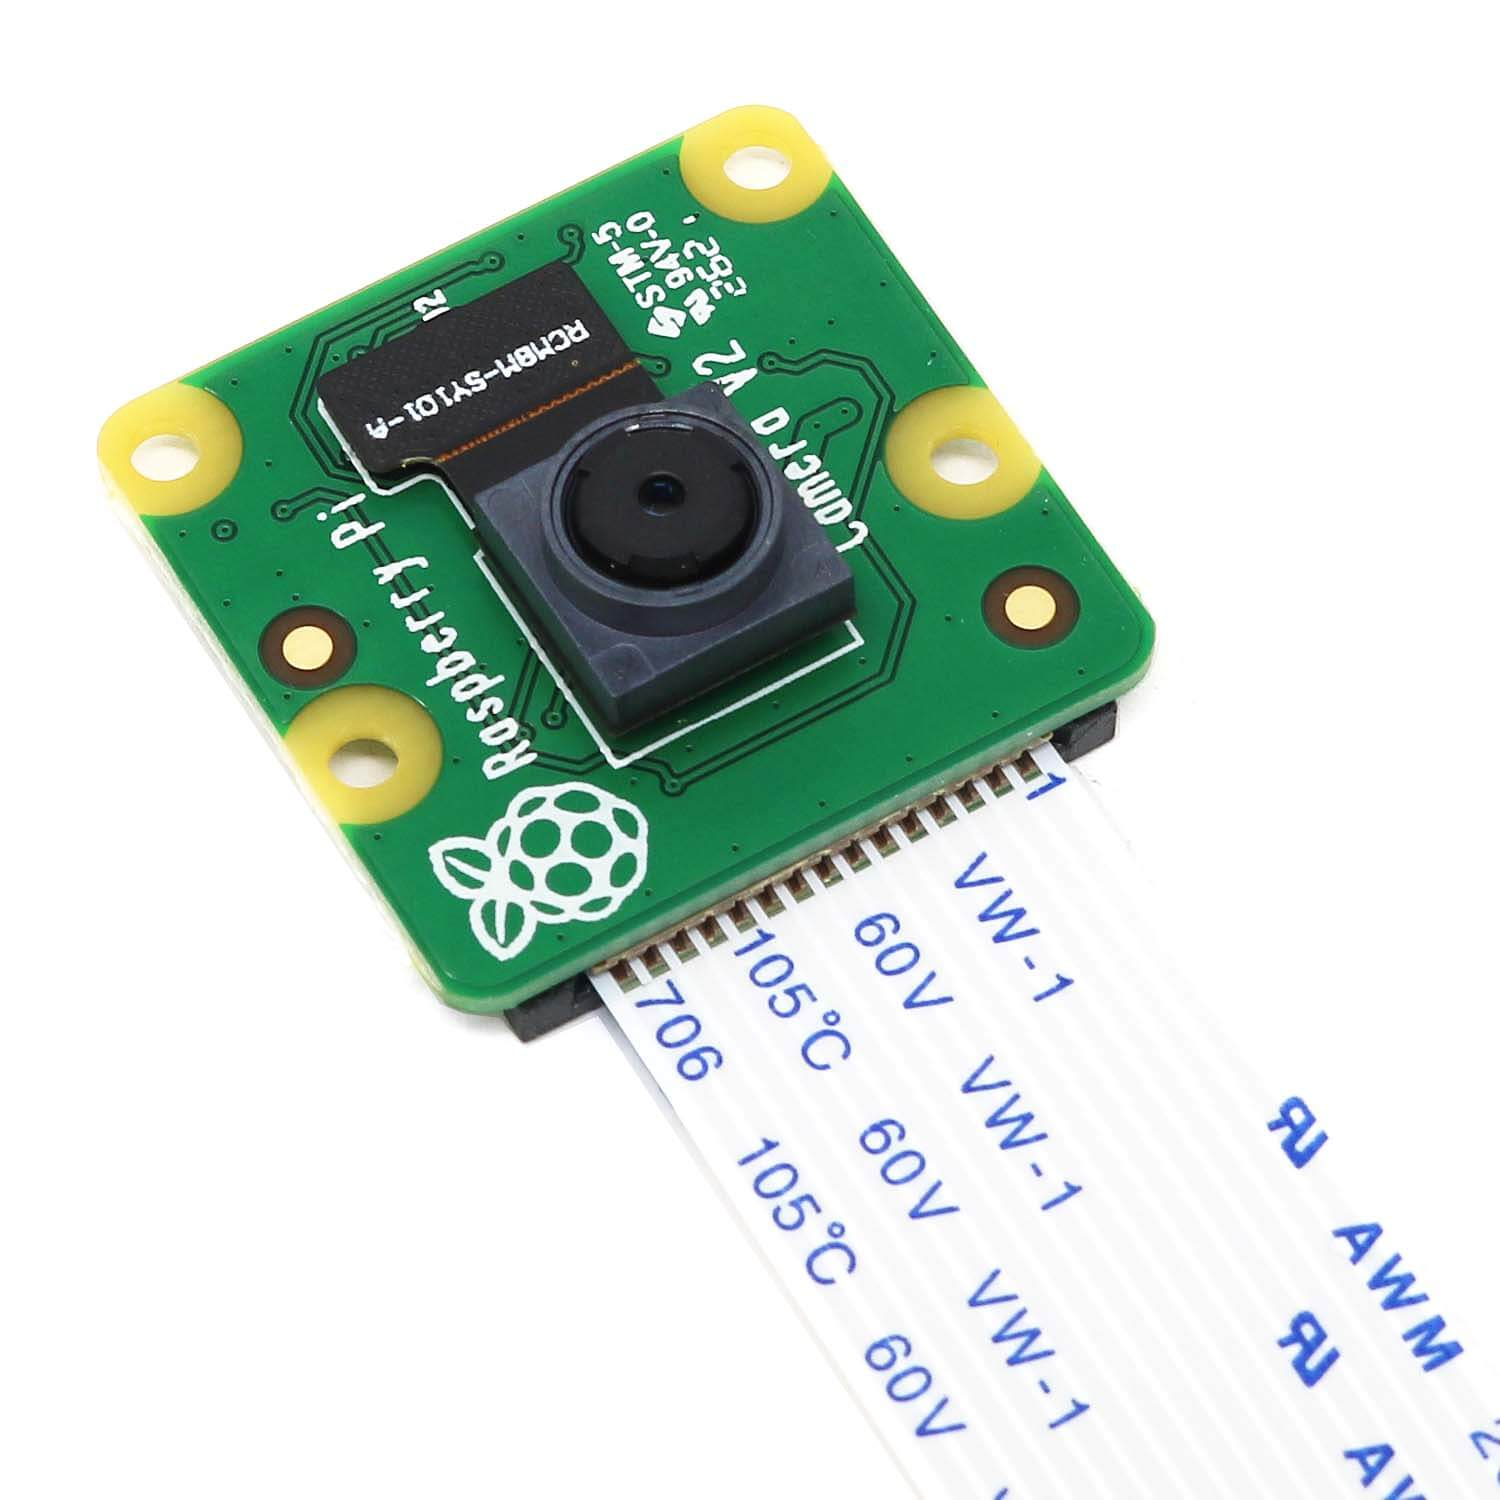
\includegraphics[width=4cm]{figs/picamera}
	\end{center}
	\caption{\textit{PiCamera} usada en la placa \textit{Raspberry Pi}.}
	\label{fig:picamera}
\end{figure}\

Un ejemplo de \textit{FIR} es \textit{BMW's FIR-based Autoliv Night Vision System} \cite{nightvision} (Figura \ref{fig:nightvision}), que trabaja con imágenes de 320 por 240 píxeles y cuenta con un rango de 300 metros. Este sistema utiliza lentes de gran angular que le permiten percibir la imagen con un mayor ángulo de visión.\\

\begin{figure} [h!]
	\begin{center}
		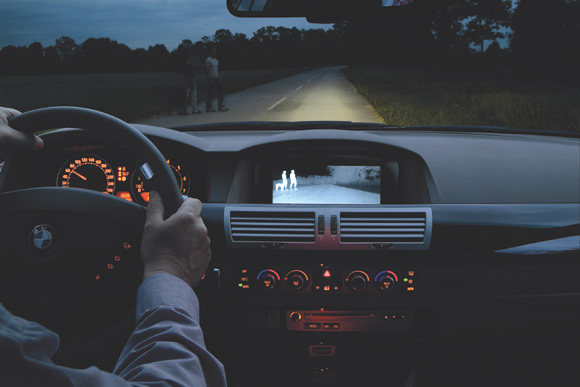
\includegraphics[width=8cm]{figs/nightvision}
	\end{center}
	\caption{Sistema de visión nocturna desarrollado por \textit{BMW}.}
	\label{fig:nightvision}
\end{figure}\

Una información de la imagen que puede resultar de interés es la distancia a la que se encuentra un objeto en concreto. Para calcularla, existen diversas soluciones. Por ejemplo, encontramos una solución con una única cámara, basada en la suposición de que todos los objetos se encuentran situados en el suelo en \cite{vega19d} o \cite{distanceopencv}. Para eliminar esta restricción y poder conocer distancias de objetos que no se encuentran situados en el suelo, surgen las \textit{cámaras RGBD}, en las que cada píxel de la imagen proporciona, además del color \textit{RGB}, una tercera componente, la profundidad o \textit{depth}. Una de las primeras cámaras \textit{RGBD} comerciales es la \textit{Kinect}, desarrollada por \textit{Microsoft} para su consola \textit{Xbox 360} (Figura \ref{fig:kinect}).\\

\begin{figure} [h!]
	\begin{center}
		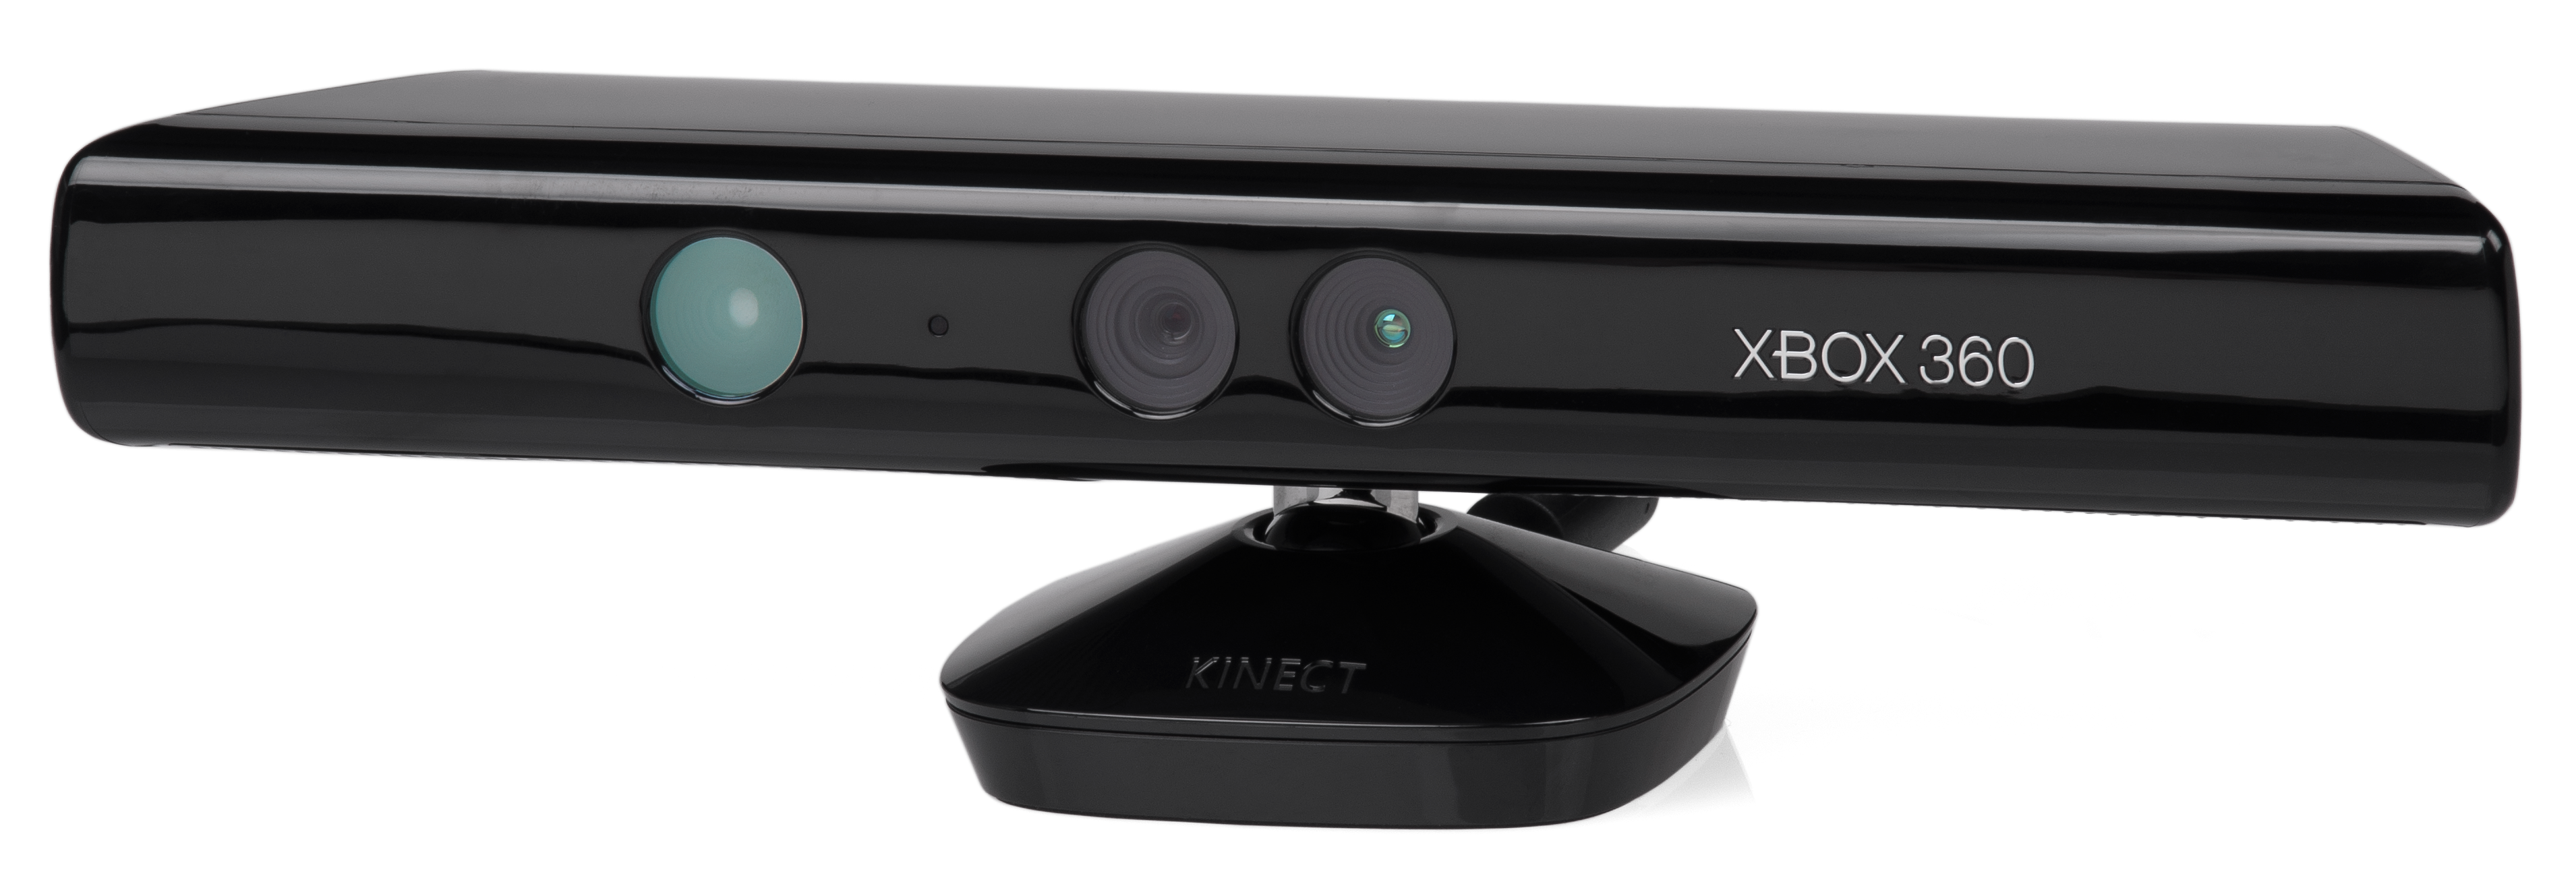
\includegraphics[width=6cm]{figs/kinect}\hspace{0.5cm}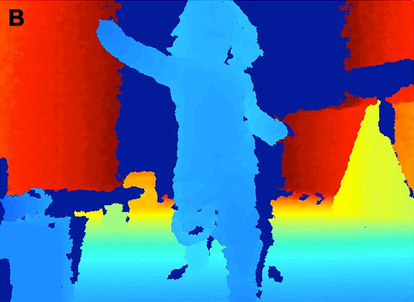
\includegraphics[width=6cm]{figs/depth}
	\end{center}
	\caption{Cámara \textit{RGBD Microsoft Kinect} e imagen de profundidad obtenida por esta.}
	\label{fig:kinect}
\end{figure}\

La visión artificial ofrece multitud de posibilidades, más allá de la robótica, ofrece numerosas aplicaciones en campos tan dispares como la medicina, la realidad aumentada, el procesamiento de señales o la agricultura.\\

\section{Deep Learning}
\label{sec:deeplearning}
El Aprendizaje Profundo, se basa en el uso de redes neuronales artificiales (o {\textit{Artificial Neural Network}}, \textit{ANN}) que parten del aprendizaje automático, \textit{Machine Learning} que a su vez surge de la Inteligencia Artificial. Las redes neuronales están inspiradas en el cerebro humano, donde una neurona se comunica con otra mediante señales. En el caso de su abstracción al mundo de la computación, una red está formada por una capa de entrada, una o más capas internas, y una capa de salida (Figura \ref{fig:neuralnetwork})\footnote{\url{https://www.ibm.com/cloud/learn/neural-networks}}. Estas redes neuronales necesitan ser entrenadas mediante el concepto, anteriormente introducido, de \textit{dataset}. A partir de este entrenamiento, la red es capaz de aprender y aumentar su precisión para que el resultado obtenido tenga fiabilidad.\\

\begin{figure} [h!]
	\begin{center}
		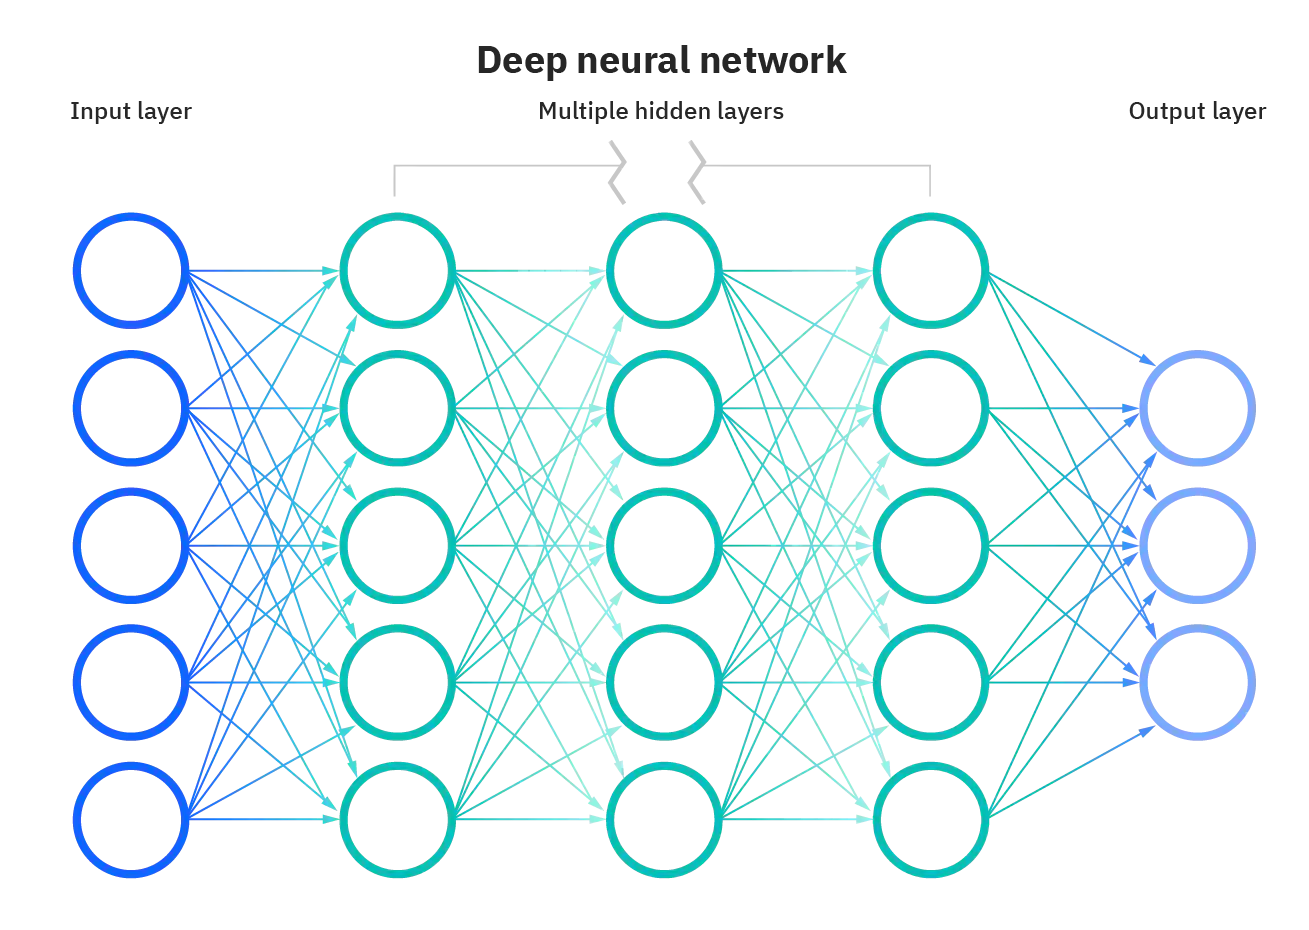
\includegraphics[width=10cm]{figs/neuralnetwork}
	\end{center}
	\caption{Red neuronal con tres capas internas.}
	\label{fig:neuralnetwork}
\end{figure}\

Los inicios del \textit{Deep Learning} se remontan al año 1979, cuando \textit{Kunihiko Fukushima} desarrolló una red neuronal de entre 5 y 6 capas llamada \textit{neocognitrón} \cite{neocognitron}, con el objetivo de reconocer caracteres japoneses.\\

Este tipo de redes neuronales tiene multitud de aplicaciones, pero todas comparten grandes cantidades de datos, en cualquier formato (vídeo, imagen, sonido). Algunas de ellas son: clasificación de objetos, procesamiento natural del lenguaje, \textit{Big Data}, análisis médico, conversión de imágenes en blanco y negro a color etc.\\

\section{Coches autónomos}
\label{sec:cochesautonomos}
Cuando pensamos en un vehículo autónomo, pensamos en un vehículo que circula por la ciudad (coches, autobuses, furgonetas) sin una persona al volante (Figura \ref{fig:volvovera})\footnote{\url{https://www.volvogroup.com/en/news-and-media/news/2019/jun/news-3336083.html}}. Pero, a día de hoy, todavía no está presente en las ciudades aunque cabe esperar que en un corto plazo de tiempo lo esté. El principal inconveniente que actualmente está frenando su implantación es la legislación; a diferencia de, por ejemplo, el entorno de la aviación, donde desde hace décadas el control de la aeronave es automático (a excepción de tareas como el despegue, el aterrizaje o situaciones de emergencia).\\

Actualmente, coches de última generación como \textit{Tesla} (Figura \ref{fig:teslaobjectdetection}), ya incorporan un grado de autonomía elevado en determinadas situaciones, pero siempre con un conductor al volante que debe permanecer atento para poder reaccionar.\\

\begin{figure} [h!]
	\begin{center}
		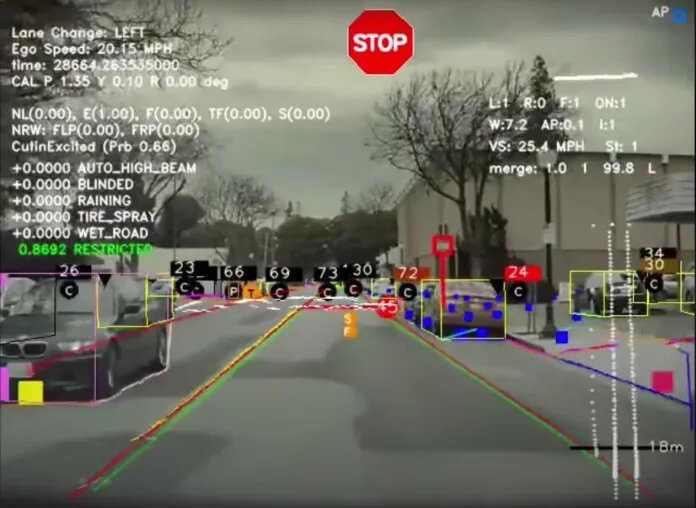
\includegraphics[width=12cm]{figs/teslaobjectdetection}
	\end{center}
	\caption{Sistema de conducción autónoma \textit{Tesla AutoPilot}.}
	\label{fig:teslaobjectdetection}
\end{figure}\

Atendiendo al estándar \textit{SAE J3016} \cite{saej3016} los niveles de autonomía se pueden dividir en cinco:
\begin{enumerate}
	\item Sin automatización: avisos y asistencia puntualmente.
	\item Asistencia a la conducción: centrado de carril o control de crucero.
	\item Automatización parcial: centrado de carril y control de crucero.
	\item Automatización condicionada: conducción automática en atascos.
	\item Automatización elevada: conducción automática en algunas situaciones.
	\item Automatización completa: conducción automática en cualquier situación.
\end{enumerate}\

\begin{figure} [h!]
	\begin{center}
		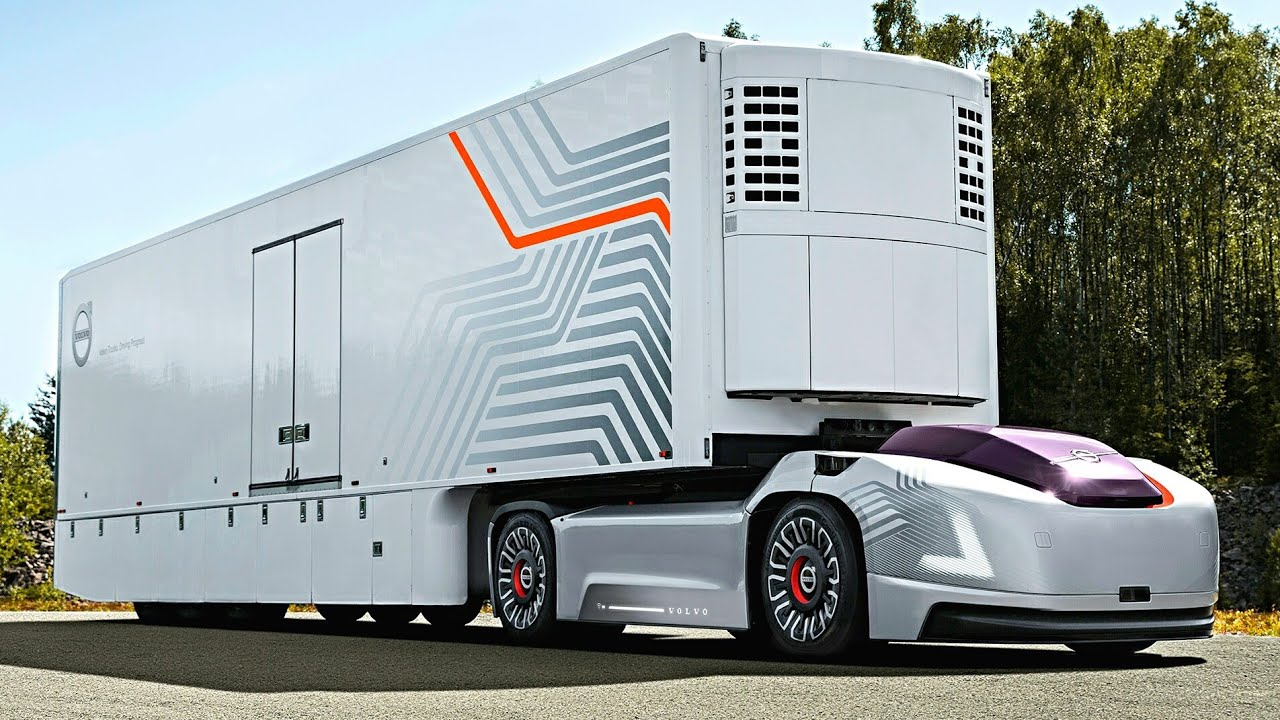
\includegraphics[width=12cm]{figs/volvovera}
	\end{center}
	\caption{Camión autónomo nivel 5 de la marca \textit{Volvo}.}
	\label{fig:volvovera}
\end{figure}\

\subsection{AMRs}
\label{sec:amr}
Los robots móviles autónomos (o \textit{Autonomous Mobile Robot}, \textit{AMR}) son aquellos capaces de navegar por entornos dinámicos, conviviendo con humanos a su alrededor y sabiendo sobreponerse a situaciones para las que no habían sido programados explícitamente. Son los sucesores de los vehículos de guiado automático (o \textit{Automated Guided Vehicle}, \textit{AGV}), los cuales requieren una cierta infraestructura dependiendo del tipo de guiado, ya sea filo-guiados, a través de pintura o a través de cualquier otra técnica que haga que ese vehículo solo pueda funcionar cuando se conoce la infraestructura previa que estará presente en el entorno de trabajo.\\

Por otro lado, estos \textit{AGVs}\footnote{\url{https://mobilerobotguide.com/2021/08/06/whats-the-difference-between-an-amr-and-an-agv/}} presentan muchas dificultades para relacionarse con obstáculos o humanos, donde ante un cambio pequeño del entorno, el robot se detendrá por seguridad. A diferencia de estos, los \textit{AMRs} son capaces de realizar multitud de tareas en entornos donde la infraestructura necesaria es casi nula, quitando alguna necesidad de conectividad. Salvo por esa excepción, son robots que pueden ser diseñados para navegar por cualquier tipo de ambiente.\\

Un ejemplo muy representativo de \textit{AMRs} son los robots de \textit{Kiva Systems}\footnote{\url{https://www.aboutamazon.es/noticias/innovacion/los-robots-en-numeros-datos-y-cifras-sobre-los-robots-en-amazon}} (Figura \ref{fig:kivasystems}), empresa comprada por \textit{Amazon} en 2012\footnote{\url{https://www.eleconomista.es/tecnologia/noticias/3833220/03/12/Amazon-compra-la-empresa-robotica-Kyva-Systems-por-775-millones-de-dolares.html}} para automatizar sus almacenes en tareas de logística a nivel interno, maximizando la productividad y el almacenamiento, tanto en profundidad como en altura, y minimizando el coste en personal.\\

\begin{figure} [h!]
	\begin{center}
		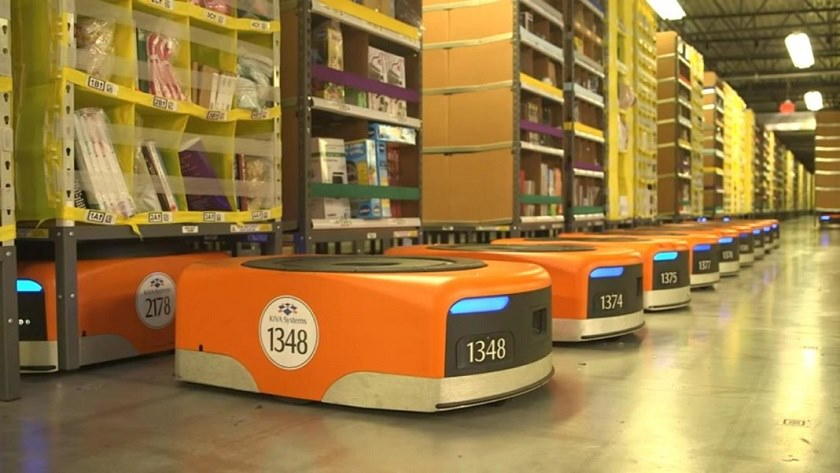
\includegraphics[width=8cm]{figs/kivasystems}
	\end{center}
	\caption{\textit{AMRs} de \textit{Kiva Systems} en almacenes de \textit{Amazon}.}
	\label{fig:kivasystems}
\end{figure}\

El presente trabajo se enmarca dentro del campo de la robótica y la visión artificial. En estas disciplinas se hace uso de todas estas tecnologías con el objetivo de dotar a los robots de una cierta inteligencia. En los próximos capítulos se detallarán los objetivos a cumplir, las plataformas utilizadas y el diseño implementado.

\chapter{Objetivos}
\label{cap:capitulo2}

En este capítulo se detallan los objetivos del trabajo realizado, así como, los requisitos que este ha de cumplir, la metodología utilizada y el plan de trabajo seguido para completarlo.\\

\section{Descripción del problema}
\label{sec:descripcion}

El objetivo del trabajo es implementar un coche autónomo bajo una plataforma de bajo coste y reducido tamaño capaz de circular por un circuito o carretera en un entorno dinámico interactuando con objetos propios de una ciudad, como semáforos, señales de stop o peatones. Para ello se ha dividido el objetivo en general en dos subobjetivos:

\begin{enumerate}[(a)]
	\item Entorno simulado: utilizando el entorno de simulación \textit{Gazebo} se desarrollará el problema anteriormente descrito con la finalidad de, posteriormente, realizar lo mismo en un entorno real.\\
	\item Entorno real: utilizando un robot real diseñado a partir de la placa \textit{NVIDIA Jetson Nano}, se desarrollará el problema anteriormente descrito sobre un circuito construido a partir de pistas de \textit{Scalextric}\footnote{\url{https://scalextric.es/}}.\\
\end{enumerate}\

Como se dijo anteriormente, en ambos entornos, se ha de completar dos objetivos:

\begin{enumerate}[(a)]
	\item Seguimiento de carril: el coche autónomo tendrá que ser capaz de realizar un seguimiento del carril utilizando una red neuronal que indicará el centro del carril al que el robot deberá ceñirse.
	\item Detección de objetos: mientras el robot realiza el seguimiento del carril debe interactuar con objetos del entorno, esto es, reaccionar cuando ve una señal de stop o un semáforo y rojo y detenerse apropiadamente. Está detección deberá ser realizada, preferiblemente, en tiempo real.
\end{enumerate}\

\section{Requisitos}
\label{sec:requisitos}
El trabajo tendrá una serie de requisitos que deberán ser respetados:
\begin{enumerate}
	\item El sistema operativo utilizado, para ambos entornos, será \textit{GNU/Linux}, concretamente la distribución \textit{Ubuntu} 20.04 LTS ya que cuenta con soporte para múltiples arquitecturas y proporciona un gran rendimiento.
	\item El entorno simulado requerirá la presencia de una tarjeta gráfica dedicada ya que es muy recomendable para trabajar con redes neuronales; concretamente de la marca \textit{NVIDIA}, ya que se utilizará la plataforma \textit{CUDA}.
	\item El entorno real requerirá un robot con la placa de desarrollo \textit{NVIDIA Jetson Nano} debido a ser una de las placas con \textit{GPU} más económicas.
	\item El lenguaje de programación utilizado será \textit{Python} debido a las librerías utilizadas, que se detallarán en el próximo capítulo.
\end{enumerate}\

\section{Metodología}
\label{sec:metodologia}
Partiendo de los requisitos y objetivos previamente descritos, se procedió a evaluar el hardware necesario; a continuación, se realizó un análisis de diversas bibliotecas de código con el objetivo de seleccionar las que fuesen compatibles y tuviesen un mejor rendimiento en la plataforma de hardware elegida. El siguiente paso fue el diseño del software necesario y cómo integrarlo con las bibliotecas escogidas. Por último se realizaron pruebas periódicas tanto en simulador como en un entorno real, con el objetivo de ir afinando el software para conseguir el resultado final.\\

\section{Plan de trabajo}
\label{sec:plantrabajo}

El plan de trabajo se ha basado en reuniones semanales o quincenales con el tutor, dependiendo de la carga de trabajo, en las que se iban fijando objetivos específicos y fijando la estrategia para poder completar el proyecto.\\

Todo el trabajo realizado se ha ido subiendo a un repositorio de trabajo en \textit{GitHub}\footnote{\url{https://github.com/jmvega/tfg-amariscal}}. De esta forma se podía analizar de forma muy rápida los cambios realizados en el código. También se ha ido desarrollando una \textit{Wiki}\footnote{\url{https://github.com/jmvega/tfg-amariscal/wiki}} en \textit{GitHub} a modo de bitácora en la que se iban detallando los avances del proyecto, así como, los problemas y las limitaciones que iban surgiendo a medida que se cumplían los objetivos.\\


\chapter{Plataforma de desarrollo}
\label{cap:capitulo3}

\begin{flushright}
	\begin{minipage}[]{10cm}
		\emph{Quizás algún fragmento de libro inspirador...}\\
	\end{minipage}\\

	Autor, \textit{Título}\\
\end{flushright}

\vspace{1cm}

En este capítulo, se explica el hardware y software elegido para desarrollar el trabajo y los motivos de dicha elección.

\section{Hardware}
\subsection{\textit{NVIDIA Jetson Nano}}
\label{subsection:jetsonnanoo}
La placa de desarrollo \textit{NVIDIA Jetson Nano}\footnote{\url{https://developer.nvidia.com/embedded/jetson-nano}} es una plataforma de bajo coste con grandes capacidades computacionales para implementar técnicas de inteligencia artificial gracias a su \textit{GPU} dedicada \textit{NVIDIA Maxwell}\footnote{\url{https://developer.nvidia.com/maxwell-compute-architecture}} con 128 \textit{NVIDIA CUDA cores}\footnote{\url{https://developer.nvidia.com/cuda-gpus}}, además dispone de una CPU Quad-core basada en la arquitectura Aarch64 lo que permite ejecutar GNU/Linux sin dificultades y ser compatible con numerosas bibliotecas de código. La placa en cuestión, dispone además de pines GPIO lo que permite de forma muy sencilla conectar todo tipo de sensores y actuadores.\\

Los requisitos en lo que a alimentación se refiere no son excesivos, requiere un mínimo de 5 voltios (V) y 3 amperios (A), lo que permite que una simple \textit{powerbank} de reducido tamaño sea capaz de alimentar la placa, si bien es cierto que la batería debe poder ofrecer tres amperios de forma estable, y no solo como intensidad pico. Existen numerosos proyectos en los que esta placa está presente, tales como JetBot\footnote{\url{https://github.com/NVIDIA-AI-IOT/jetbot}} o JetRacer\ref{subsection:jetracer}.\\

\begin{figure} [h!]
	\begin{center}
		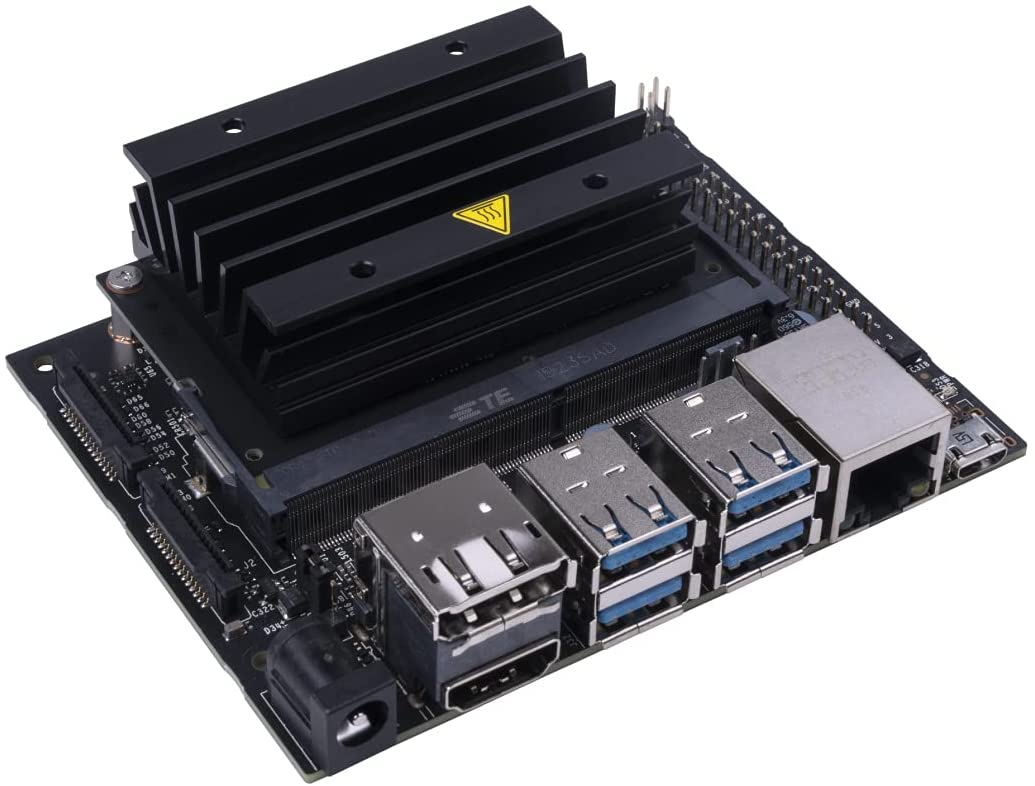
\includegraphics[width=4cm]{figs/jetsonnano}
	\end{center}
	\caption{\textit{NVIDIA Jetson Nano}.}
	\label{fig:jetsonnano}
\end{figure}\

\subsection{Motores \textit{TT}}
\label{subsection:motortt}
Se trata de unos motores\footnote{\url{https://www.verical.com/datasheet/adafruit-brushless-dc-motors-3777-5912007.pdf}} de corriente continua con reductora utilizados en la multitud de proyectos de robótica de muy bajo coste\footnote{\url{https://github.com/grimmpp/tt-motor-mounting}}\footnote{\url{https://github.com/bhabegger/diy-telepresence-robot}}. La tensión de alimentación tiene un rango de 3 a 6 voltios y la velocidad mínima en vacío tiene un rango de 90 a 200 revoluciones por minuto (RPM) dependiendo del voltaje, lo que permite conseguir una velocidad reducida para robots de pequeño tamaño.\\

\begin{figure} [h!]
	\begin{center}
		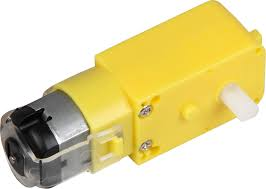
\includegraphics[width=4cm]{figs/motorTT}
	\end{center}
	\caption{Motores \textit{TT}.}
	\label{fig:motorTT}
\end{figure}\

\subsection{Controladora de motores \textit{L298N}}
\label{subsection:l298no}
Es un módulo\footnote{\url{https://www.luisllamas.es/arduino-motor-corriente-continua-l298n/}} capaz de controlar la dirección y la velocidad de los motores anteriormente citados. La tensión de alimentación es de un mínimo de 6 voltios, lo que hace imposible alimentarla con la placa \textit{NVIDIA Jetson Nano}\ref{fig:jetsonnano} por lo que es necesario una batería externa. Otra posibilidad para utilizar una única batería sería utilizar la salida de 5 voltios (V) que nos ofrece la controladora, sin embargo, dicha salida nunca ofrecerá los 3 amperios (A) requeridos. Este componente permite invertir el sentido de la corriente lo que proporciona un control para mover los motores en el sentido de las agujas del reloj (CW) y en el sentido contrario a las agujas del reloj (CCW). La principal limitación de esta placa es que solo permite controlar dos motores, por lo que si se dispone de 4 motores, se podrán conectar a pares dependiendo del comportamiento deseado. El control se realiza a través de la técnica PWM\footnote{\url{https://circuitdigest.com/tutorial/what-is-pwm-pulse-width-modulation}}, que permite enviar de forma precisa la velocidad deseada a través de una señal digital.\\

\begin{figure} [h!]
	\begin{center}
		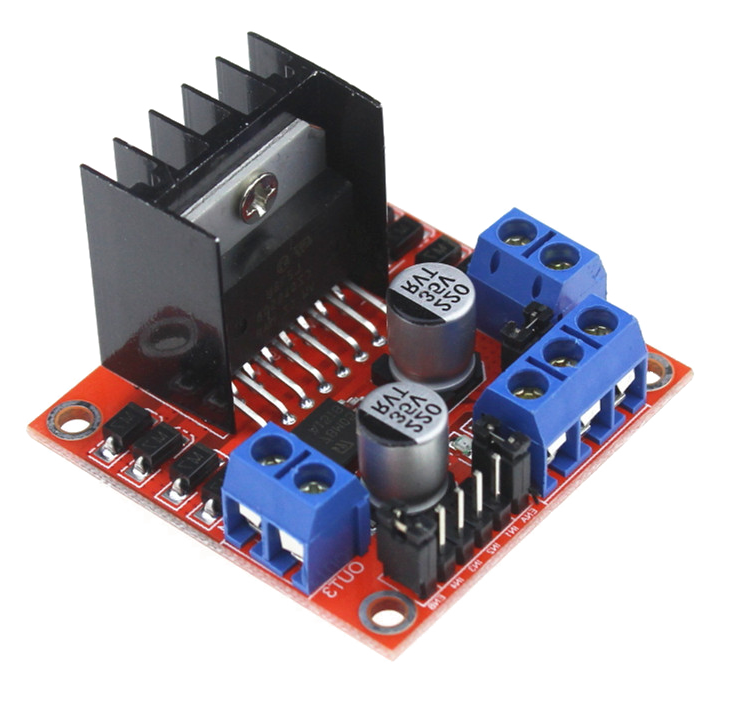
\includegraphics[width=4cm]{figs/l298n}
	\end{center}
	\caption{Controladora de motores \textit{L298N}.}
	\label{fig:l298n}
\end{figure}\

\subsection{Cámara \textit{Xiaomi}}
\label{subsection:xiaomicamerao}
Se trata de una cámara USB\ref{fig:xiaomicamera} lo que permite recibir la imagen a través de dicho puerto con una tasa de 30 \textit{frames} por segundo (FPS). Su resolución es 1080p\footnote{\url{https://xiaomiplanets.com/xiaovv-6320s-webcam-5/}} pero permite obtener una imagen de menor resolución a través de su driver.\\

\begin{figure} [h!]
	\begin{center}
		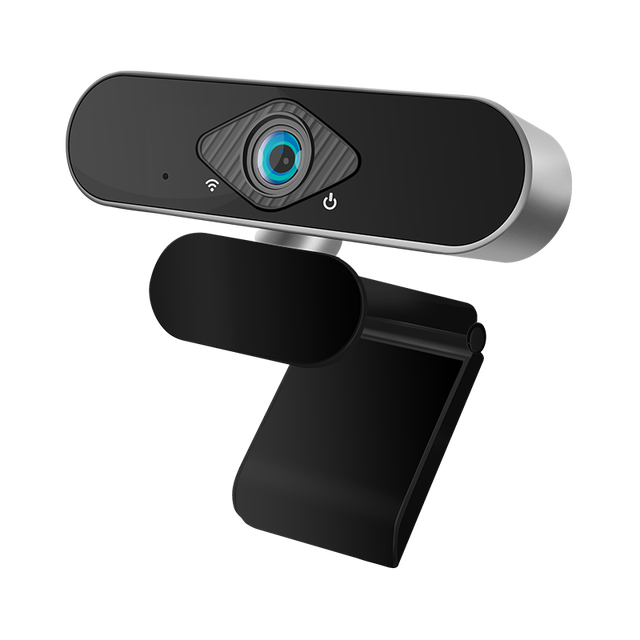
\includegraphics[width=4cm]{figs/camera}
	\end{center}
	\caption{Cámara \textit{Xiaomi}.}
	\label{fig:xiaomicamera}
\end{figure}\

\subsection{Batería 10000mAh}
\label{subsection:batteryo}
Su capacidad es de 10000 miliamperios hora (mAh), el voltaje de funcionamiento es 5 voltios (V) y su intensidad teórica es 3 amperios (A) por lo que permite alimentar la placa \textit{NVIDIA Jetson Nano}\ref{fig:jetsonnano}.\\

\begin{figure} [h!]
	\begin{center}
		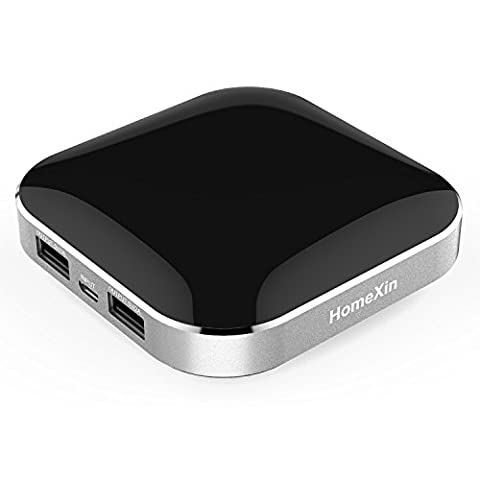
\includegraphics[width=4cm]{figs/battery}
	\end{center}
	\caption{Batería 10000mAh.}
	\label{fig:battery}
\end{figure}\

\subsection{Chasis}
\label{subsection:chasio}
Se trata de un chasis\ref{fig:chasis} de bajo coste muy común en proyectos relacionados con Arduino. Dispone de soportes para los Motores \textit{TT}\ref{fig:motorTT}, lo que perimite ensamblarlos de forma muy sencilla. El tamaño es suficiente para alojar todos los componentes elegidos utilizando los agujeros predefinidos en el chasis.\\

\begin{figure} [h!]
	\begin{center}
		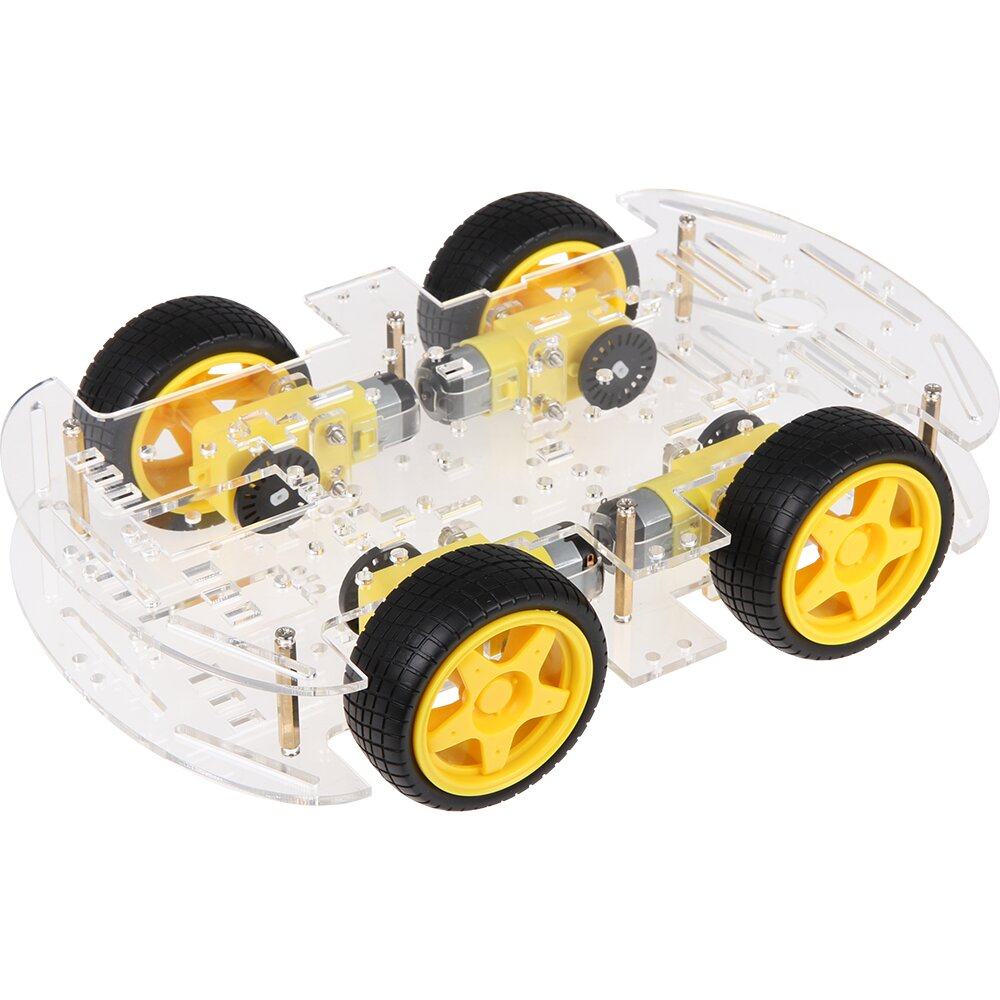
\includegraphics[width=4cm]{figs/chasis}
	\end{center}
	\caption{Chasis.}
	\label{fig:chasis}
\end{figure}\

\section{Software}

\subsection{\textit{Python}}
\label{subsection:pythono}
\textit{Python} es un lenguaje de programación de código abierto, interpretado, orientado a objetos y de alto nivel. En la actualidad es el lenguaje más usado a nivel mundial\footnote{\url{https://pypl.github.io/PYPL.html}}. Está considerado como un lenguaje fácil de aprender gracias a su simple sintáxis, esto le ha llevado a crecer mucho en popularidad durante los últimos años. Además, al ser interpretado, no es necesario utilizar un compilador, lo que provoca un desarrollo mucho más rápido. Python cuenta con una enorme cantidad de bibliotecas y clientes para utilizar software desarrollado en otros lenguajes. Algunas de ellas se describirán a continuación.\\

\subsection{\textit{Blender}}
\label{subsection:blendero}
\textit{Blender}\footnote{\url{https://www.blender.org/}} es una plataforma de código abierto dedicada a la creación, simulación, renderizado y animación de modelos 3D con todo tipo de texturas, sombras etc.. Es un desarrollo de la Blender Foundation y está escrito principalmente en \textit{C}. Permite crear diseños de robots desde cero de una forma relativamente rápida.\\

\begin{figure} [h!]
	\begin{center}
		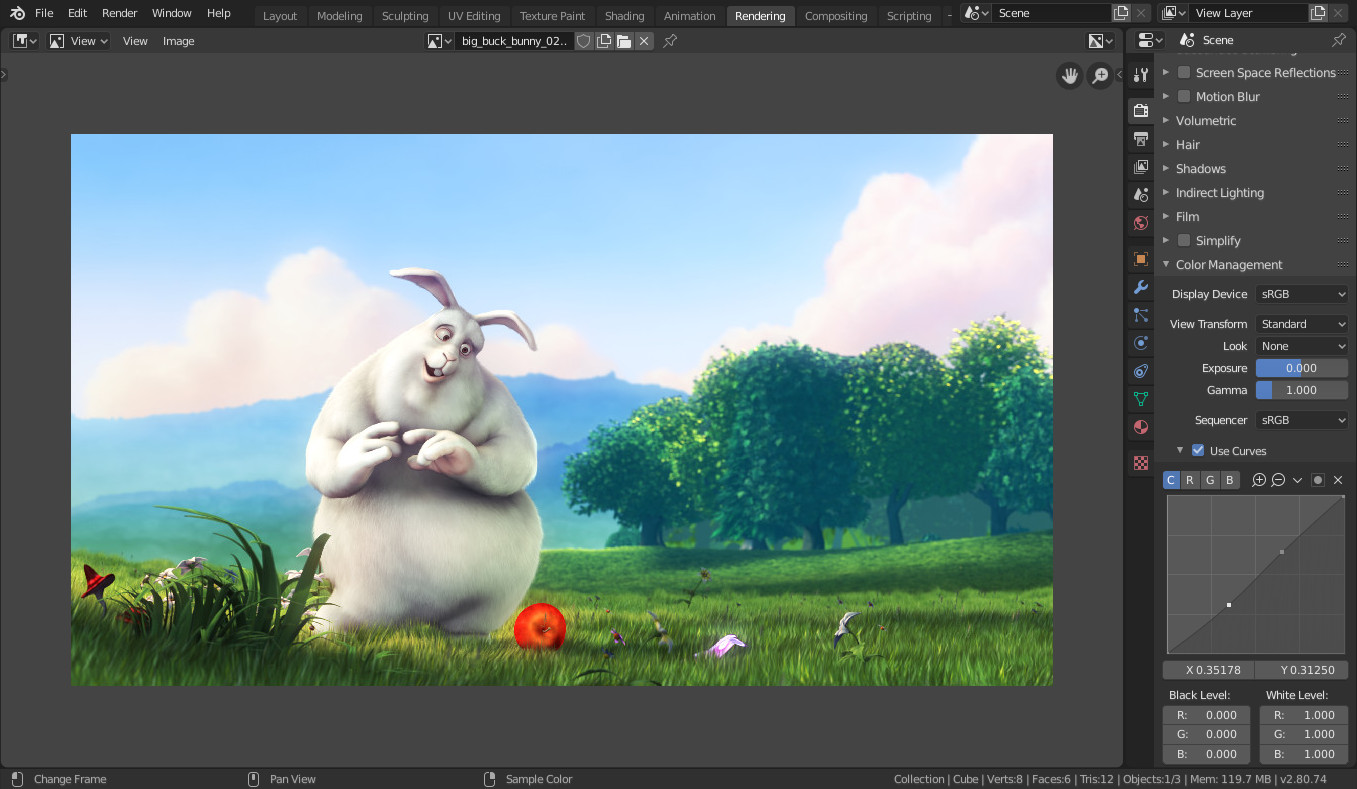
\includegraphics[width=10cm, height=6cm]{figs/blender}
	\end{center}
	\caption{Creación de una animación 3D con \textit{Blender}.}
	\label{fig:blender}
\end{figure}\

\subsection{\textit{Gazebo}}
\label{subsection:gazeboo}
\textit{Ignition Gazebo}\footnote{\url{https://github.com/gazebosim/gz-sim}} es un simulador 3D de código abierto desarrollado por la \textit{Open Source Robotics Foundation (OSRF)}\footnote{\url{https://www.openrobotics.org/}}, escrito en \textit{C++}, usado principalmente para simular comportamientos con gran precisión y gráficos de alta calidad en los que intervienen robots en un entorno dinámico\ref{fig:city}. Desde  Utiliza, por defecto, el motor de físicas \textit{ODE}\footnote{\url{https://bitbucket.org/odedevs/ode/src/master/}}, escrito también en \textit{C++}. Permite simular todo tipo de sensores y actuadores. Además, ofrece integración con ROS de forma muy sencilla.\\

\begin{figure} [h!]
	\begin{center}
		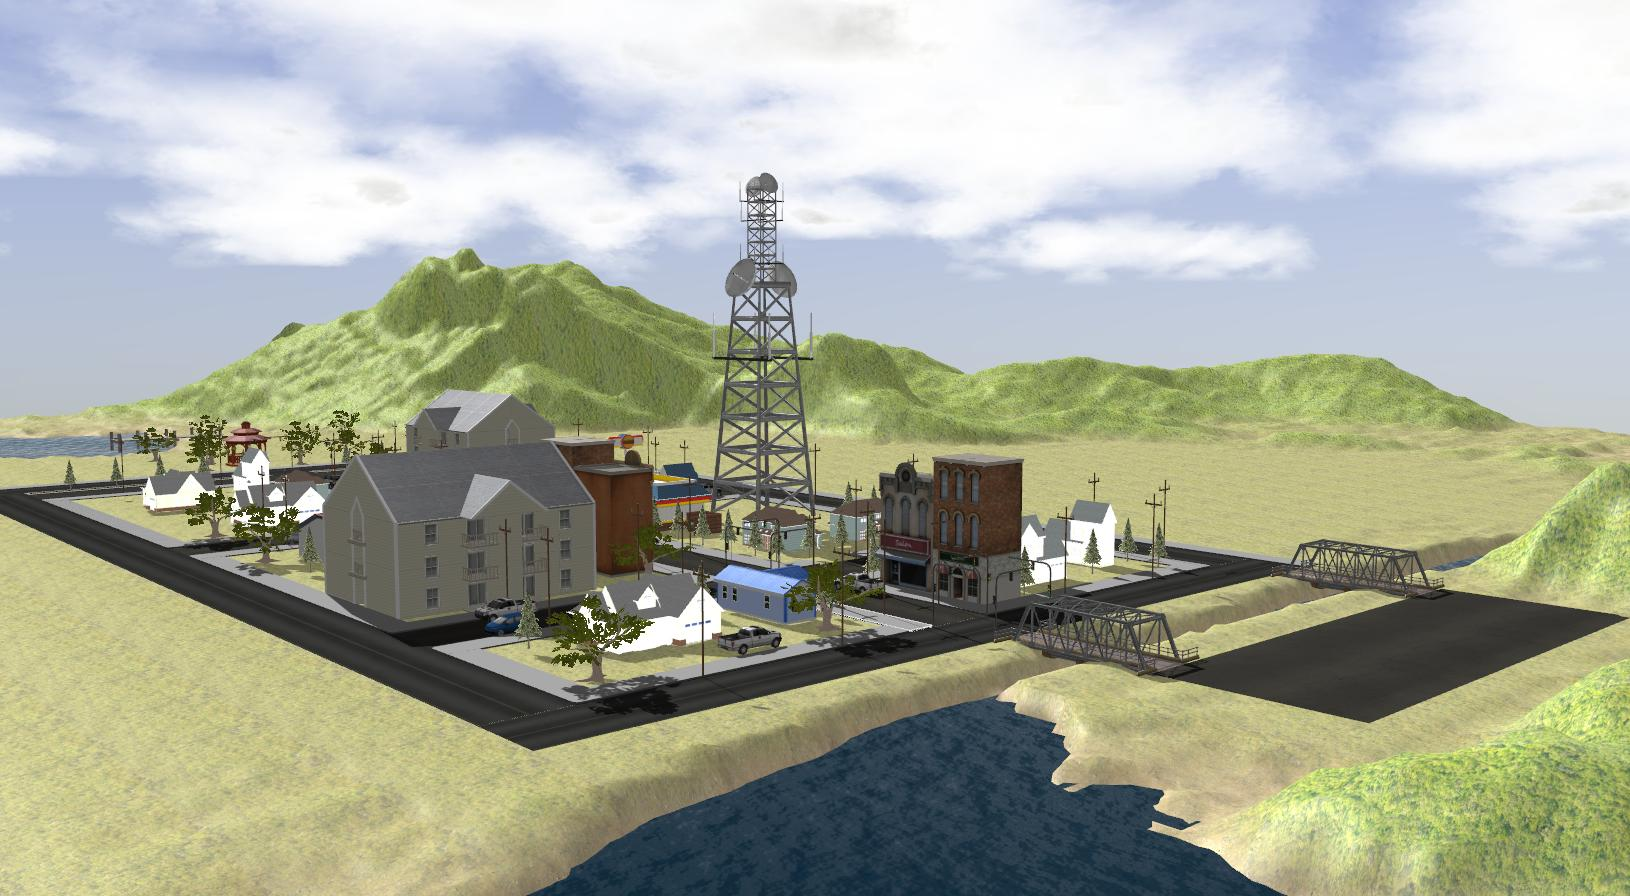
\includegraphics[width=10cm]{figs/city}
	\end{center}
	\caption{Ciudad simulada en \textit{Gazebo}.}
	\label{fig:city}
\end{figure}\

\subsection{\textit{SDF}}
\label{subsection:sdf}
El formato \textit{SDF} (\textit{Simulation Description Format})\footnote{\url{https://github.com/gazebosim/sdformat}} o \textit{SDFormat} permite describir entornos, objetos dinámicos o robots de una manera sencilla. Está basado en \textit{XML} y escrito en \textit{C++}. El objetivo de este formato es ejecutar comportamientos en un simulador. Originalmente fue desarrollado como parte de \textit{Gazebo} por lo que existen numerosas bibliotecas donde se encuentran modelos o mundos desarrollados en \textit{SDF} para este simulador\footnote{\url{https://github.com/HuyPhamG/simulatedswarm}}. Cabe destacar también, el formato URDF que, a diferencia de \textit{SDF}, únicamente puede describir un objeto o robot, pero no el mundo en el que vive\footnote{\url{https://newscrewdriver.com/2018/07/31/ros-notes-urdf-vs-gazebo-sdf/}}.\\

\begin{figure} [h!]
	\begin{center}
		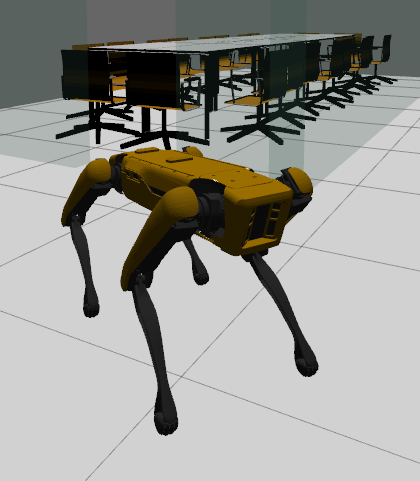
\includegraphics[width=6cm]{figs/spot}
	\end{center}
	\caption{Robot Spot de Boston Dynamics simulado en \textit{Gazebo}.}\footnote{\url{https://github.com/osrf/subt}}
	\label{fig:spot}
\end{figure}\

\subsection{\textit{ROS}}
\label{subsection:ros}
\textit{Robot Operating System ROS}\footnote{\url{https://ros.org/}} es un middleware róbotico, de código abierto, con multitud de bibliotecas y herramientas desarrollado por la \textit{Open Source Robotics Foundation (OSRF)}\footnote{\url{https://www.openrobotics.org/}}, escrito en \textit{C++} y \textit{Python}. Es considerado actualmente el estándar en robótica. Permite desarrollar aplicaciones complejas en las intervienen diversos procesos llamados nodos\footnote{\url{http://wiki.ros.org/Nodes}}, que se comunican entre ellos mediante \textit{topics}\footnote{\url{http://wiki.ros.org/Topics}} y servicios\footnote{\url{http://wiki.ros.org/Services}}. Una de las principales ventajas de utilizar un middleware como ROS es la capacidad de abstracción que proporciona, de forma que el usuario únicamente programa sobre una interfaz\footnote{\url{http://wiki.ros.org/Client20Libraries}} dada, disponible en \textit{C++} y \textit{Python}, sin preocuparse por lo que pasa por debajo.\\

\subsection{\textit{OpenCV}}
\label{subsection:opencv}
\textit{OpenCV}\footnote{\url{https://github.com/opencv/opencv}} es una librería de visión artificial de código abierto desarrollado por Intel\footnote{\url{https://opencv.org/opencv-platinum-membership/}}. Está escrita en \textit{C/C++} y cuenta con soporte para aceleración por GPU basadas en CUDA\footnote{\url{https://developer.nvidia.com/cuda-zone}} y OpenCL\footnote{\url{https://www.khronos.org/opencl/}} y procesamiento de imagen en tiempo real. Es usada en todo tipo de aplicaciones en las que interviene la visión por ordenador, tales como, detección de objetos, realidad aumentada o reconocimiento de gestos. Además, está disponible en multitud de lenguajes de programación; \textit{C++}, \textit{Python}, \textit{Java}, etc...\\

\subsection{\textit{Darknet}}
\label{subsection:darknet}
\textit{Darknet}\footnote{\url{https://pjreddie.com/darknet/}} es un framework de código abierto que permite ejecutar y entrenar redes neuronales en tiempo real, ya que soporta tanto computación por CPU como GPU. Está escrito en C y CUDA, gracias a estar escrito en un lenguaje considerado de bajo nivel, ofrece un rendimiento aceptable en plataformas de bajo coste como \textit{NVIDIA Jetson Nano}\ref{fig:jetsonnano}.\\

\subsection{\textit{PyQt}}
\label{subsection:pyqt}
\textit{PyQt}\footnote{\url{https://pythonpyqt.com/what-is-pyqt/}} es una plataforma de código abierto que permite crear interfaces gráficas (\textit{GUI}) con el framework \textit{Qt} utilizando \textit{Python}, lo que simplifica mucho el desarrollo. Existen multitud de aplicaciones, desde un navegador\footnote{\url{https://github.com/qutebrowser/qutebrowser}} controlado únicamente con el teclado al estilo \textit{VIM}\footnote{\url{https://github.com/vim/vim}}, hasta un software de impresión 3D como \textit{Cura}\ref{fig:cura}.\\

\begin{figure} [h!]
	\begin{center}
		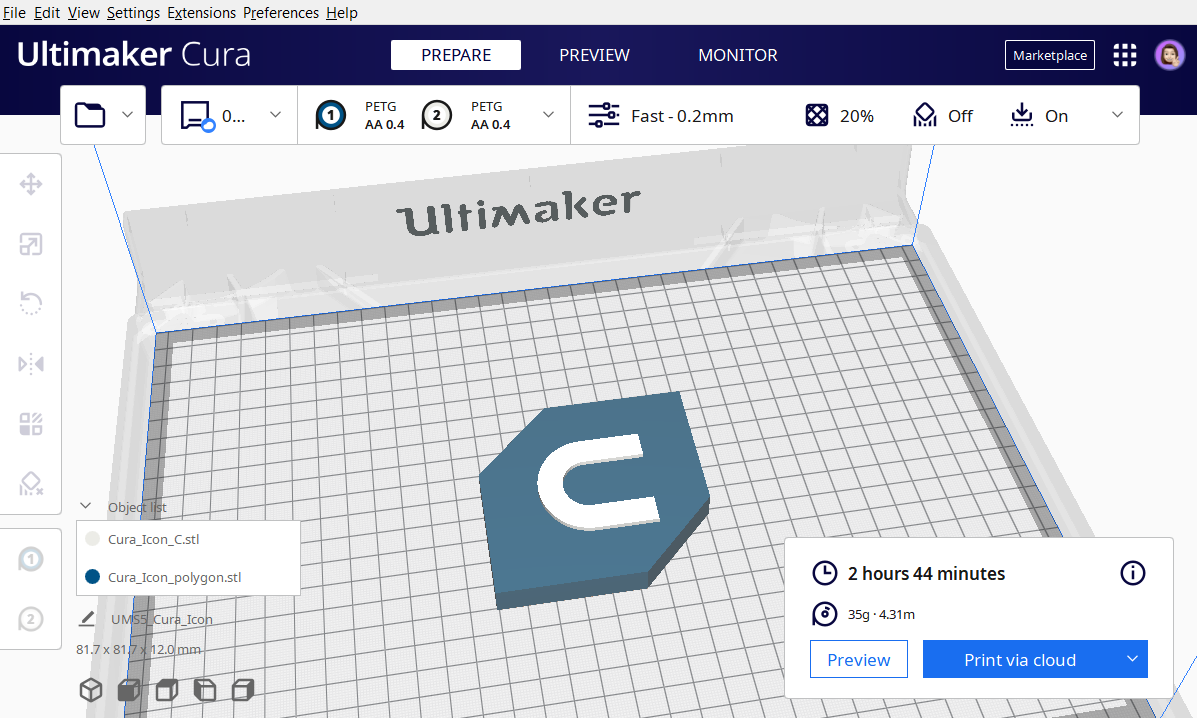
\includegraphics[width=10cm]{figs/cura}
	\end{center}
	\caption{Software de impresión 3D \textit{Ultimaker Cura}.}
	\label{fig:cura}
\end{figure}\

\subsection{\textit{JetRacer}}
\label{subsection:jetracer}
La biblioteca \textit{JetRacer}\footnote{\url{https://github.com/NVIDIA-AI-IOT/jetracer}} permite entrenar una red neuronal para seguir un circuito o una ruta determinada. Utiliza \textit{notebooks} de \textit{Jupyter} para poder reducir la complejidad en el entrenamiento de la red y en el ajuste del controlador\ref{fig:livejetracer}.\\

A su vez esta librería utiliza otras tres cruciales para poder implementar su software:

\begin{itemize}
	\item PyTorch\footnote{\url{https://github.com/pytorch/pytorch}}: es una librería de código abierto con multitud de herramientas para implementar algoritmos de \textit{Deep Learning} basada en \textit{Python}\cite{autopilottesla}. Es un desarrollo de \textit{Facebook's AI Research Lab}. Soporta aceleración por GPU, lo que es esencial para poder ejecutar redes neuronales. Junto a \textit{Tensorflow} y \textit{Keras}, son los tres \textit{frameworks} de referencia en lo que a \textit{Deep Learning} se refiere.
	\item PyTorch to TensorRT\footnote{\url{https://github.com/NVIDIA-AI-IOT/torch2trt}}: permite convertir modelos de PyTorch a modelos optimizados aprovechando los tensores de las gráficas dedicadas y realizando inferencia utilizando operaciones con \textit{FP16} y \textit{FP32}.
	\item Torchvision\footnote{\url{https://github.com/pytorch/vision}}: contiene multitud de \textit{datasets}, modelos preentrenados y algoritmos relacionados con el procesamiento de imagen.
\end{itemize}\

\begin{figure} [h!]
	\begin{center}
		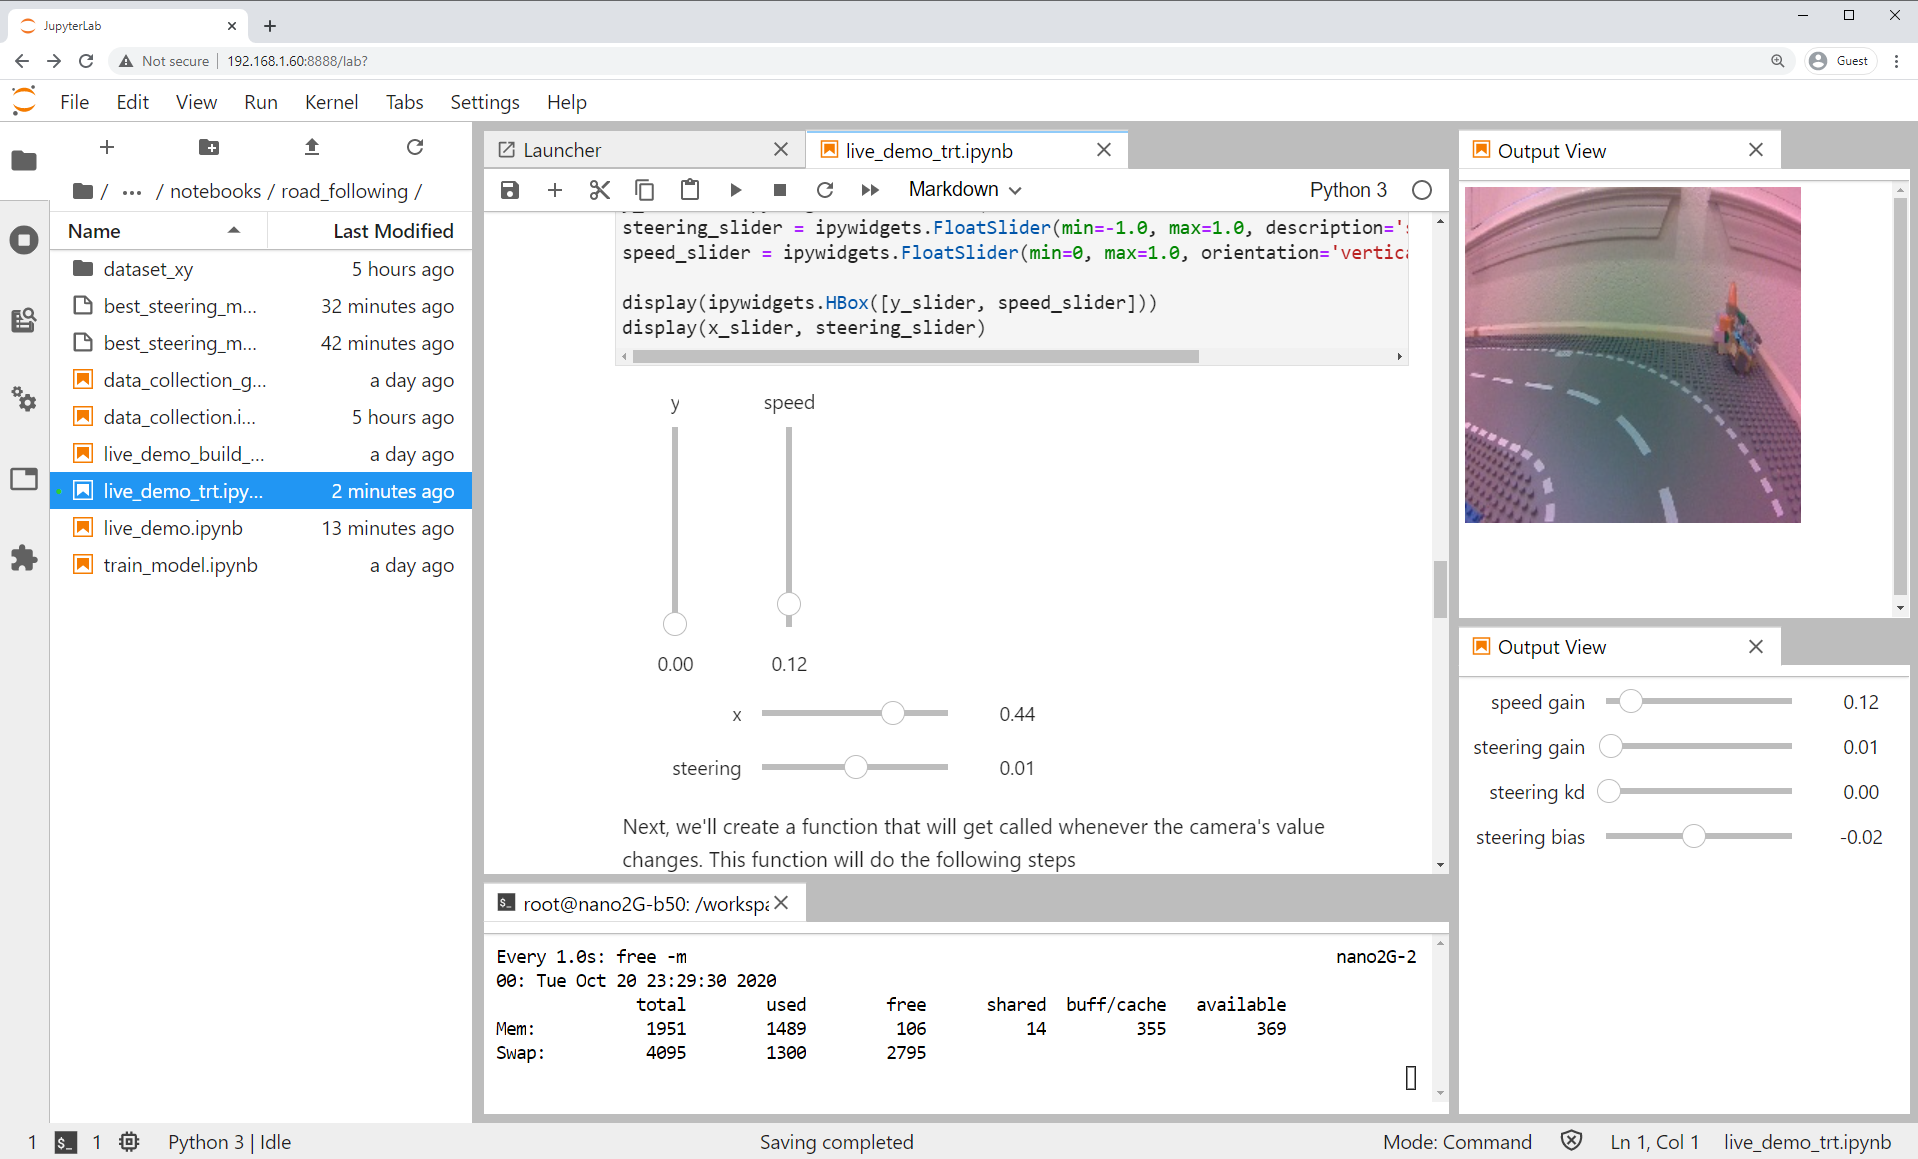
\includegraphics[width=3cm]{figs/livejetracer}
	\end{center}
	\caption{Interfaz \textit{notebook} para ajustar controlador P.}
	\label{fig:livejetracer}
\end{figure}\

Mapa\\
http://wiki.ros.org/Client%20Libraries
\\Referencias del capítulo 2 al 3?\\
h! h!! t!, t!!, T! no compila

\chapter{Diseño}
\label{cap:capitulo4}

En este capítulo se describe el trabajo realizado y los experimentos llevados a cabo para validar el desarrollo.\\

El trabajo, como se explicó en el Capítulo 2, se ha dividido en dos fases; primero se realiza una simulación del coche autónomo en una ciudad simplificada, para a continuación, reproducir ese mismo escenario en un entorno real.\\

\section{Entorno simulado}
\label{section:simulation}
Para poder simular el comportamiento deseado en un entorno simulado es necesario disponer de dos elementos; un modelo del coche autónomo y un mundo dinámico con el que el vehículo interactuará, todo ello ejecutado dentro de un simulador, en este caso, como se explicó anteriormente, en \textit{Gazebo}.\\

\subsection{Modelo de la ciudad}
\label{subsection:citymodel}
Existen numerosos mundos diseñados para \textit{Gazebo} disponibles en repositorios de \textit{GitHub}\footnote{\url{https://github.com/chaolmu/gazebo_models_worlds_collection}}\footnote{\url{https://github.com/mlherd/Dataset-of-Gazebo-Worlds-Models-and-Maps}}. En el caso que se plantea, es necesario una ciudad, por lo que partiendo de una ciudad\footnote{\url{https://github.com/chaolmu/gazebo_models_worlds_collection/blob/master/worlds/small_city.world}} de gran tamaño se reduce su tamaño con el objetivo de, posteriormente, poder reproducir ese escenario en el mundo real. En la Figura \ref{fig:cityversus} se observan ambas ciudades.\\

\begin{figure} [h!]
	\begin{center}
		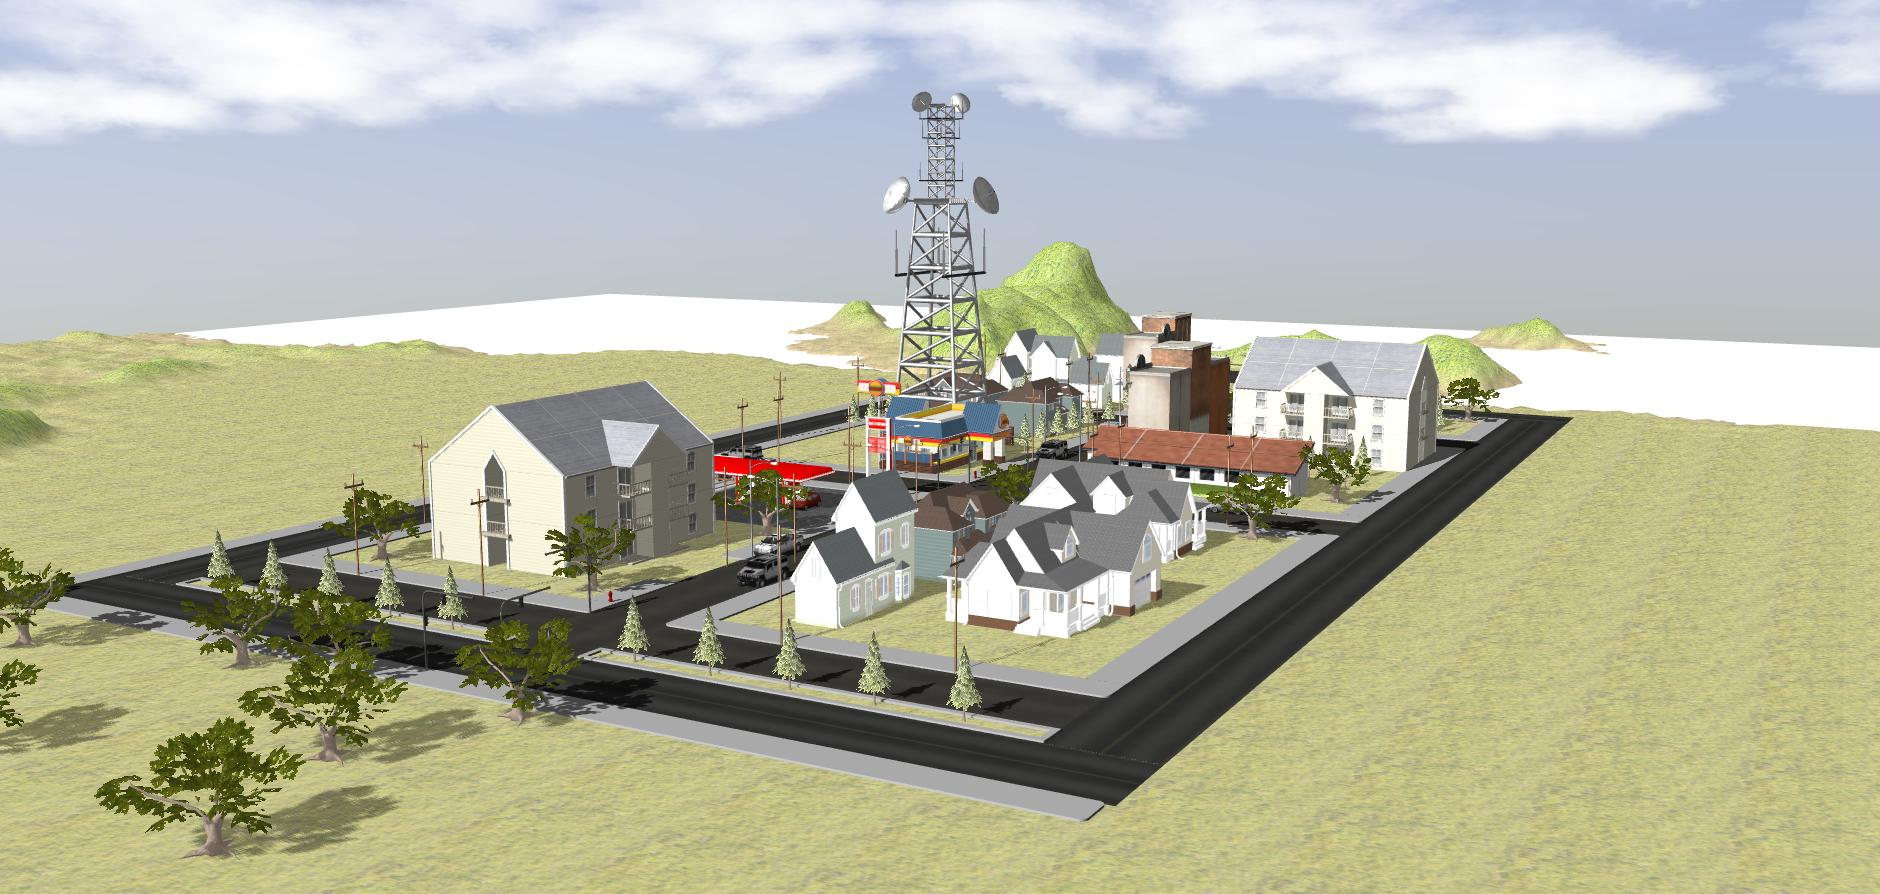
\includegraphics[width=7cm]{figs/city2}\hspace{1cm}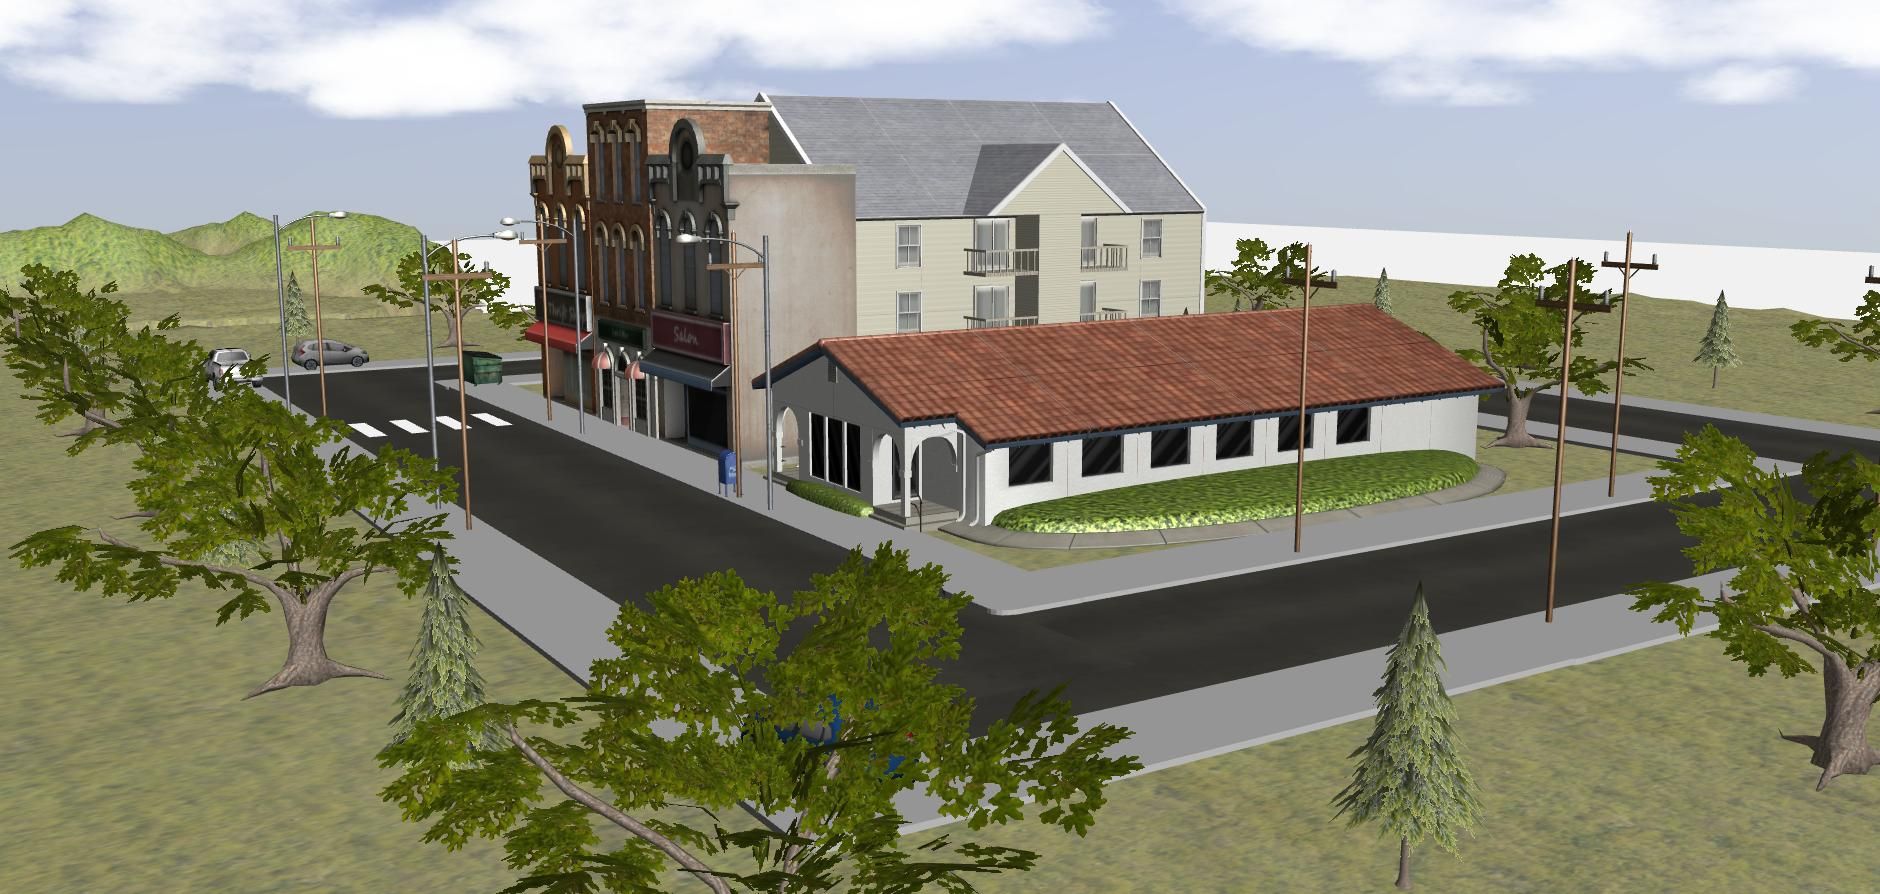
\includegraphics[width=7cm]{figs/smallcity}
	\end{center}
	\caption{Modelo de la ciudad original y la ciudad modificada en \textit{Gazebo}.}
	\label{fig:cityversus}
\end{figure}\

El modelo de esta ciudad es estático, es decir, no contiene elementos dinámicos, por lo que es necesario añadir dos tipos de elementos; un semáforo y un peatón que cruce un paso de peatones. Para ello, es necesario añadir dos \textit{plugins} para \textit{Gazebo}. En primer lugar, y usando un modelo \textit{SDF} que integra el \textit{plugin} de cambio de color en el semáforo\footnote{\url{https://github.com/robustify/gazebo_traffic_light}}. Dicho \textit{plugin} tiene asociado un fichero de configuración en formato \textit{YAML}, Código \ref{cod:trafficlight}, en el que se especifica la secuencia de estados del semáforo y su duración en el tiempo.\\

\begin{code}[h]
	\begin{lstlisting}
		light_sequence:
  - { color: "green", duration: 10, flashing: false }
  - { color: "yellow", duration: 1, flashing: false }
  - { color: "red", duration: 50, flashing: false }
	\end{lstlisting}
	\caption[Definición de estados y duraciones del semáforo.]{Definición de estados y duraciones del semáforo.}
	\label{cod:trafficlight}
\end{code}

El segundo \textit{plugin} proporciona movimiento a un modelo de un humano llamado actor. Está disponible en otro repositorio\footnote{\url{https://github.com/BruceChanJianLe/gazebo-plugin-autonomous-actor}} de \textit{GitHub} y permite que el humano se desplace en el mundo de forma realista. El \textit{plugin} citado también permite configuración para especificar la ruta de puntos o \textit{waypoints} que el peatón ha de seguir, así como, su velocidad o la distancia mínima a la que debe situarse respecto a un obstáculo. Dicha configuración se realiza directamente en el fichero \textit{SDF}, como muestra el Código \ref{cod:pedestrianconfiguration}.\\

\begin{code}[h]
	\begin{lstlisting}
		<actor name="actor">
			[...]
			<plugin name="trajectory" filename="libTrajectoryActorPlugin.so">
					<target>
					2.4028 -6.9143 1.1 1.570796 -0.0 3.141593
				</target>
					<target>
					2.4028 6.6816 1.1 1.570796 -0.0 3.141593
				</target>
					<velocity>0.75</velocity>
					<obstacle_margin>1.5</obstacle_margin>
					<obstacle></obstacle>
				</plugin>
			</actor>
	\end{lstlisting}
	\caption[Configuración de \textit{waypoints}, velocidad y distancia a obstáculos del peatón.]{Configuración de \textit{waypoints}, velocidad y distancia a obstáculos del
		peatón.}
	\label{cod:pedestrianconfiguration}
\end{code}

Ambos modelos se sitúan en una paso de peatones, creado a partir de láminas blancas, produciendo el resultado de la Figura \ref{fig:trafficlightpedestrian}.\\

\begin{figure} [h!]
	\begin{center}
		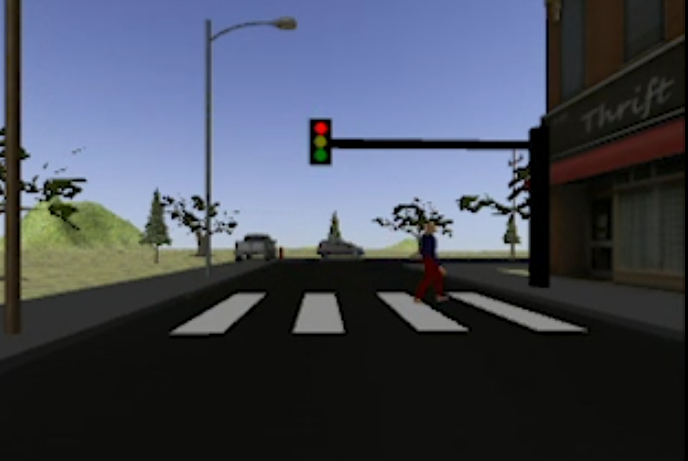
\includegraphics[width=8cm]{figs/trafficlightpedestrian}
	\end{center}
	\caption{Semáforo y peatón usando \textit{plugins} para \textit{Gazebo}.}
	\label{fig:trafficlightpedestrian}
\end{figure}\

\subsection{Modelo del coche autónomo}
\label{subsection:vehiclemodel}
El primer paso para desarrollar un modelo es diseñar las piezas a utilizar, para ello, como se explicó en el Capítulo 2, se utilizará \textit{FreeCAD}. El segundo paso es ensamblar el robot con \textit{Blender} utilizando el \textit{add-on} \textit{Phobos} para definir los \textit{links} y \textit{joints} del robot con el objetivo de dotar al robot de movimiento, generando un fichero \textit{URDF}. Por último, es necesario modificar el \textit{URDF} para añadir cámaras y controladores para los motores que serán usados en el simulador \textit{Gazebo}.\\

\subsubsection{Diseño de las piezas en \textit{FreeCAD}}

A través de la herramienta \textit{Sketcher}\footnote{\url{https://wiki.freecadweb.org/Sketcher_Workbench}}, disponible en \textit{FreeCAD}, es posible realizar un diseño de piezas en 2D con restricciones de horizontalidad, verticalidad, igualdad entre rectas, medidas, ángulos etc y después convertir dicha pieza en 3D proporcionando un volumen a la pieza. Utilizando dicha herramienta se diseña el chasis y las ruedas del vehículo tomando las medidas reales, lo que da como resultado el diseño de las piezas en 2D de la Figura \ref{fig:design2Dfreecad}.\\

\begin{figure} [h!]
	\begin{center}
		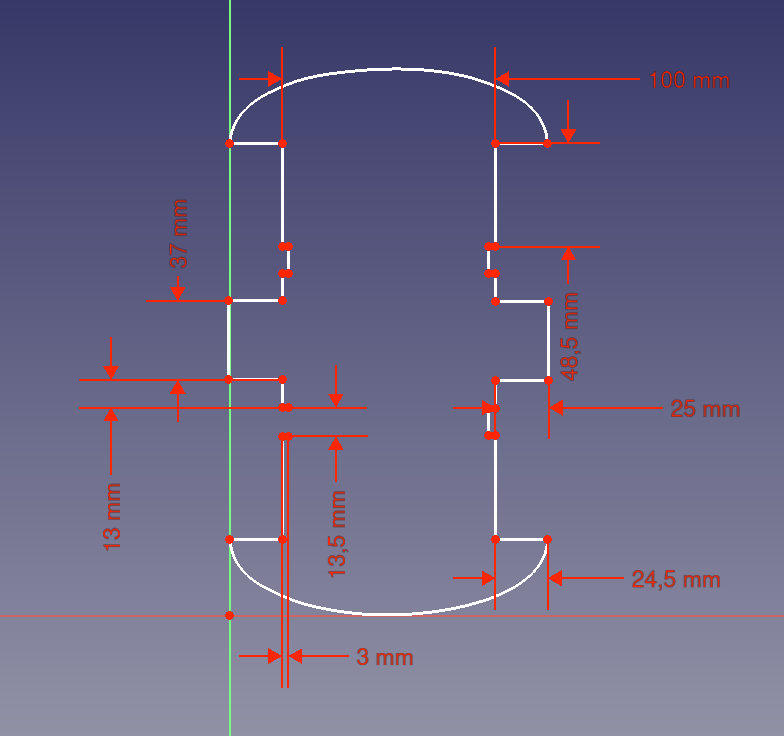
\includegraphics[width=8cm]{figs/sketchFreecad}
	\end{center}
	\caption{Diseño del chasis 2D en \textit{FreeCAD}.}
	\label{fig:design2Dfreecad}
\end{figure}\

A continuación se proporciona un grosor al chasis de 3mm y a las ruedas de xmm, obteniendo el modelo 3D de la Figura \ref{fig:design3Dfreecad}.\\

\begin{figure} [h!]
	\begin{center}
		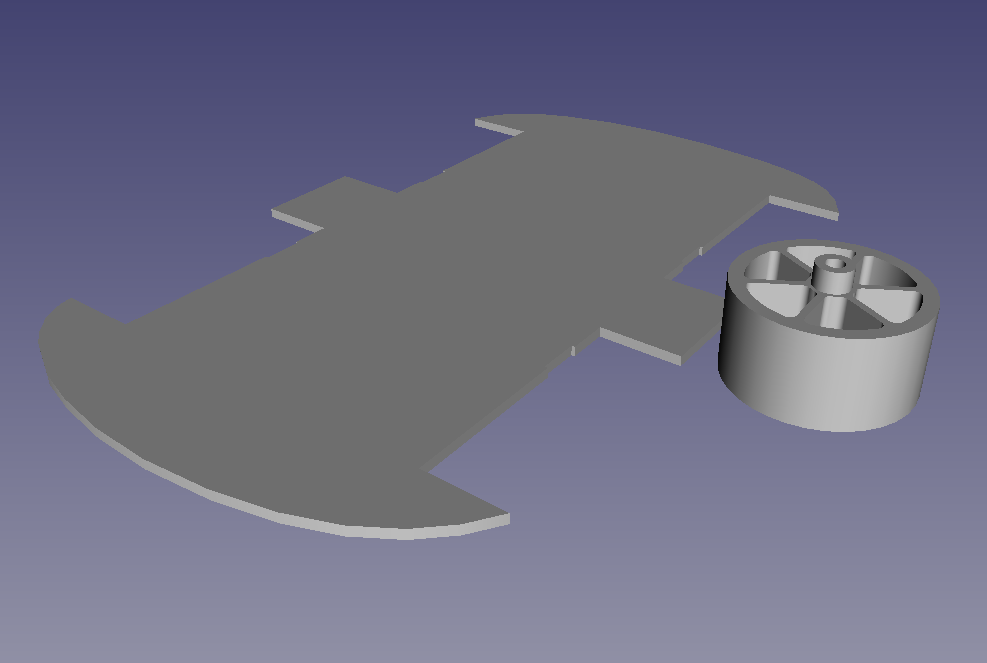
\includegraphics[width=8cm]{figs/freecad}
	\end{center}
	\caption{Diseño de las piezas 3D en \textit{FreeCAD}.}
	\label{fig:design3Dfreecad}
\end{figure}\

El siguiente paso es exportar las piezas diseñadas en formato \textit{STL} para utilizarlas en \textit{Blender}.\\

\subsubsection{Ensamblado del robot en \textit{Blender}}

Una vez importadas las piezas diseñadas en \textit{FreeCAD}, se crean dos unidades del chasis y cuatro ruedas, a continuación se mueven y rotan en el espacio para situarlas correctamente. Con el objetivo de dotar de mayor realismo al modelo, se importan modelos de los motores y la placa utilizados, disponibles en y en. Y se diseñan dos piezas para emular la batería y la cámara del robot. Con todo ello se conforma el modelo estático del robot, Figura \ref{fig:blendermodel}.\\

\begin{figure} [h!]
	\begin{center}
		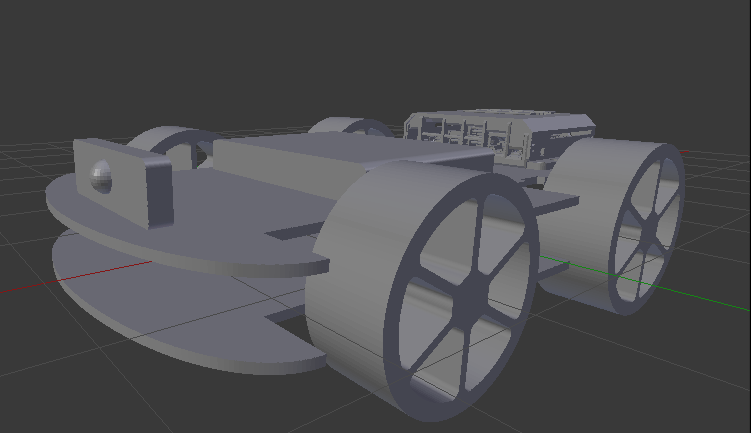
\includegraphics[width=8cm]{figs/blenderModel}
	\end{center}
	\caption{Modelo 3D estático ensamblado en \textit{Blender}.}
	\label{fig:blendermodel}
\end{figure}\

Este modelo es estático, es decir, no es posible simular un movimiento. Para ello es necesario un \textit{add-on} para \textit{Blender} como \textit{Phobos}, que como se explicó anteriormente, permite crear \textit{links} y \textit{joints} y definir una jerarquía entre ellos.\\

En primer lugar, es necesario definir los elementos visuales que compondrán el modelo, en este caso serán todas las piezas del robot, dichas piezas serán del tipo \textit{mesh}, ya que no son objetos primitivos, como cajas o esferas.\\

A continuación, se define un \textit{link} principal que será el cuerpo del robot, de este \textit{link} dependerán las cuatro ruedas del vehículo. Con el objetivo de simular colisiones, se crea un modelo de colisión de cada una de las piezas y un modelo inercial, que estará relacionado con el peso simulado de cada pieza.\\

Por último, se definen los \textit{joints} de cada rueda. A través de está funcionalidad es posible aplicar fuerza o velocidad a las ruedas del robot. Existen diferentes tipos de
\textit{joints} en \textit{Phobos}; \textit{fixed}, \textit{revolute}, \textit{continuous}, \textit{prismatic}, en este caso, son necesarios \textit{joints} de tipo \textit{continuous}, ya que las ruedas realizan un giro sin un límite fijado, y no un movimiento transversal.\\

Una vez definidos todos los elementos del modelo y su jerarquía, en el menú lateral de \textit{Blender} se encontrará el diagrama del modelo, Figura \ref{fig:blenderdiagram}.\\

\begin{figure} [h!]
	\begin{center}
		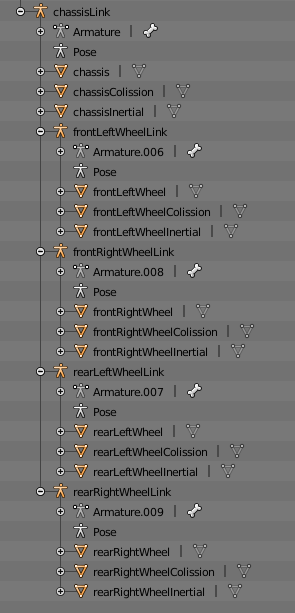
\includegraphics[width=6cm]{figs/phobosDiagram}
	\end{center}
	\caption{Diagrama del modelo diseñado con \textit{Phobos}.}
	\label{fig:blenderdiagram}
\end{figure}\

El siguiente paso es exportar el modelo a formato \textit{URDF}, que como se explicó anteriormente, es el aceptado por \textit{Gazebo} para simular modelos de robots. Las mallas, que componen el modelo visual y de colisiones, se exportan en formato \textit{DAE}, y se cargan desde el modelo \textit{URDF}.\\

\subsubsection{Adición de plugins para \textit{Gazebo}}

Con el objetivo de mover el robot utilizando el \textit{middleware ROS}, es necesario cargar el \textit{plugin} \textit{Gazebo ROS Control} mediante el Código \ref{cod:gazeboroscontrol}.\\

\begin{code}[h]
	\begin{lstlisting}[language=XML]
		<gazebo>
		<plugin name="gazebo_ros_control" filename="libgazebo_ros_control.so">
			<robotNamespace>/autonomous_vehicle</robotNamespace>
		</plugin>
		</gazebo>
	\end{lstlisting}
	\caption[Carga del \textit{plugin} \textit{Gazebo ROS Control}.]{Carga del \textit{plugin} \textit{Gazebo ROS Control}.}
	\label{cod:gazeboroscontrol}
\end{code}

Otro elemento a añadir en el fichero \textit{URDF}, es la existencia de dos cámaras; una cámara \textit{onboard} y otra situada encima del robot que proporcionará una visión de la ruta realizada. Dichas cámaras simuladas publicarán su imagen en un \textit{topic} de \textit{ROS} con una resolución y un formato fijado mediante el Código \ref{cod:gazebocamera}.\\

\begin{code}[h]
	\begin{lstlisting}[language=XML]
	<gazebo reference="onboardCameraLink">
		<sensor name='cam_sensor' type='camera'>
			[...]
			<camera name='onboardCameraLink'>
				<horizontal_fov>1.570000</horizontal_fov>
				<image>
					<width>320</width>
					<height>240</height>
					<format>R8G8B8</format>
				</image>
				[...]
			</camera>
			[...]
		</sensor>
	</gazebo>
	\end{lstlisting}
	\caption[Crear cámara simulada en \textit{Gazebo}.]{Crear cámara simulada en \textit{Gazebo}.}
	\label{cod:gazebocamera}
\end{code}

Para mover el robot simulado también será necesario un fichero \textit{YAML}, en el que se especifiquen los controladores de los \textit{joints} y el nombre de los \textit{topics} en los que se publicarán los mensajes mediante el Código \ref{cod:controllers}.\\

\begin{code}[h]
	\begin{lstlisting}
		autonomous_vehicle:
		joint_state_controller:
			type: joint_state_controller/JointStateController
			publish_rate: 10
		front_right_wheel_velocity_controller:
			type: velocity_controllers/JointVelocityController
			joint: frontRightWheelJoint
		front_left_wheel_velocity_controller:
			type: velocity_controllers/JointVelocityController
			joint: frontLeftWheelJoint
		rear_right_wheel_velocity_controller:
			type: velocity_controllers/JointVelocityController
			joint: rearRightWheelJoint
		rear_left_wheel_velocity_controller:
			type: velocity_controllers/JointVelocityController
			joint: rearLeftWheelJoint
	\end{lstlisting}
	\caption[Definición de los controladores de los \textit{joints} del robot.]{Definición de los controladores de los \textit{joints} del robot.}
	\label{cod:controllers}
\end{code}

Con todo ello, se implementa un \textit{launcher}\footnote{\url{https://github.com/jmvega/tfg-amariscal/src/launcher......}} que lanza el modelo dińamico del robot y se muestra en la ciudad simulada tal y como se representa en la Figura \ref{fig:modelGazebo}.\\

\begin{figure} [h!]
	\begin{center}
		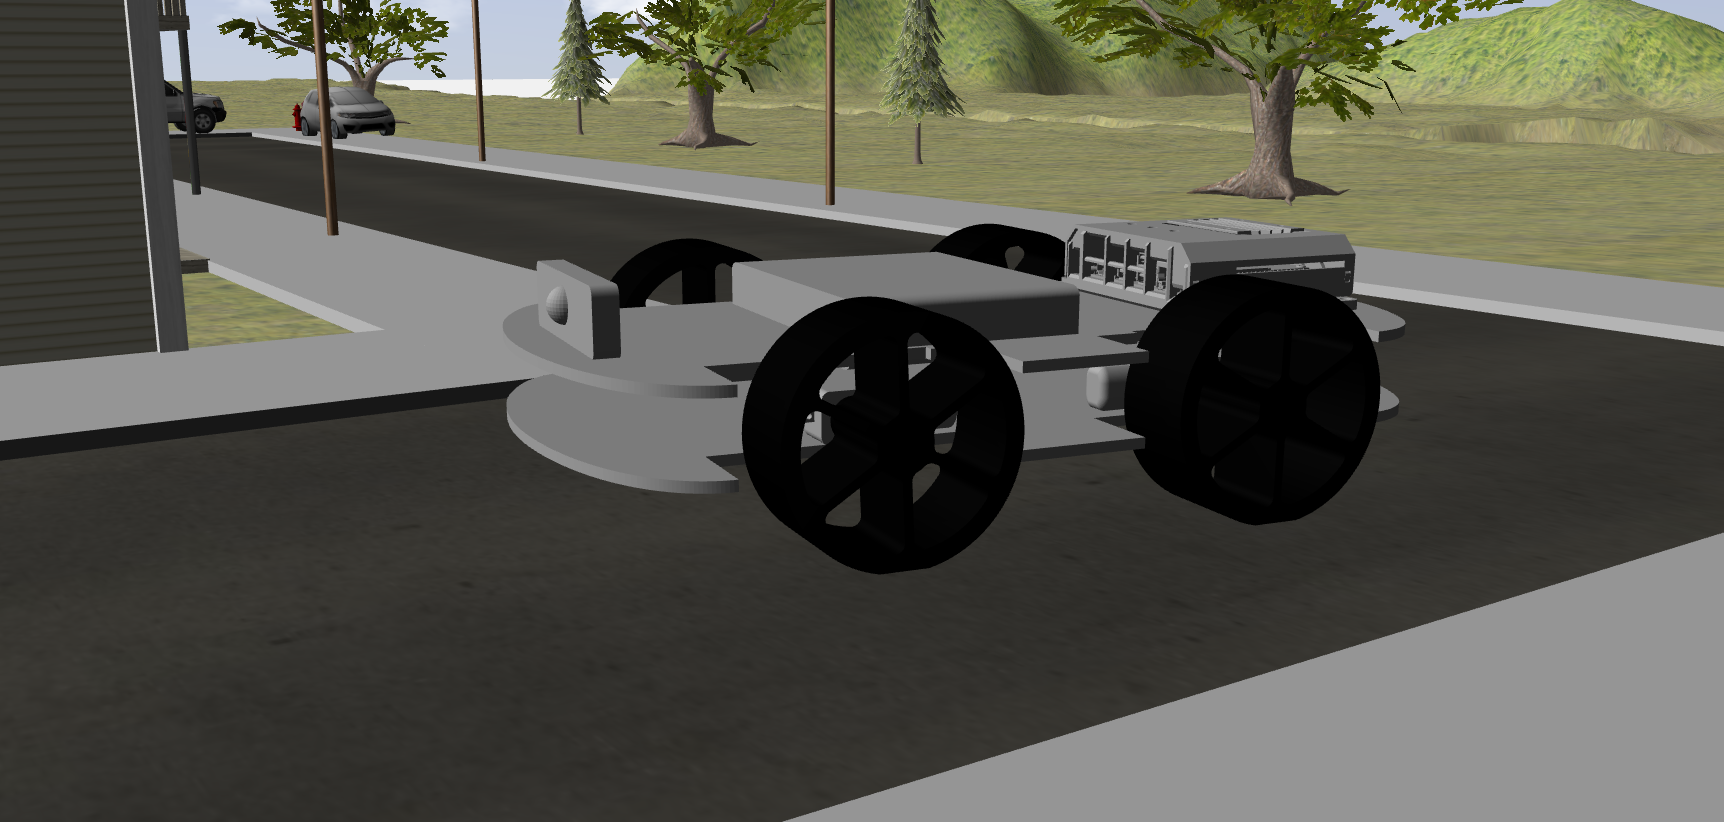
\includegraphics[width=12cm]{figs/modelGazebo}
	\end{center}
	\caption{Modelo dinámico del robot en \textit{Gazebo}.}
	\label{fig:modelGazebo}
\end{figure}\

\subsection{Seguimiento de carril}
\label{subsection:lanefollower}
\footnote{\url{https://github.com/jmvega/tfg-amariscal/src/......... interactive_regression_ros}}
Como se explicó en el Capítulo 2, la biblioteca elegida para realizar el seguimiento de carril, es \textit{JetRacer} tal y como se expuso en la Sección \ref{subsection:jetracer}. Dicha biblioteca se basa en la utilización de una red \textit{ResNet-18} preentrenada, consistente en una red neuronal convolucional de 18 capas, sobre la que a su vez, se entrena con un \textit{dataset} de un escaso mínimo número de imágenes. Proporciona diversos \textit{notebooks} de \textit{Jupyter} que hacen más la sencilla la obtención del \textit{dataset}, el entrenamiento y el ajuste del controlador.\\

El primer paso es la obtención del \textit{dataset} para posteriormente entrenar la red. Para ello, es necesario asociar cada imagen con el centro del carril, definido a partir de una coordenada en x y otra en y. La librería utiliza un \textit{widget} para \textit{Jupyter} llamado \textit{Jupyter Clickable Image Widget\footnote{\url{https://github.com/jaybdub/jupyter_clickable_image_widget}}} lo que permite que al hacer click sobre la imagen recibida a partir de un flujo de vídeo, esta se guarde con un nombre atendiendo al siguiente formato: \textit{x\_y\_identificador\_unico.jpg}. Es importante entrenar también con imágenes donde el ángulo del giro del robot sea elevado, tal y como muestra la Figura \ref{fig:traineddifficult} ya que de esa forma el robot sabrá reaccionar ante situaciones difíciles.\\

\begin{figure} [h!]
	\begin{center}
		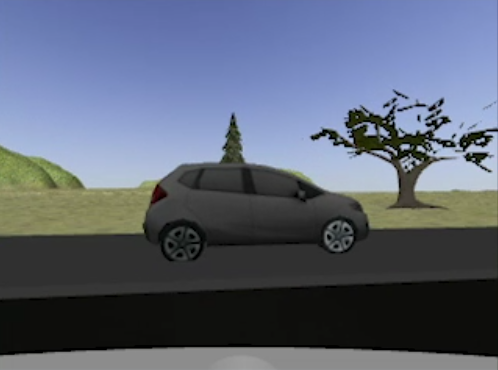
\includegraphics[width=6cm]{figs/trainedDifficult}
	\end{center}
	\caption{Imagen del \textit{dataset} donde el ángulo de giro necesario es elevado.}
	\label{fig:traineddifficult}
\end{figure}\

Para mover el robot dentro del simulador es necesario utilizar los controladores de los motores anteriormente desarrollados y para mayor comodidad, se realizó un control manual a través de una interfaz con \textit{PyQT} que se detallará en la Sección \ref{subsection:interface}.\\

Una vez obtenido el \textit{dataset}, se descarga el modelo preentrenado \textit{ResNet-18} utilizando la librería \textit{Torchvision} y se realiza una conversión para aprovechar los núcleos de la tarjeta gráfica mediante la plataforma \textit{CUDA} a través de la función \verb|to(device)| donde \verb|device| es \verb|torch.device('cuda')|.\\

El siguiente paso es el entrenamiento de la red. Para ello, en cada \textit{epoch} se calcula el error cuadrático medio, \textit{mean squared error (MSE loss)} entre una de las imágenes del \textit{dataset} y la salida actual de la red. Una vez calculado este error se realiza la propagación hacia detrás, \textit{backpropagation}, consistente en la propagación de los errores desde la capa de salida hasta la primera capa. Además se realiza una optimización de los pesos a través del algoritmo \textit{Adam} \cite{adam}, el cual es un método de optimización estocástica basado en el cálculo de las tasas individuales adaptables de entrenamiento, \textit{individual adaptive learning rates} a partir de estimaciones del primer y segundo momento del gradiente.\\

Para realizar el entrenamiento hay que fijar un número de \textit{epochs} que será el momento en el que el entrenamiento finalizará. En cada \textit{epoch} el error va bajando hasta llegar a un valor cercano a 0, dependiendo del número de imágenes del \textit{dataset} el tiempo invertido en realizar una \textit{epoch} será mayor o menor. En el caso del entrenamiento realizado, en 10 \textit{epochs} el error alcanzó el valor de 0.0117 tal y como representa la Figura \ref{fig:epochsimulator}.\\

\begin{figure} [h!]
	\begin{center}
		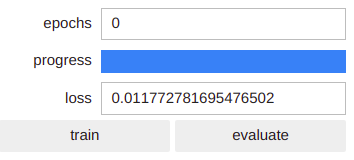
\includegraphics[width=8cm]{figs/epochSimulator}
	\end{center}
	\caption{Valor del error al finalizar el entrenamiento en el entorno simulado.}
	\label{fig:epochsimulator}
\end{figure}\

Tanto el entrenamiento como la ejecución de la red neuronal recibe imágenes de una baja resolución, 240 píxeles, ya que está diseñada para funcionar en placas de bajas prestaciones. Tras realizar el entrenamiento se genera un modelo \textit{.pth}. Para poder obtener la salida de la red es necesario pasar como argumento al modelo, el resultado de la función \verb|preprocess(image)|, que devuelve un tensor a partir de una imagen en formato \verb|numpy.ndarray|, tal y como se observa en el Código \ref{cod:lane}. Tras obtener la salida es posible representar el centro del carril con el resultado de la Figura \ref{fig:outputnnsim}.\\

\begin{code}[h]
	\begin{lstlisting}[language=Python]
			image = camera.read()
    		preprocessed = preprocess(image)
    		output = model(preprocessed).detach().cpu().numpy().flatten()
	\end{lstlisting}
	\caption[Obtención de la salida de la red neuronal \textit{ResNet-18}.]{Obtención de la salida de la red neuronal \textit{ResNet-18}.}
	\label{cod:lane}
\end{code}

\begin{figure} [h!]
	\begin{center}
		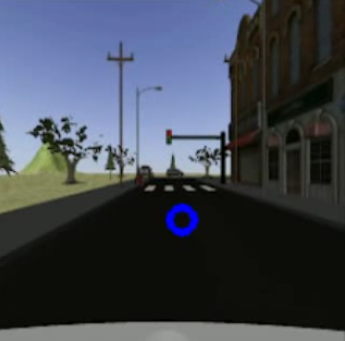
\includegraphics[width=6cm, height=5cm]{figs/outputNNsim}
	\end{center}
	\caption{Salida de la red neuronal \textit{ResNet-18} en el simulador \textit{Gazebo}.}
	\label{fig:outputnnsim}
\end{figure}\

En el caso del simulador y al ser una plataforma de pruebas, el objetivo principal es entrenar la red y probar su efectividad en un entorno simulado, y no desarrollar un controlador a partir de la salida de la red. Por lo que el seguimiento del carril se realizará mediante un autómata que recorrerá la ciudad de forma que se pueda observar el comportamiento de la red neuronal.\\

\subsection{Detección de objetos}
\label{subsection:objectdetector}
La detección de objetos se ha llevado a cabo mediante una red neuronal convolucional llamada \textit{YOLO V3 Tiny} debido a su gran rendimiento en placas de reducida potencia. La versión \textit{Tiny-YOLO} reduce el número de capas y precisión de detección pero aumenta la tasa de \textit{FPS} por lo que es muy conveniente su uso en dispositivos como \textit{NVIDIA Jetson Nano}. Existen distintas versiones de \textit{Tiny-YOLO}. La tercera versión cuenta con 15 capas convolucionales\footnote{\url{https://github.com/pjreddie/darknet/blob/master/cfg/yolov3-tiny.cfg}} a diferencia de la cuarta que cuenta con 29 capas\footnote{\url{https://github.com/AlexeyAB/darknet/blob/master/cfg/yolov4-tiny.cfg}}. En el Cuadro \ref{table:v3vsv4} se puede observar una comparación entre ambas versiones de la red con una resolución de 416 píxeles, extraída de la siguiente fuente\cite{versus}, que arroja como resultado un mejor rendimiento en la tercera versión, si bien es cierto que atendiendo al artículo de \textit{YOLO V4} \cite{yolov4} la precisión de la red ha sido incrementada en un 10\% en decremento de la tasa de \textit{FPS}.\\

\begin{table}[H]
	\begin{center}
		\begin{tabular}{|c|c|c|}
			\hline
			\textbf{Placa}     & \textbf{YOLO V3 Tiny} & \textbf{YOLO V4 Tiny}
			\\
			\hline
			NVIDIA Jetson Nano & 15                    & 7.8
			\\
			NVIDIA Jetson TX2  & 19                    & 11.5
			\\
			NVIDIA AGX Xavier  & 32                    & 22
			\\
			\hline
		\end{tabular}
		\caption{\textit{FPS} obtenidos en diferentes placas \textit{NVIDIA}}
		\label{table:v3vsv4}
	\end{center}
\end{table}

La ejecución de la simulación se ha realizado utilizando una tarjeta gráfica \textit{NVIDIA MX330}. Se trata de una tarjeta de gama baja y consumo reducido diseñada para portátiles. En cuanto a la decisión de la resolución de la imagen con la que trabaja la red neuronal se ha realizado una comparación disponible en el Cuadro \ref{table:versusnotebook}.\\

\begin{table}[H]
	\begin{center}
		\begin{tabular}{|c|c|}
			\hline
			\textbf{Resolución} & \textbf{FPS}
			\\
			\hline
			416 x 416           & 41.1
			\\
			608 x 608           & 21.6
			\\
			832 x 832           & 12.3
			\\
			\hline
		\end{tabular}
		\caption{FPS obtenidos en \textit{YOLO V3 Tiny} con la tarjeta gráfica \textit{NVIDIA MX330}}
		\label{table:versusnotebook}
	\end{center}
\end{table}

Se ha utilizado la red \textit{YOLO V3 Tiny} sobre \textit{Darknet ROS\footnote{\url{https://github.com/leggedrobotics/darknet_ros}}}. Se trata de un paquete que implementa \textit{Darknet} utilizando el \textit{framework ROS}. Su funcionamiento se basa en la recepción de la imagen a través de un \textit{topic} fijado en el fichero de configuración \textit{ros.yaml} y la publicación de objetos detectados mediante \textit{bounding boxes} en un \textit{topic} llamado \textit{/darknet\_ros/bounding\_boxes} en el que se publican mensajes con los datos del Código \ref{cod:boundingboxes}. De esa forma se puede extraer las coordenadas del \textit{bounding box}, el objeto detectado y su probabilidad. Existe un fichero \textit{YAML} en el que se especifican los objetos a detectar y en el que es necesario especificar límite o \textit{threshold} debajo del cual el objeto detectado será descartado. En el caso del entorno simulado los colores son fijos y los objetos son muy genéricos por lo que el \textit{threshold} se pudo subir hasta 0.8. De esta forma se evitan falsos positivos y se consigue una detección mucho más fiable.\\

\begin{code}[h]
	\begin{lstlisting}
		float64 probability
		int64 xmin
		int64 ymin
		int64 xmax
		int64 ymax
		int16 id
		string Class
	\end{lstlisting}
	\caption[Contenido del mensaje \textit{BoundingBox}.]{Contenido del mensaje \textit{BoundingBox}.}
	\label{cod:boundingboxes}
\end{code}

De esta forma se pueden detectar objetos como semáforos, personas o coches tal y como se puede observar en la Figura \ref{fig:darknetsimulator}.\\

\begin{figure} [h!]
	\begin{center}
		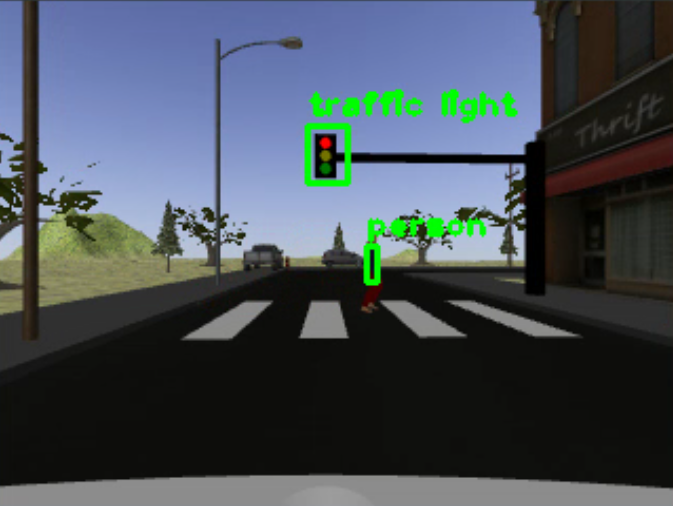
\includegraphics[width=6cm]{figs/darknetSimulator}
	\end{center}
	\caption{Salida de la red neuronal \textit{YOLO V3 Tiny} en el simulador \textit{Gazebo}.}
	\label{fig:darknetsimulator}
\end{figure}\

En el caso de la detección del semáforo es necesario tratar la imagen para detectar el color. Para ello, se extrae la imagen del \textit{bounding box} mediante sus coordenadas, contenidas en el mensaje tal y como consta en el Código \ref{cod:boundingboxes}, se transforma al espectro \textit{HSV} con el objetivo de posteriormente realizar un filtro de color. Al aplicar la máscara sobre una imagen en \textit{HSV} y no en \textit{RGB} obtenemos una detección de mayor fiabilidad, tal y como se puede observar en la Figura
\ref{fig:detector}.\\

\begin{figure} [h!]
	\begin{center}
		
\includegraphics[width=2cm, height=4cm]{figs/cropped}\hspace{2cm}
\includegraphics[width=2cm, height=4cm]{figs/hsv}\hspace{2cm}
\includegraphics[width=2cm,
			height=4cm]{figs/mask}
	\end{center}
	\caption{Detección del semáforo mediante transformación a \textit{HSV} y filtro de color.}
	\label{fig:detector}
\end{figure}\

El robot se detiene al detectar el semáforo en rojo y en el momento que cambie a verde reanuda la marcha. En el caso de detectar una señal de stop se parará durante 5 segundos.
Todo ello se puede observar en capturas de la ejecución representadas en la Figura \ref{fig:simexecution}.\\

\begin{figure} [h!]
	\begin{center}
		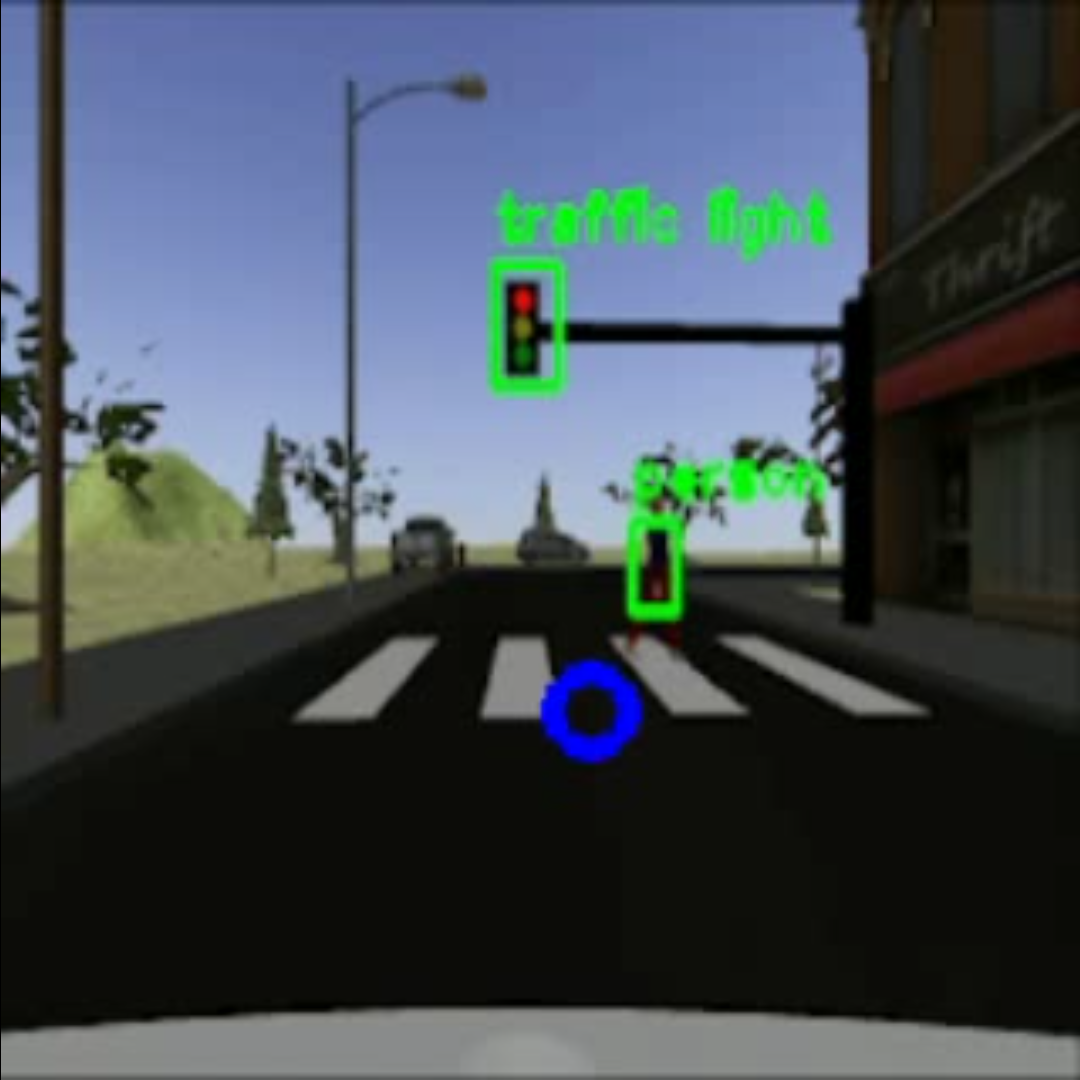
\includegraphics[width=5cm]{figs/simRed}\hspace{0.1cm}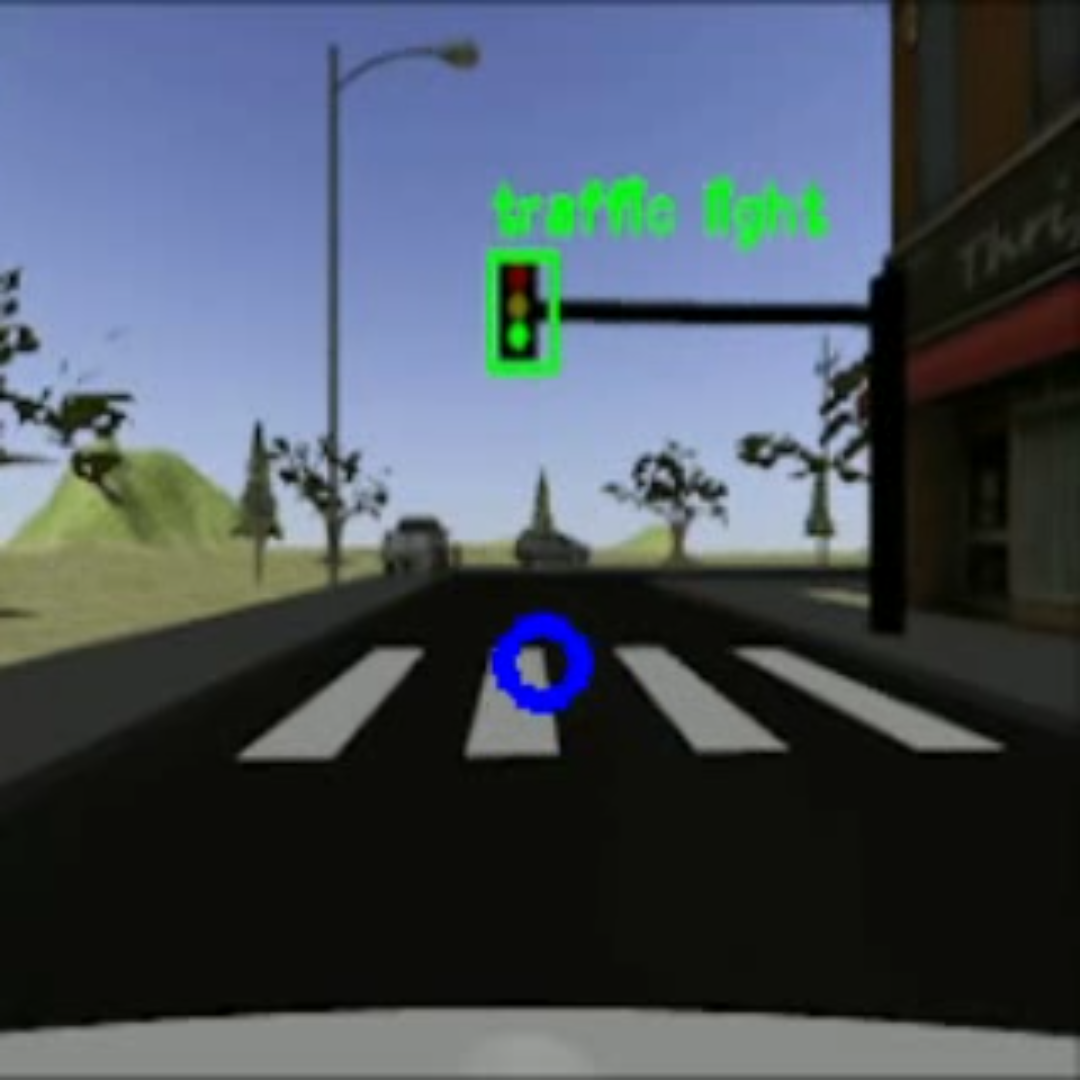
\includegraphics[width=5cm]{figs/simGreen}\hspace{0.1cm}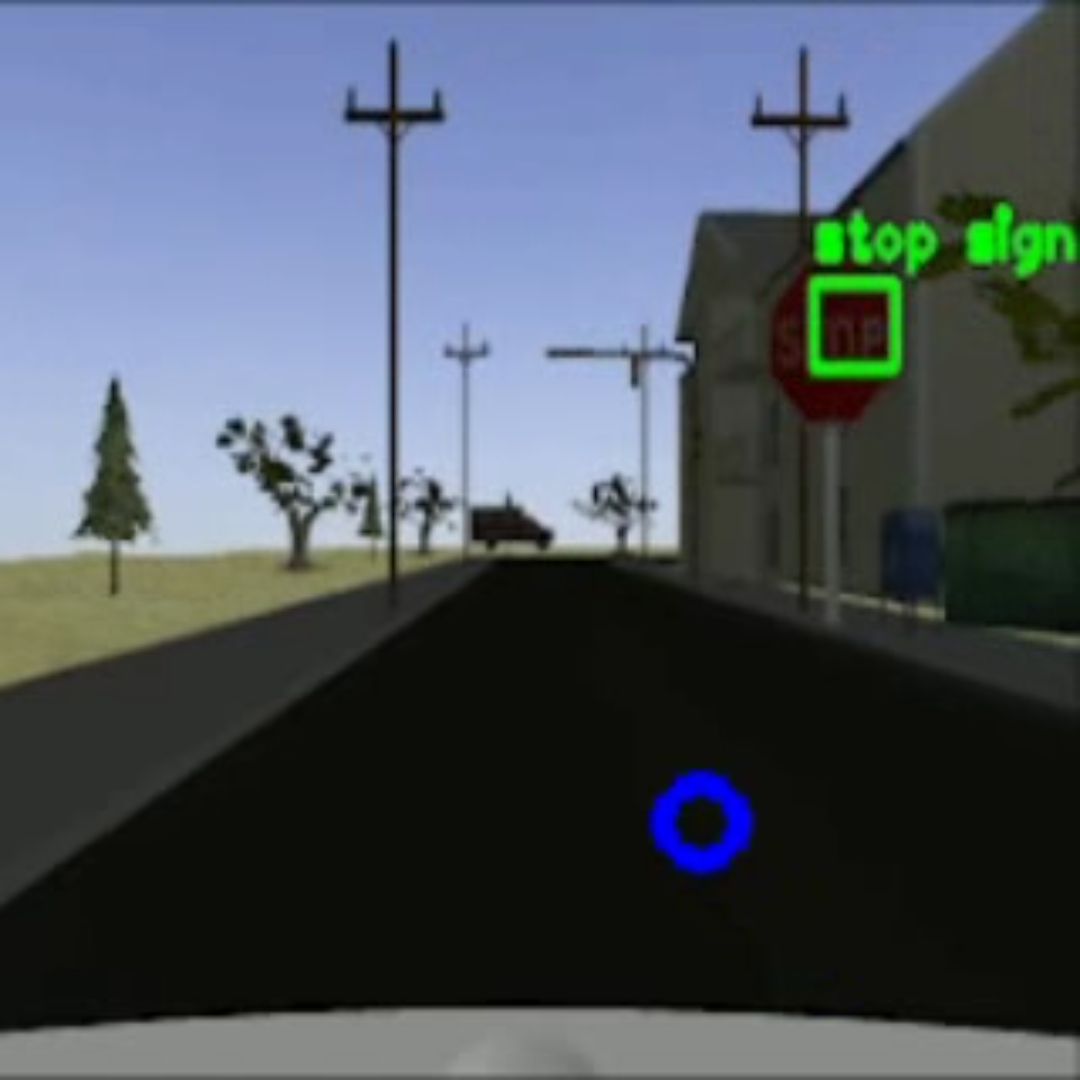
\includegraphics[width=5cm]{figs/simStop}
	\end{center}
	\caption{Capturas de la ejecución con dos redes neuronales.}
	\label{fig:simexecution}
\end{figure}\

\subsection{Interfaz de usuario}
\label{subsection:interface}
Con el objetivo de realizar un control sencillo de la simulación se ha realizado una interfaz gráfica desarrollada con la biblioteca \textit{PyQT}. Dicha interfaz dispone de una cruceta para realizar un control manual del robot. Incluye también un botón para iniciar la simulación y otro para reiniciarla, de modo que, el robot vuelve al punto inicial. Así como un botón para activar las dos cámaras. Dispone de una cámara alojada en el propio robot llamada \textit{onboard} y otra que se desplaza cuando el robot avanza de modo que aporta una visión del recorrido que realiza el robot. La interfaz descrita se puede observar en la Figura \ref{fig:gui}.\\

\begin{figure} [h!]
	\begin{center}
		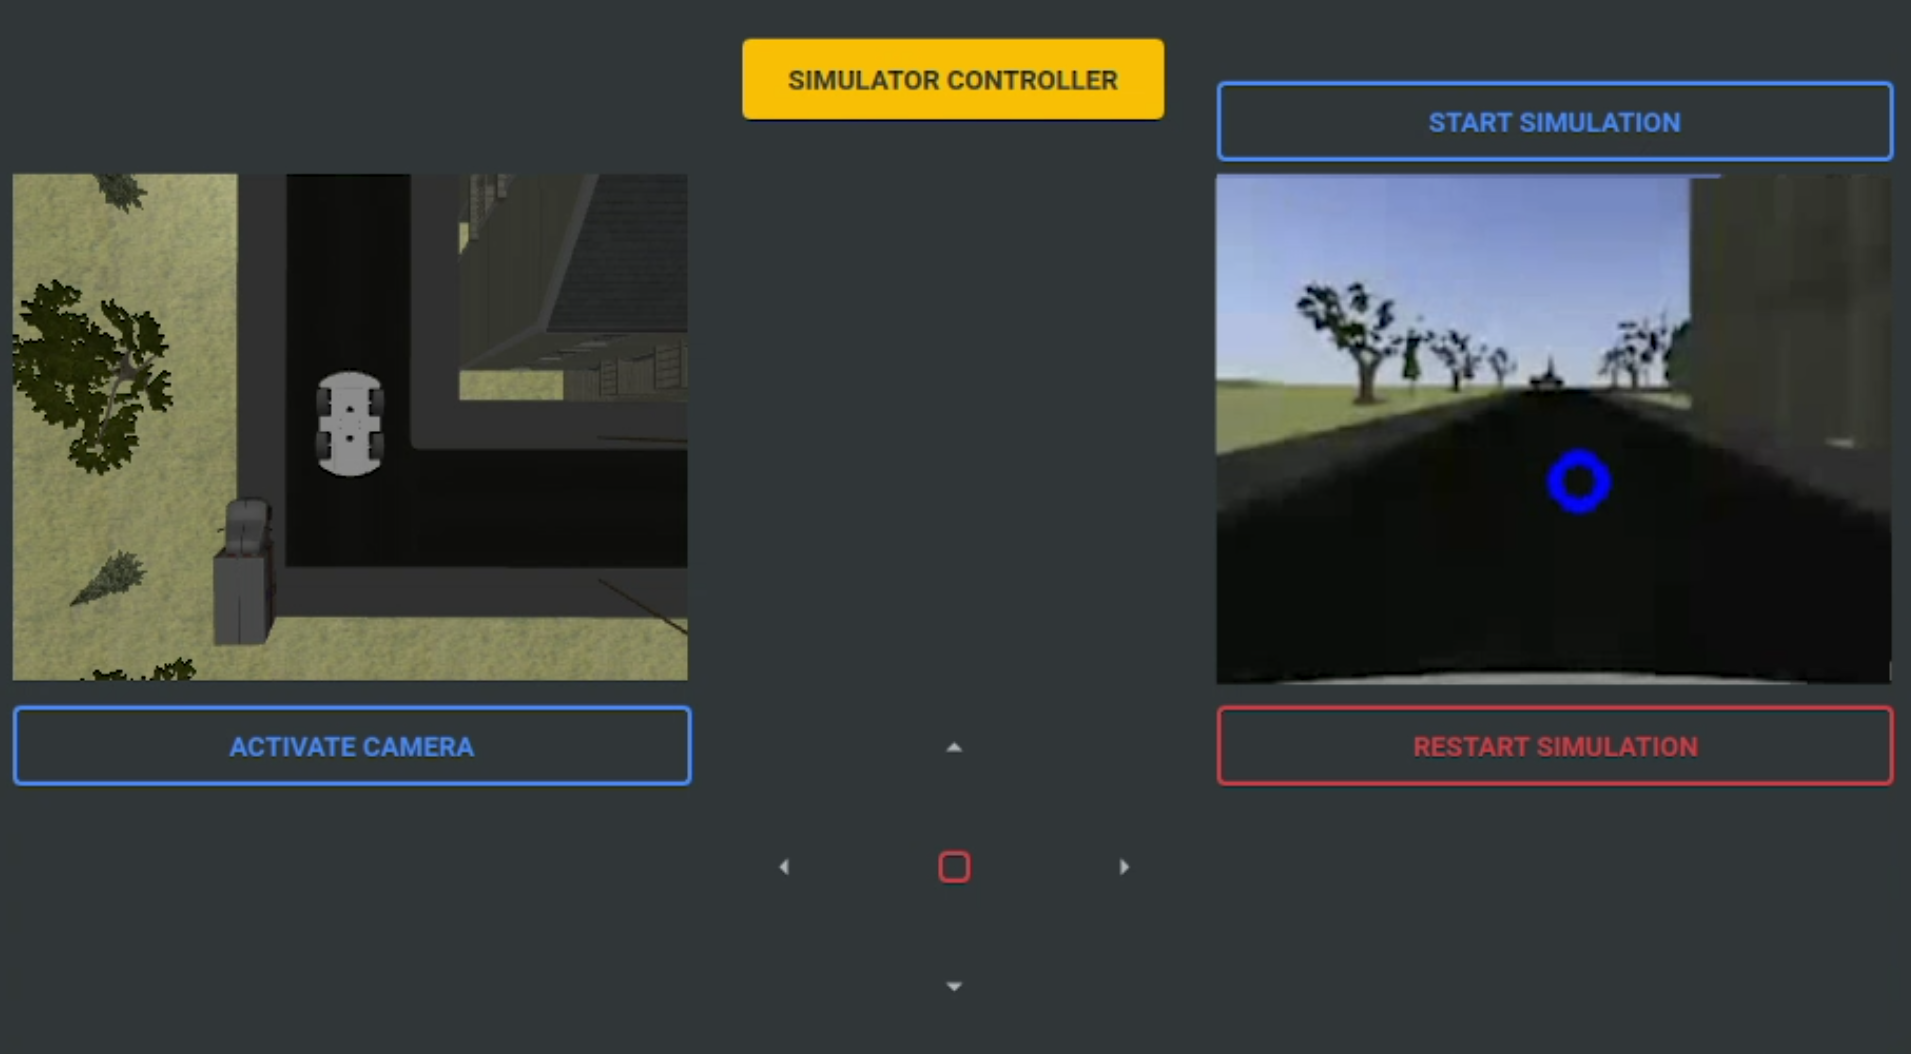
\includegraphics[width=10cm]{figs/GUI}
	\end{center}
	\caption{Interfaz de usuario desarrollada para controlar la simulación.}
	\label{fig:gui}
\end{figure}\

\section{Entorno real}
\label{section:real}
En esta sección se exponen los elementos utilizados para componer un entorno real en el que un robot, representado en la Figura \ref{fig:realrobot}, equipado con una cámara como sensor principal circula reaccionando ante objetos estáticos y dinámicos. Así como las particularidades del sistema a la hora de realizar la transición desde el entorno simulado al real.\\

\begin{figure} [h!]
	\begin{center}
		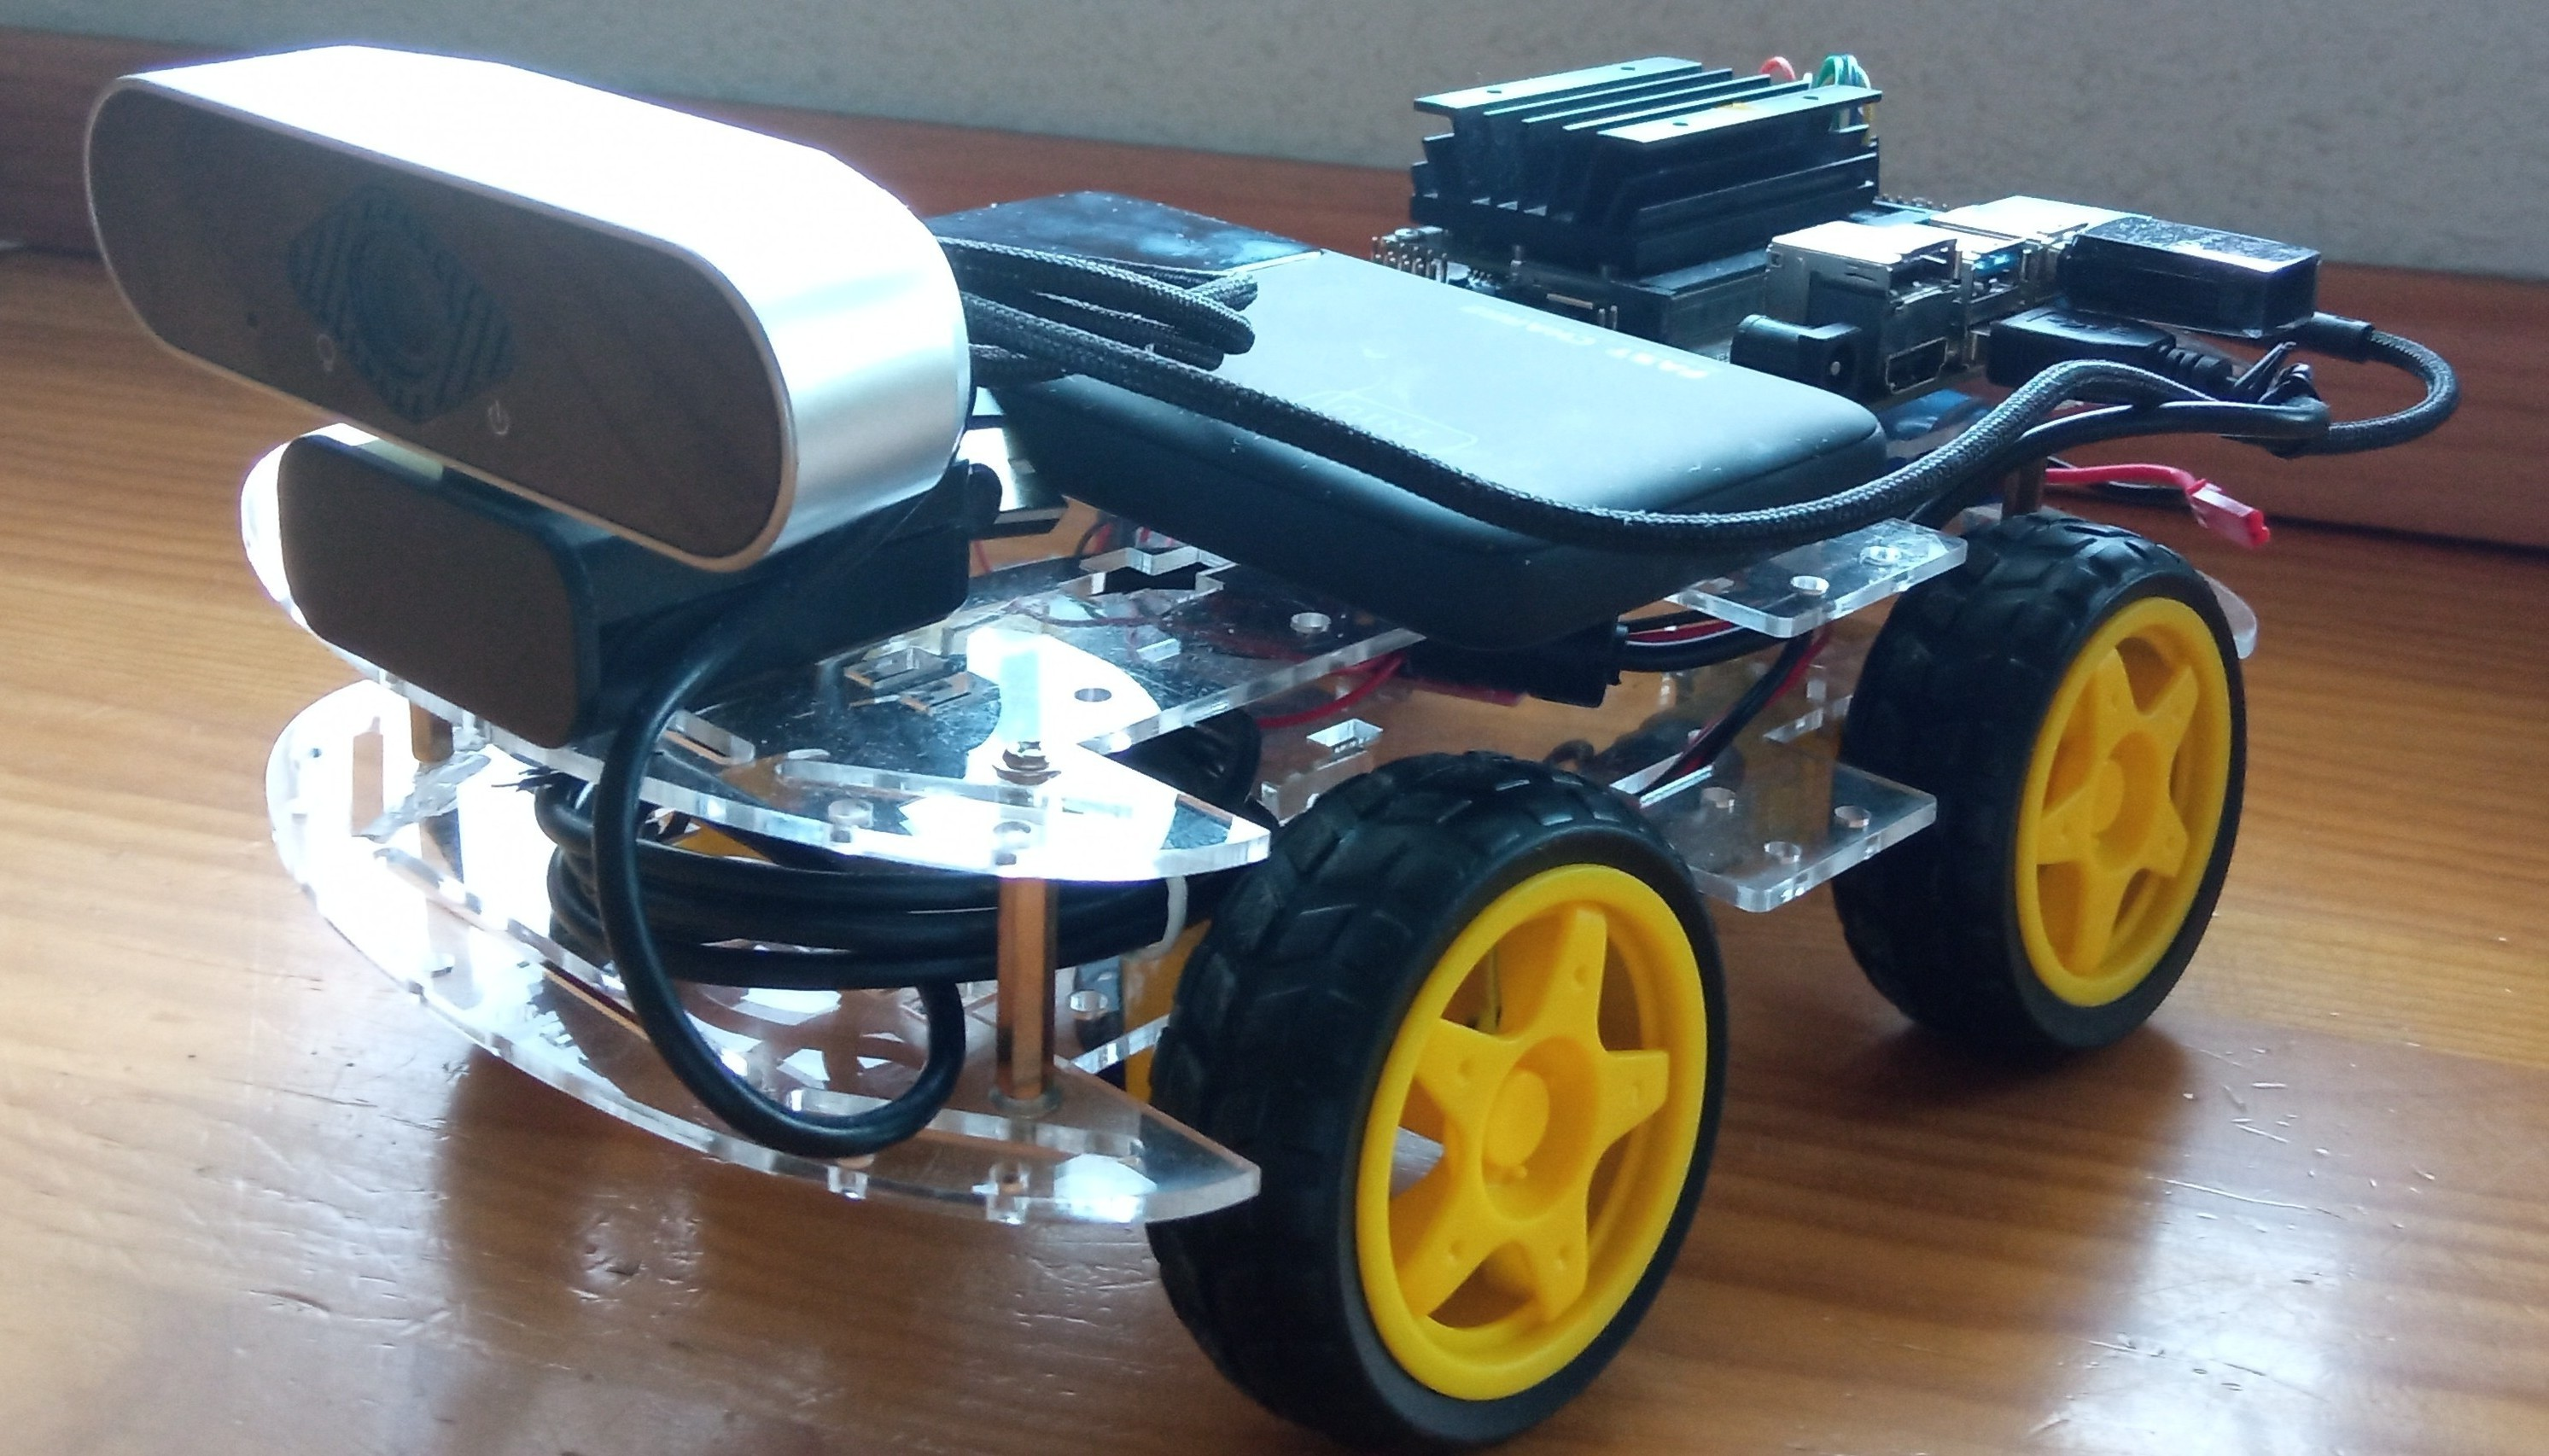
\includegraphics[width=10cm]{figs/robot}
	\end{center}
	\caption{Robot con \textit{NVIDIA Jetson Nano}.}
	\label{fig:realrobot}
\end{figure}\

\subsection{Objetos}
El entorno real se compone de diversos objetos; un circuito elaborado con pistas Scalextric sobre el que se sitúan objetos como un semáforo dinámico que cambia de color en un modo automático cada cierto tiempo, una señal de stop y un peatón. Dichos objetos se pueden observar en la Figura \ref{fig:objects}.\\

\begin{figure} [h!]
	\begin{center}
		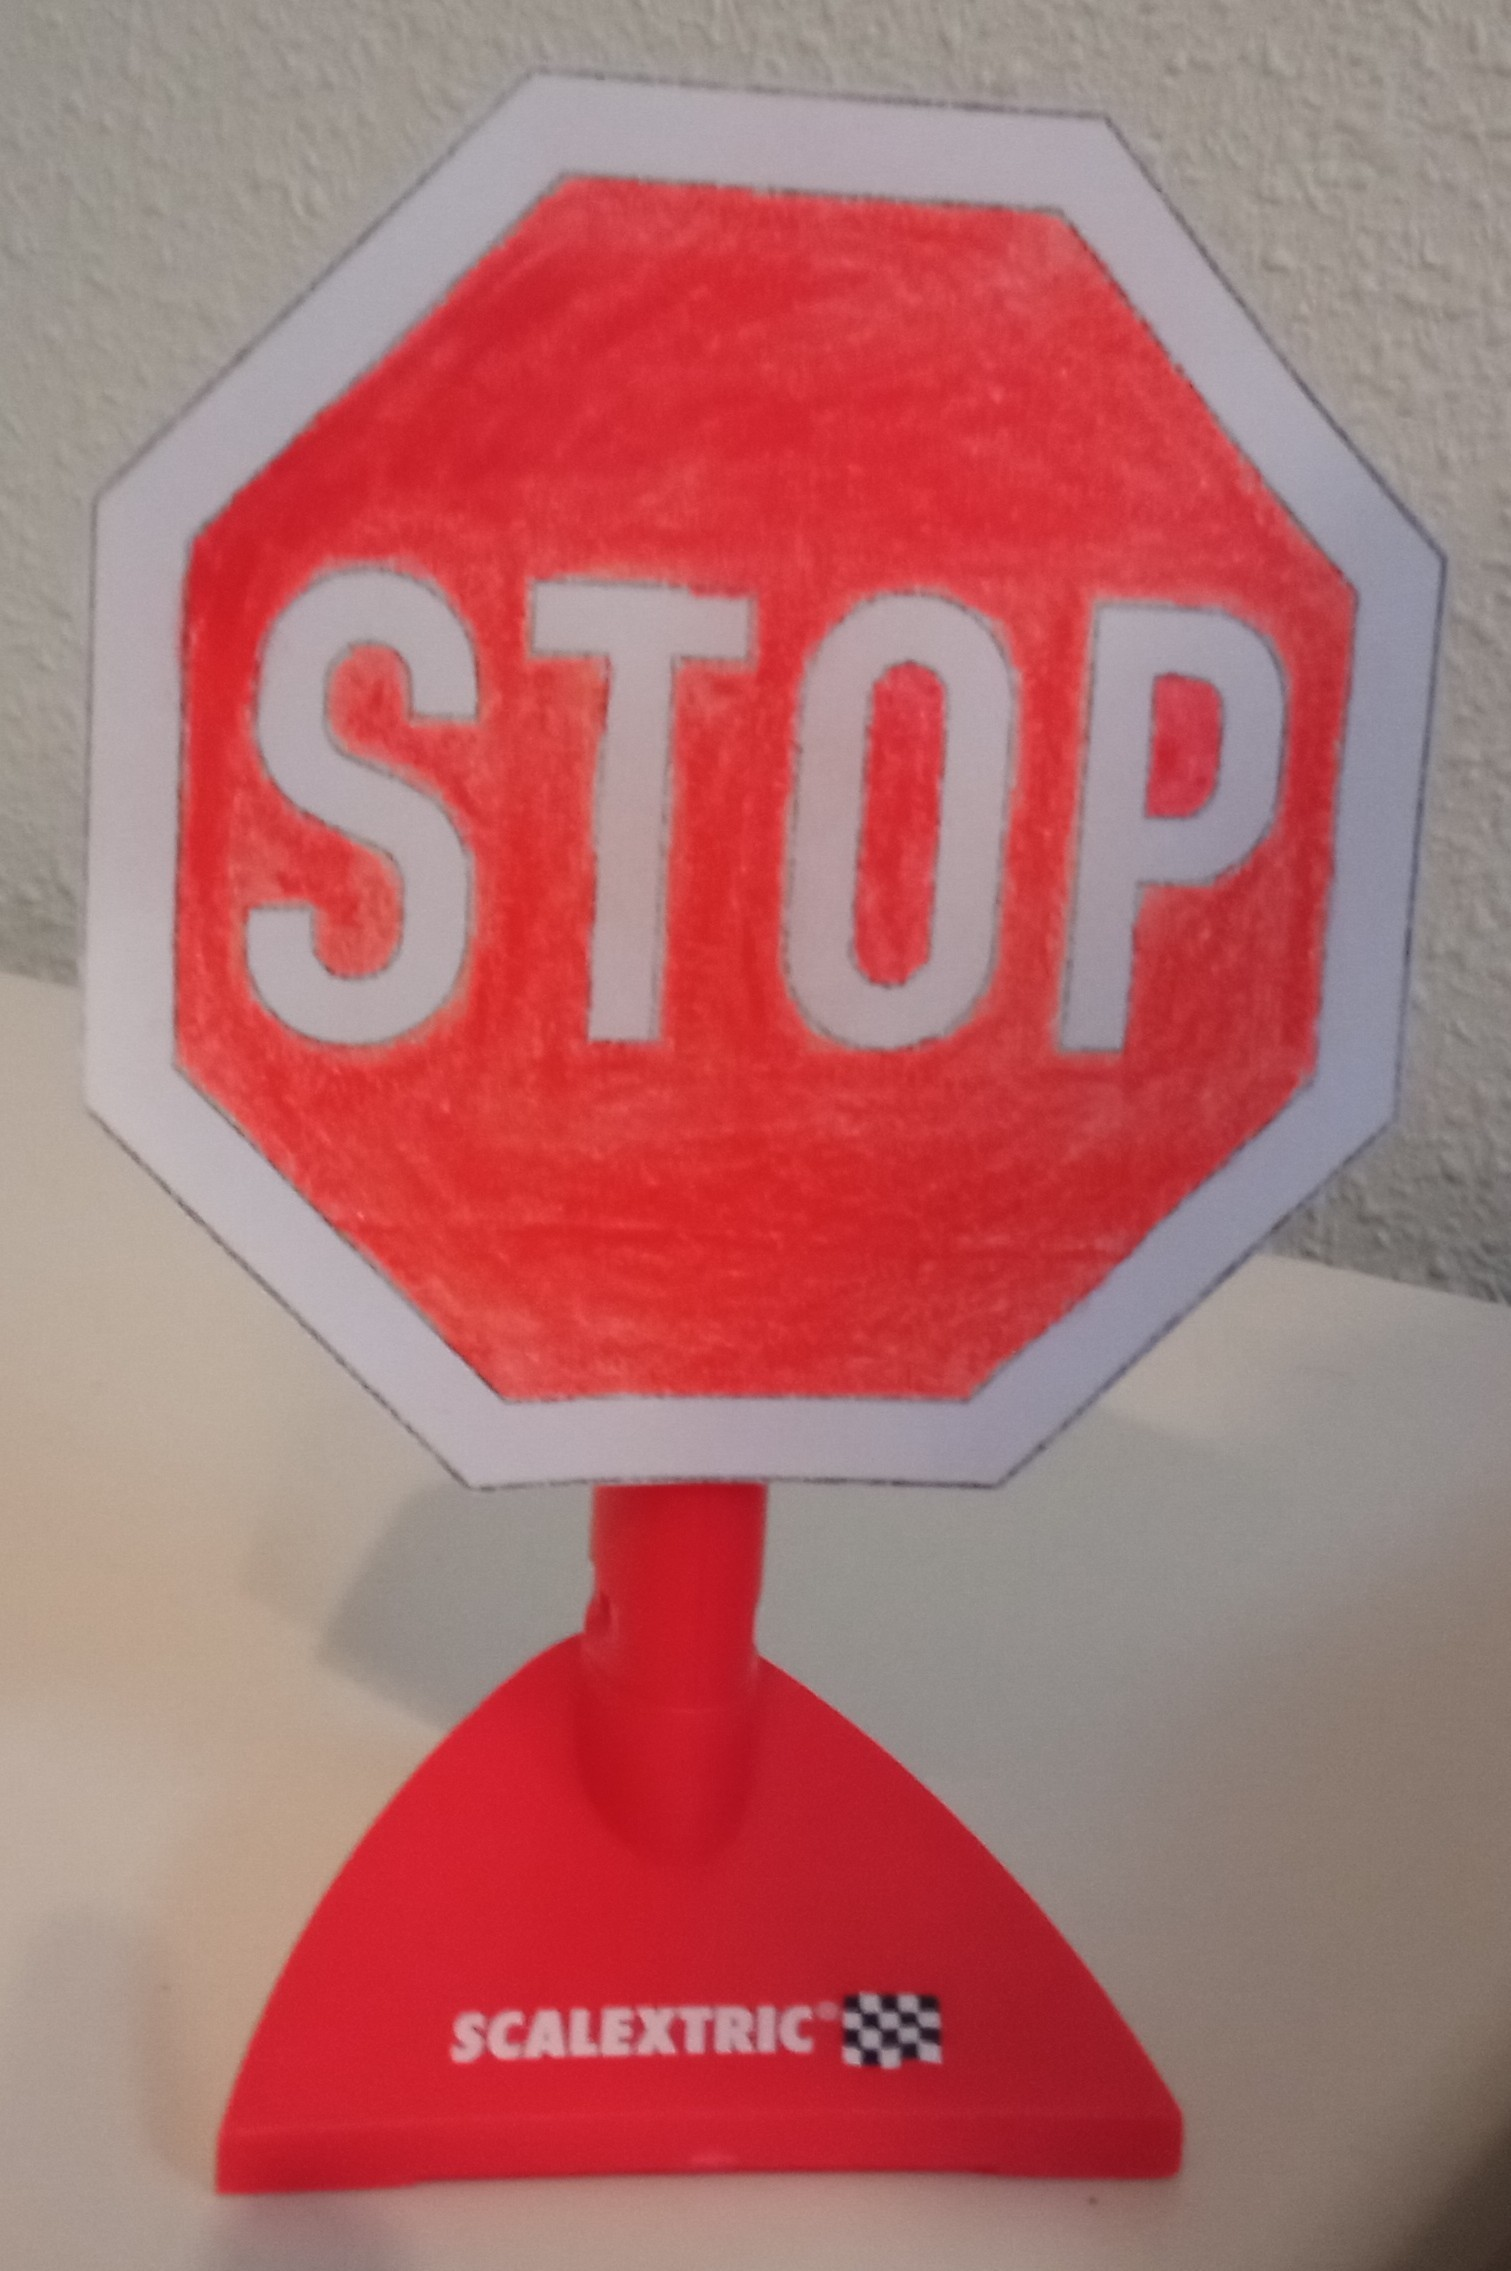
\includegraphics[width=4cm, height=5cm]{figs/realstopsign}\hspace{0.5cm}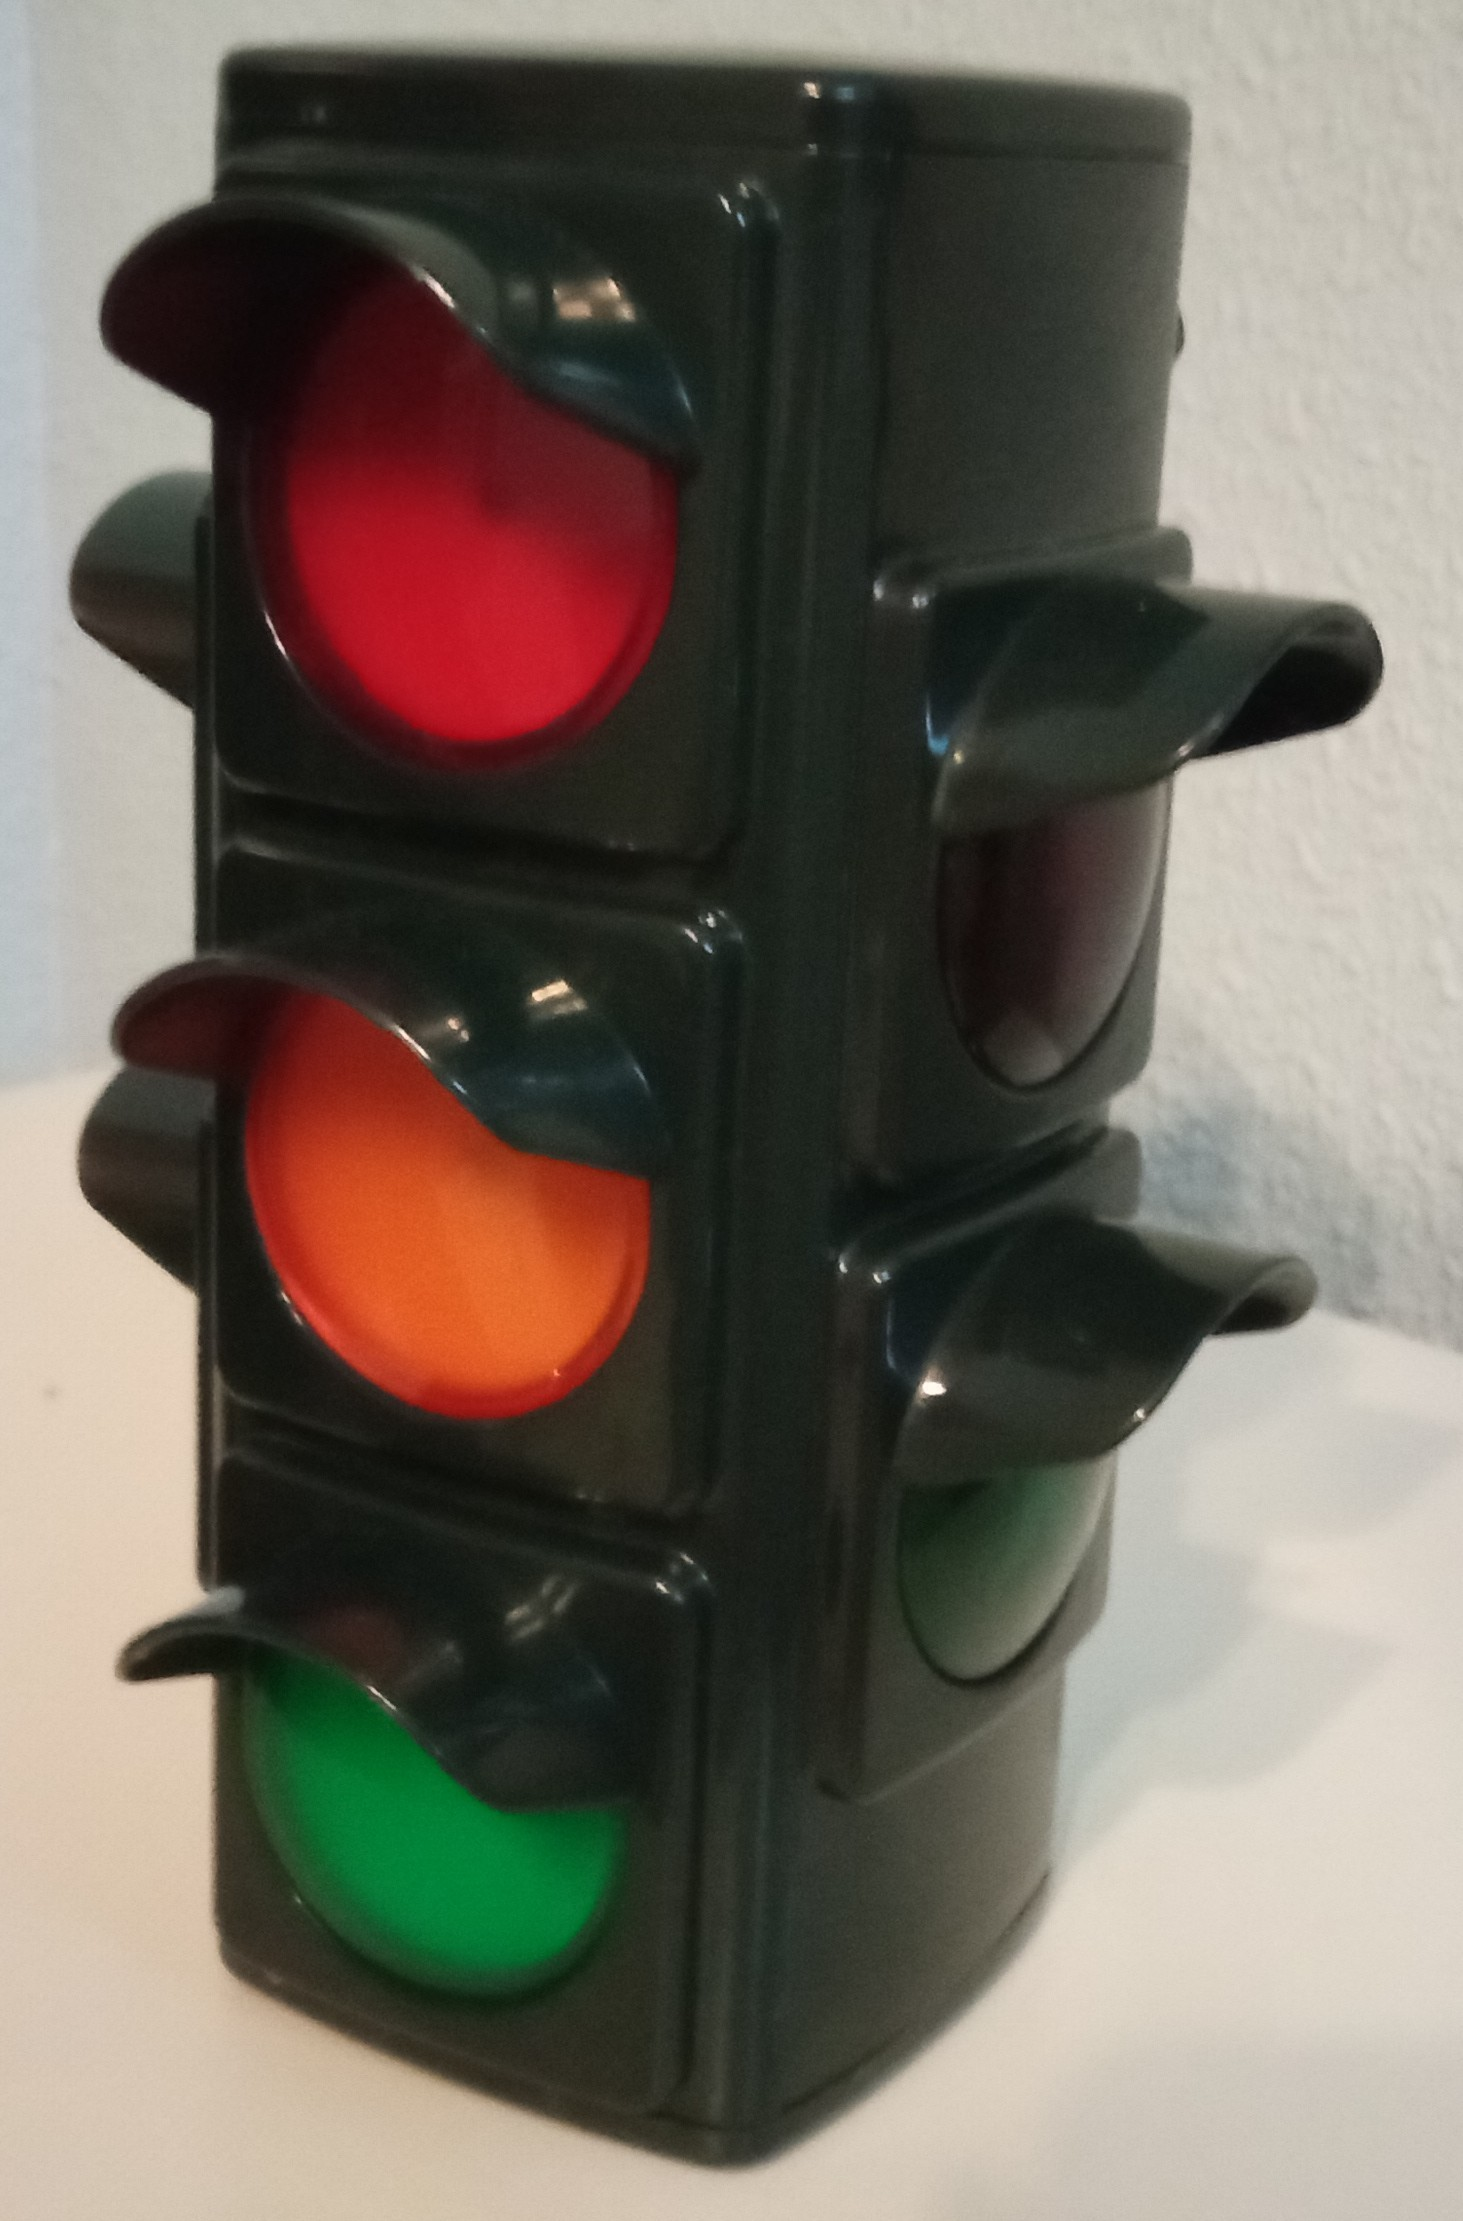
\includegraphics[width=4cm]{figs/realtrafficlight}\hspace{0.5cm}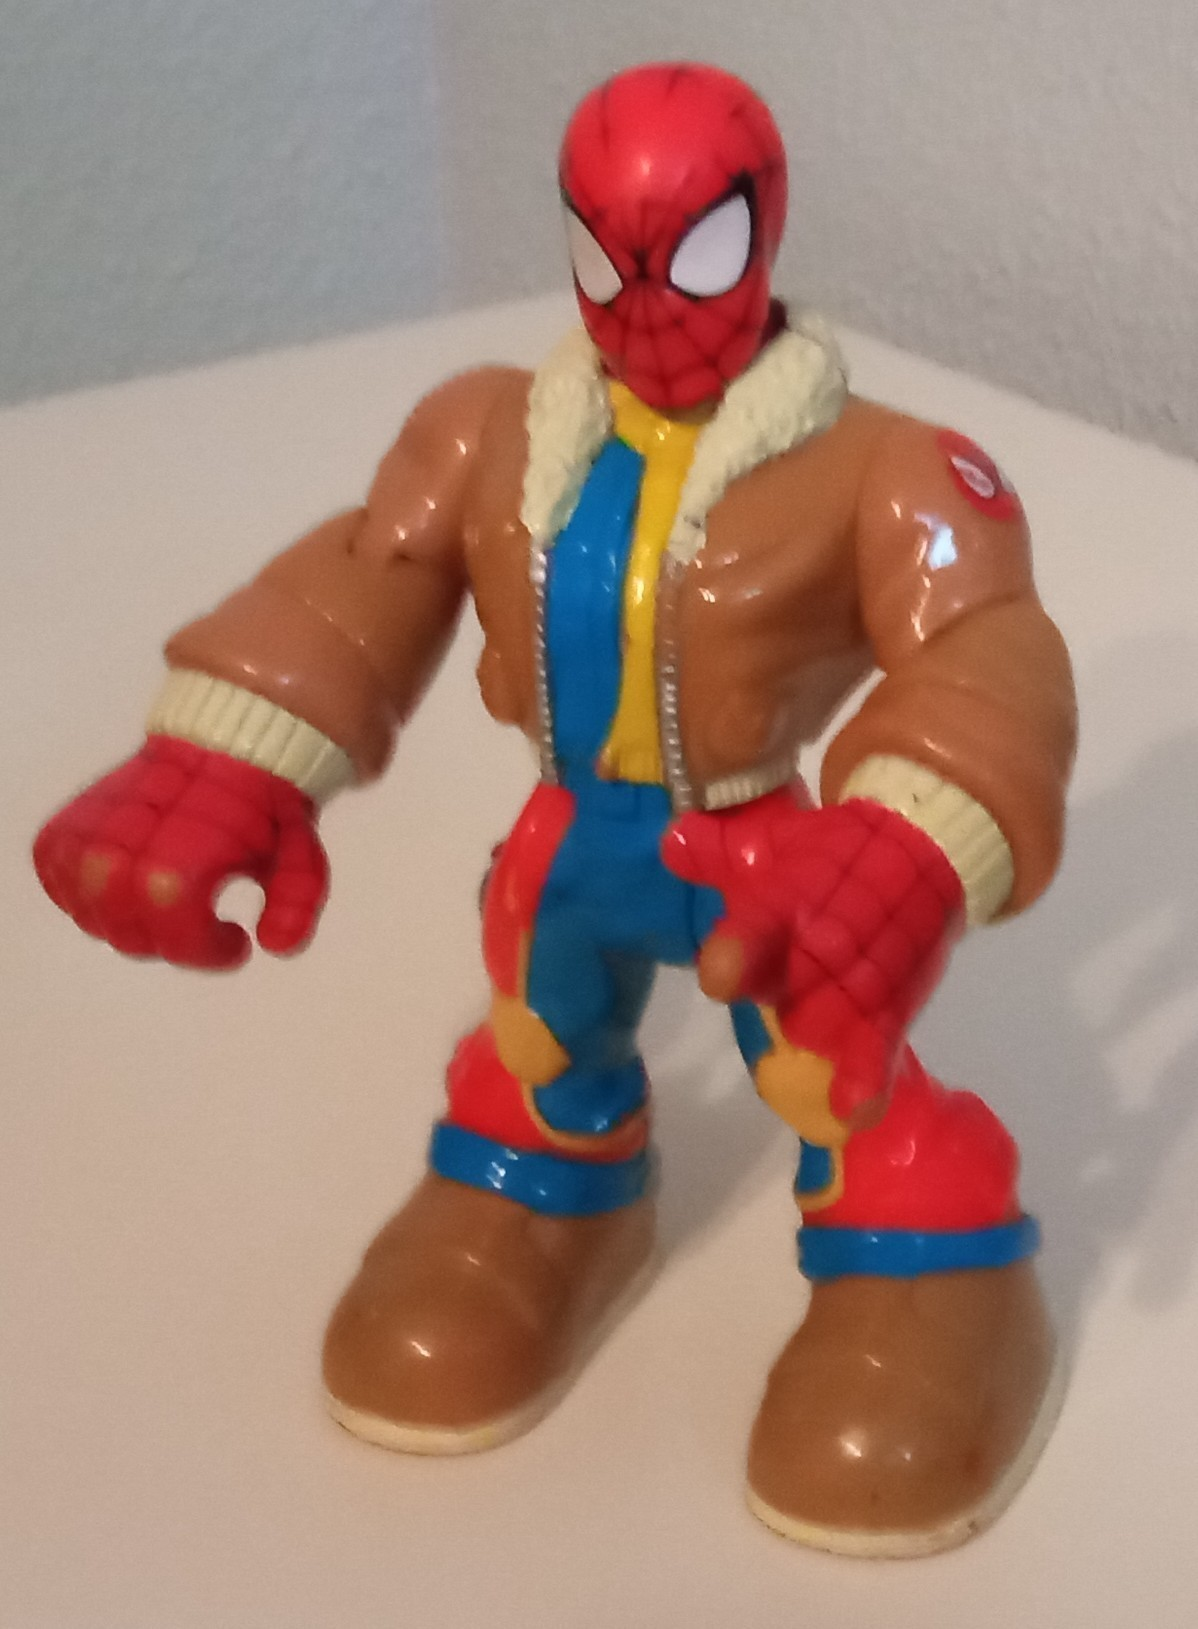
\includegraphics[width=4cm, height=5cm]{figs/realpedestrian}
	\end{center}
	\caption{Objetos reales dinámicos y estáticos.}
	\label{fig:objects}
\end{figure}\

\subsection{Circuito}
En principio se construyó un circuito inicial, representado en la Figura \ref{fig:circuit}, en el que se entrenó la red neuronal de seguimiento de carril. Posteriormente se fue agrandando en el espacio introduciendo rectas más largas para poder interactuar mejor con objetos.\\

\begin{figure} [h!]
	\begin{center}
		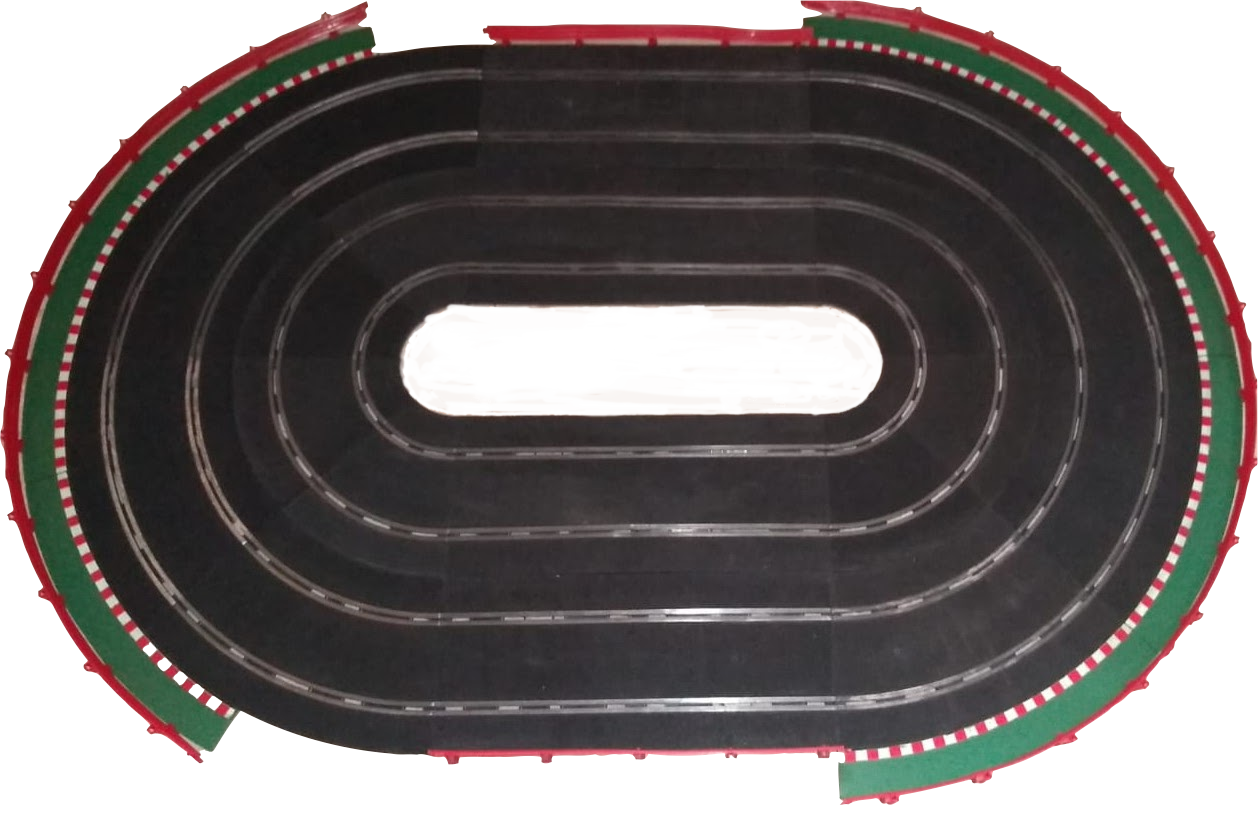
\includegraphics[width=8cm]{figs/circuit}
	\end{center}
	\caption{Circuito inicial construido a partir de pistas Scalextric.}
	\label{fig:circuit}
\end{figure}\

Tras ubicar todos los objetos alrededor del circuito, da como resultado la imagen representada en la Figura \ref{fig:circuitwithobjects}.\\

\begin{figure} [h!]
	\begin{center}
		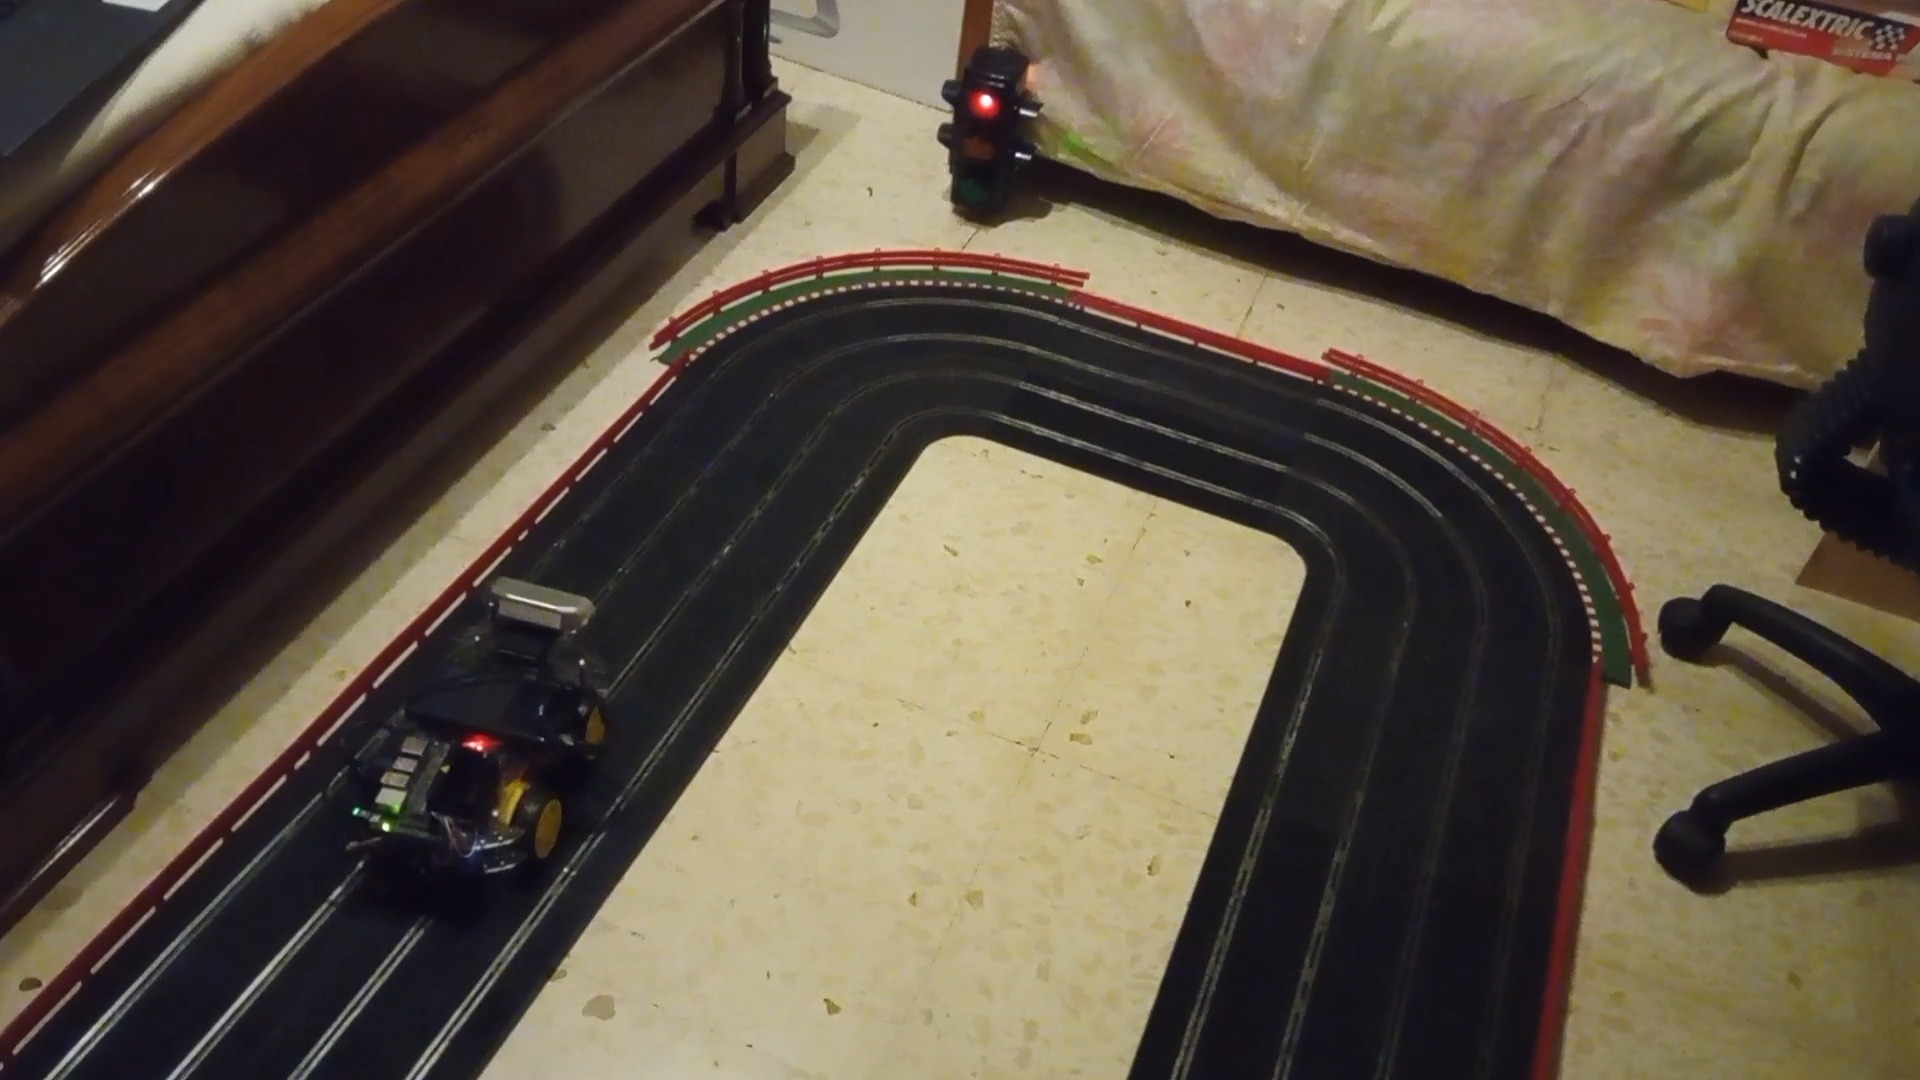
\includegraphics[width=12cm]{figs/circuitwithobjects}
	\end{center}
	\caption{Circuito con objetos.}
	\label{fig:circuitwithobjects}
\end{figure}\

\section{Redes neuronales en el entorno real}
El entrenamiento de la red neuronal \textit{ResNet-18} se realiza de igual forma que en el entorno simulado, la principal diferencia a tener en cuenta es la luz ambiente y los colores, que a diferencia del simulador, cambian dependiendo de como incida la luz. Por ello, es interesante comprobar el comportamiento de la red neuronal cuando hay cambios de luz. Además, existen multitud de diferencias entre una luz artificial y la luz natural, cuando se trabaja con luz natural es necesario tener en cuenta la incidencia que los rayos del sol pueden hacer sobre la lente de la cámara. Por ello se decidió entrenar la red con luz artificial, con imágenes como la que representa la Figura \ref{fig:imagedataset}, obteniendo el valor de 0.0034 como error. La librería \textit{JetRacer} recomienda entrenar la red con un mínimo de 50 imágenes\footnote{\url{https://github.com/NVIDIA-AI-IOT/jetracer/blob/master/docs/examples.md}}, por lo que se decidió entrenar con 100 imágenes para que el tiempo de entrenamiento no fuese demasiado elevado y no provocara un aumento muy grande de temperatura en la placa \textit{NVIDIA Jetson Nano}, que al no disponer de disipador activo, alcanza temperaturas muy elevadas.\\

\begin{figure} [h!]
	\begin{center}
		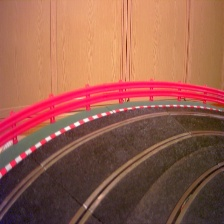
\includegraphics[width=4cm]{figs/imagedataset}\hspace{1cm}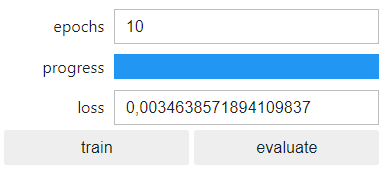
\includegraphics[width=6cm]{figs/epoch}
	\end{center}
	\caption{Imagen del \textit{dataset} utilizado entrenado con luz artificial y error al finalizar el entrenamiento.}
	\label{fig:imagedataset}
\end{figure}\

Una vez probada la red neuronal \textit{YOLO V3 Tiny} utilizada en el entorno simulado, se comprobó que era necesario bajar demasiado el límite o \textit{threshold} de detección, hasta 0.3, para poder detectar los objetos elegidos. A diferencia del entorno de simulación ,en el que dicho límite se fijó a 0.8. Esto provocaba falsos positivos y por tanto una detección poco fiable. Dicha circunstancia puede ser debida, entre otros motivos, a unos objetos reales algo distintos respecto a los que la red fue entrenada o una luz ambiental baja. Por ello se decidió entrenar la red con los objetos utilizados en el entorno real. Para ello, es necesario una tarjeta gráfica potente. Por lo que se realizó una comparativa entre las tarjetas gráficas disponibles para realizar el entrenamiento en el menor tiempo posible. Dicha comparativa está representada en el Cuadro \ref{table:versusnvidia}.\\

\begin{table}[H]
	\begin{center}
		\begin{tabular}{|c|c|c|c|c|}
			\hline
			\textbf{Placa}	& \textbf{Arquitectura} & \textbf{C.C\makebox[0pt][l]{$^*$}} & \textbf{GPU Cores}				& \textbf{RAM}
			\\
			\hline
			NVIDIA Jetson Nano		& Maxwell								& 5.3														& 128												& 4 GB
			\\
			NVIDIA MX330					& Pascal								& 6.1														& 384												& 2 GB
			\\
			NVIDIA AGX Xavier			& Volta									& 7.2														& 384 con 48 Tensor Cores		& 64 GB
			\\
			\hline
		\end{tabular}
		\parbox[t]{\textwidth}{\footnotesize C.C$^*$: capacidad de cómputo.}  
		\caption{Comparación entre las tarjetas gráficas disponibles para entrenar la red \textit{YOLO V3 Tiny}.}
		\label{table:versusnvidia}
	\end{center}
\end{table}

\subsection{Entrenamiento de la red \textit{YOLO V3 Tiny} para detección de objetos propios}
El objetivo es entrenar la red \textit{YOLO V3 Tiny} con el objetivo de poder detectar objetos propios o mejorar la probabilidad de detección de objetos ya detectados por la red.\\

Para ello, es pertinente saber qué \textit{dataset} se ha utilizado para generar los pesos actualmente usados. Atendiendo a la página oficial de \textit{YOLO\footnote{\url{https://pjreddie.com/darknet/yolo/}}}, el \textit{dataset} utilizado es \textit{COCO}. Por lo que será necesario obtener las imágenes y sus ficheros de etiquetado donde se asocian los objetos presentes en las imágenes. Existe un repositorio\footnote{\url{https://github.com/KaranJagtiani/YOLO-Coco-Dataset-Custom-Classes-Extractor}} que permite la extracción, a partir del \textit{dataset} mencionado, de las clases de objetos deseadas.\\

El formato del archivo de etiquetado de los objetos es muy relevante. El formato por defecto de \textit{COCO} es el contenido en el Código \ref{cod:formatcoco}\footnote{\url{https://cocodataset.org/\#format-data}}. Y el utilizado en \textit{YOLO} es el contenido en el Código \ref{cod:formatyolo}\footnote{\url{https://github.com/AlexeyAB/darknet\#how-to-train-to-detect-your-custom-objects}}. Por lo que es necesario realizar la conversión de un formato a otro. Este proceso también lo realiza el programa contenido en el repositorio anteriormente mencionado.\\

\begin{code}[h]
	\begin{lstlisting}
		annotation{
			"id": int, 
			"image_id": int, 
			"category_id": int, 
			"segmentation": RLE or [polygon], 
			"area": float, 
			"bbox": [x,y,width,height], 
			"iscrowd": 0 or 1,
		}

		categories[{
			"id": int, 
			"name": str, 
			"supercategory": str,
		}]
	\end{lstlisting}
	\caption[Formato de etiquetado de objetos utilizado por \textit{COCO}.]{Formato de etiquetado de objetos utilizado por \textit{COCO}.}
	\label{cod:formatcoco}
\end{code}

\begin{code}[h]
	\begin{lstlisting}
		<object-class> <x_center> <y_center> <width> <height>
	\end{lstlisting}
	\caption[Formato de etiquetado de objetos utilizado por \textit{YOLO}.]{Formato de etiquetado de objetos utilizado por \textit{YOLO}.}
	\label{cod:formatyolo}
\end{code}

Como se mencionó en el Capítulo 2, se ha utilizado la librería \textit{LabelIMG} para realizar el etiquetado de los objetos y generar el archivo en formato compatible con \textit{YOLO}. En la Figura \ref{fig:customlabelimg} se representa el etiquetado de uno de los objetos reales con dicha librería.\\

\begin{figure} [h!]
	\begin{center}
		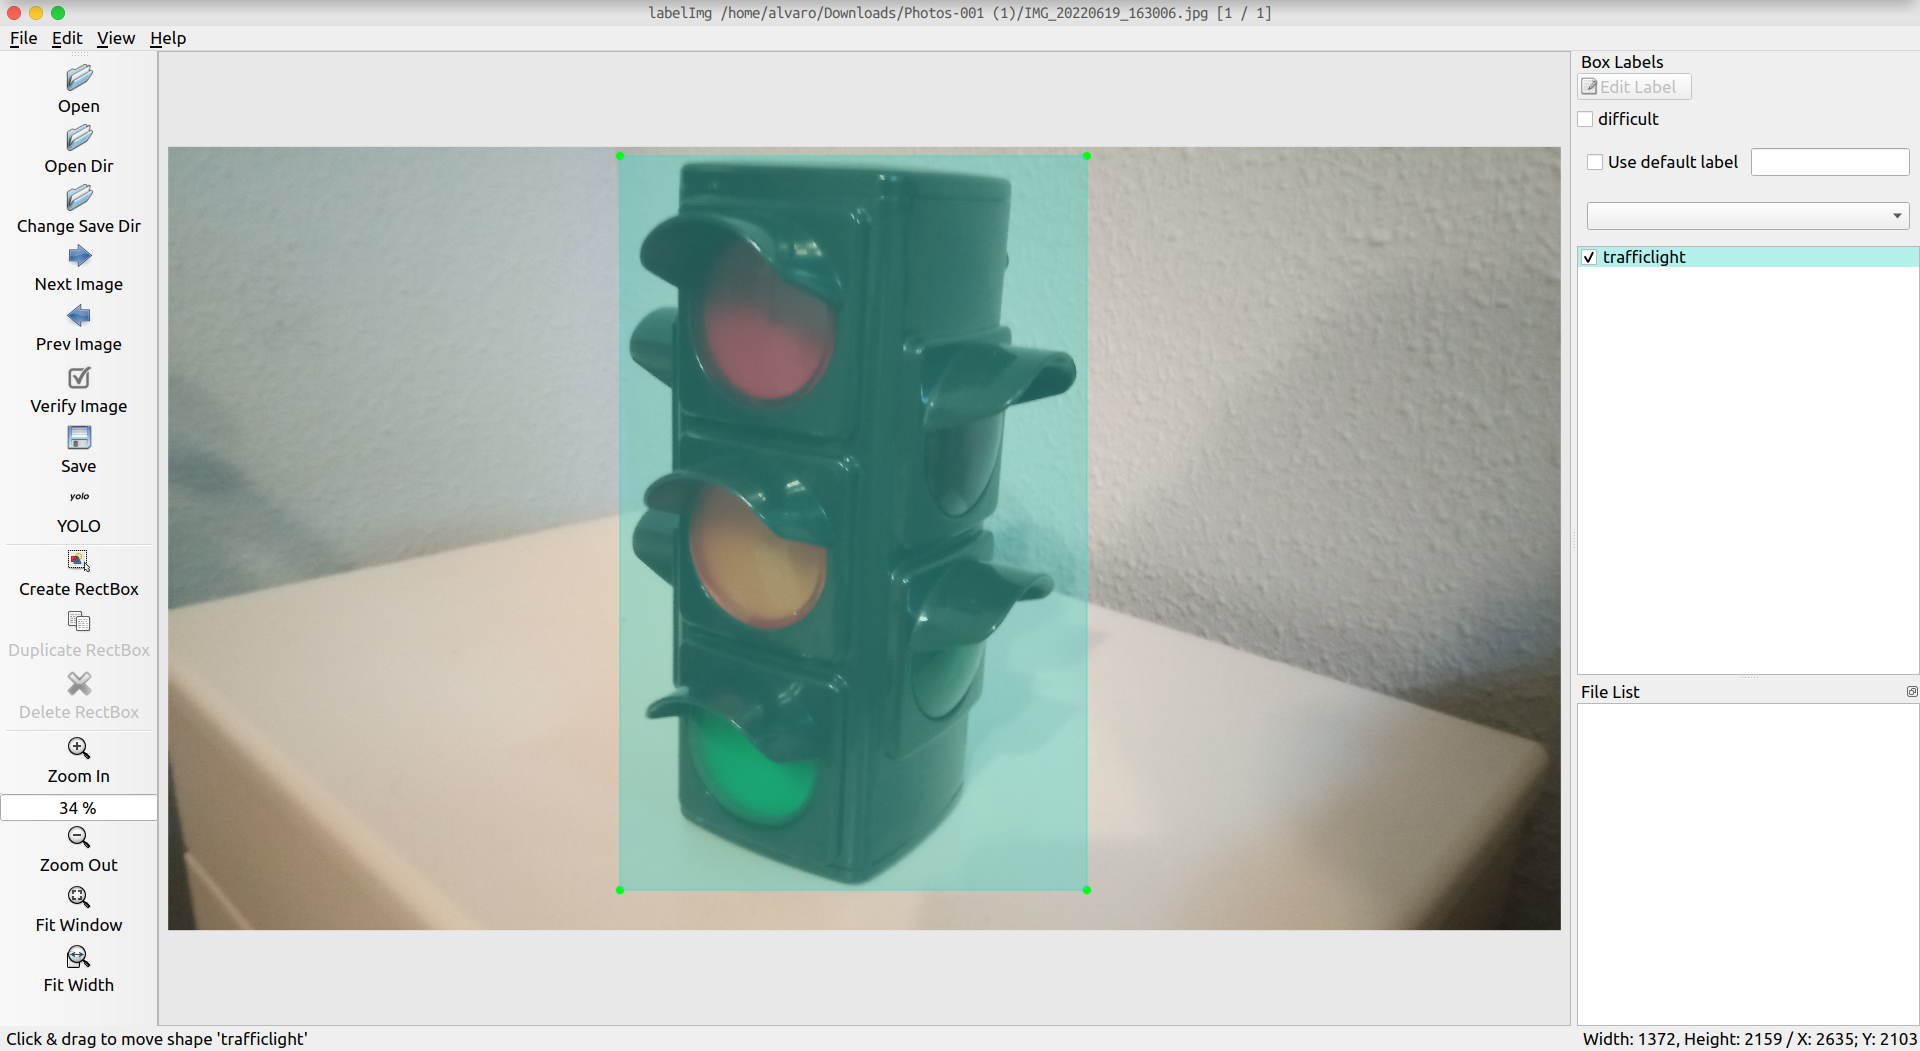
\includegraphics[width=12cm]{figs/customlabelimg}
	\end{center}
	\caption{Etiquetado de objetos propios con la herramienta \textit{LabelIMG}.}
	\label{fig:customlabelimg}
\end{figure}\

El gráfico representado en la Figura \ref{fig:graphcoco}, extraído de la siguiente fuente\cite{graphcoco}, muestra el número de imágenes de cada tipo de objeto. Se puede observar que el la clase persona está presente en imágenes, seis veces más que cualquier otro tipo de objeto. Esto se debe a que existen multitud de personas con distinto aspecto y por ello es necesario una cantidad muy grande de imágenes para obtener una detección fiable. Esto es determinante a la hora del entrenamiento, ya que al ser tan elevado el número de imágenes, el tiempo de entrenamiento será considerablemente grande.\\

\begin{figure} [h!]
	\begin{center}
		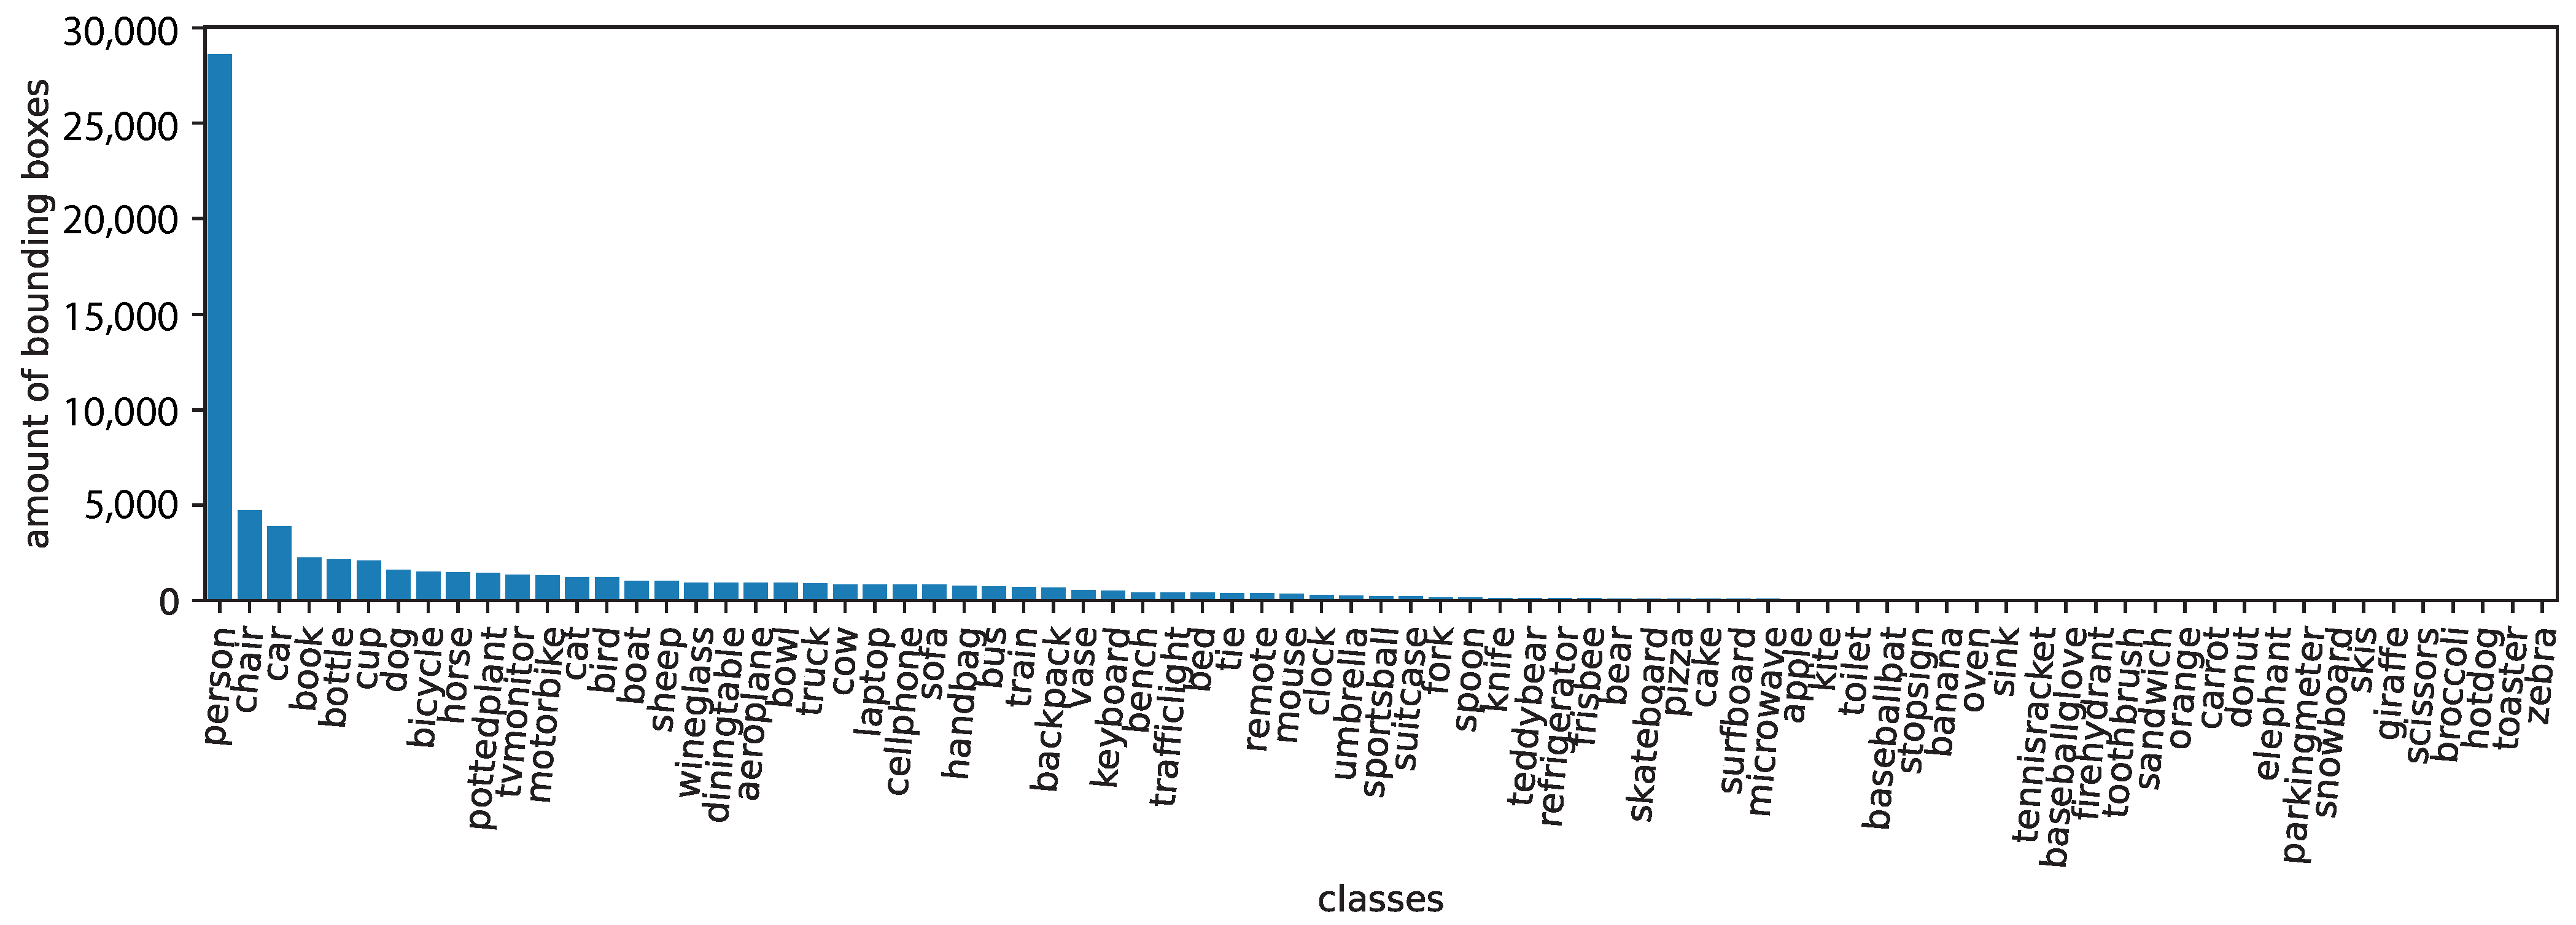
\includegraphics[width=14cm]{figs/graphcoco}
	\end{center}
	\caption{Distribución de las clases de objetos del \textit{dataset} COCO.}
	\label{fig:graphcoco}
\end{figure}\

Para proceder al entrenamiento, además del \textit{dataset} y sus ficheros de etiquetado, es necesario utilizar el \textit{framework} \textit{Darknet\footnote{\url{https://github.com/pjreddie/darknet}}} y hacer uso del comando \verb|partial| para obtener los pesos preentrenados sobre los cuales, se entrenará la red con el \textit{dataset} elegido.\\

También es necesario modificar una serie de archivos entre los que se encuentra el \textit{cfg} que contiene los parámetros de la red. Las principales modificaciones a realizar son las siguientes:
\begin{itemize}
	\item El número de \textit{batch} deberá ser 64
	\item El número de \textit{subdivisions} deberá ser 2
	\item El número de \textit{max\_batches} deberá ser el número de clases multiplicado por 2000. Y este número no debe ser inferior al número total de imágenes
	\item El número de \textit{steps} deberá ser fijado al 80\% y al 90\% de \textit{max\_batches}
	\item La anchura y altura de la imagen con la que entrena la red deberá ser como mínimo 416. En el caso de querer detectar objetos muy pequeños dicho parámetro deberá ser modificado a 608 o 832
	\item En cada parámetro \textit{[yolo]} el número de clases de objetos a detectar deberá ser fijado y el número de \textit{filters} deberá fijarse atendiendo a la siguiente fórmula: \textit{(classes + 5) x 3}
\end{itemize}\

Se deberán crear los ficheros \textit{train.txt} y \textit{test.txt} donde deben estar las rutas absolutas a cada fichero de etiquetado. Y otro fichero llamado \textit{obj.data} que contenga las rutas de los archivos anteriormente descritos, dicho contenido está presente en el Código \ref{cod:objdata}.\\

\begin{code}[h]
	\begin{lstlisting}
		classes = 9
		train  = data/train.txt
		valid  = data/test.txt
		names = data/obj.names
		backup = backup/
	\end{lstlisting}
	\caption[Contenido del archivo \textit{obj.data} con las rutas de los archivos necesarios.]{Contenido del archivo \textit{obj.data} con las rutas de los archivos necesarios.}
	\label{cod:objdata}
\end{code}

Otro factor importante es el porcentaje de imágenes con el que no se entrena la red pero sí prueba para comprobar la validez de la misma. Estas imágenes componen el \textit{dataset} de validación y debe estar compuesto por un 20\% de las imágenes totales del \textit{dataset}.\\

Durante el entrenamiento se irá mostrando una gráfica que indica el progreso, representada en la Figura \ref{fig:chart}. En dicha gráfica se muestra el error de la red, se puede observar que el error final tras terminar el entrenamiento es de 0.663. Atendiendo a la guía\footnote{\url{https://github.com/AlexeyAB/darknet\#how-to-train-to-detect-your-custom-objects}} utilizada para entrenar la red, el error deberá estar entre 0.05 en el caso de un \textit{dataset} pequeño y simple a 3.0 en el caso de un \textit{dataset} grande y difícil, como es el caso de la clase persona.\\

\begin{figure} [h!]
	\begin{center}
		\includegraphics[width=12cm]{figs/chart}
	\end{center}
	\caption{Gráfica de entrenamiento mostrando el error de la red \textit{YOLO V3 Tiny}.}
	\label{fig:chart}
\end{figure}\

\subsection{Controlador diseñado para el seguimiento de carril a partir de la salida de la red neuronal}
Una vez obtenida la salida de la red neuronal que indica el centro del carril, es necesario elaborar un controlador que comande velocidades lineales y angulares al robot. Para ello se ha realizado un controlador proporcional (P) con una serie de constantes para lograr un comportamiento adecuado, dicho controlador está disponible en el Código \ref{cod:controller}.\\ 

\begin{code}[h]
	\begin{lstlisting}[language=Python]
		def setSteering(self, steering):
			if steering > self.FORWARD_RANGE:
				rightSpeed = self.STEERING_OFFSET + abs(steering * self.STEERING_GAIN)
				if rightSpeed < self.MIN_SPEED:
					rightSpeed = self.MIN_SPEED
				leftSpeed = self.TURNING_SPEED
				self.goRight()
			elif steering < -self.FORWARD_RANGE:
				leftSpeed = self.STEERING_OFFSET + abs(steering * self.STEERING_GAIN)
				if leftSpeed < self.MIN_SPEED:
					leftSpeed = self.MIN_SPEED
				rightSpeed = self.TURNING_SPEED
				self.goLeft()
			else:
				self.goForward()
				leftSpeed = self.throttleMotor
				rightSpeed = self.throttleMotor
			
			self.setSpeed(leftSpeed, rightSpeed)
	\end{lstlisting}
	\caption[Controlador P realizado para el seguimiento de carril.]{Controlador P realizado para el seguimiento de carril.}
	\label{cod:controller}
\end{code}

\subsection{Transformación del modelo de \textit{PyTorch a TensorRT}}
Como se expuso en el Capítulo 3, existe una librería llamada \textit{PyTorch to TensorRT} capaz de convertir modelos de \textit{PyTorch} a modelos optimizados aprovechando los tensores de las gráficas dedicadas, si bien la placa \textit{NVIDIA Jetson Nano} no dispone de una GPU con tensores\footnote{\url{https://connecttech.com/jetson/jetson-module-comparison/}}, sí permite realizar inferencia utilizando operaciones con \textit{FP16} lo que aumenta el rendimiento en gran medida. Esta conversión se realiza de forma muy sencilla llamando a la función \verb|torch2trt()| tal y como representa el Código \ref{cod:torch2trt}.\\

\begin{code}[h]
	\begin{lstlisting}[language=Python]
		data = torch.zeros((1, 3, 224, 224)).cuda().half()
		model_trt = torch2trt(model, [data], fp16_mode=True)
		torch.save(model_trt.state_dict(), 'model_tensor.pth')
	\end{lstlisting}
	\caption[Conversión del modelo para realizar optimización y aumentar el rendimiento.]{Conversión del modelo para realizar optimización y aumentar el rendimiento.}
	\label{cod:torch2trt}
\end{code}

En la Figura \ref{fig:screenshotsreal} están representadas capturas de la ejecución en el entorno real desde la perspectiva de la visión del robot.\\

\begin{figure} [h!]
	\begin{center}
		\includegraphics[width=6cm]{figs/screenshottrafficlight}\hspace{0.5cm}\includegraphics[width=6cm]{figs/screenshotstopsign}
	\end{center}
	\caption{Visión del robot durante la ejecución en el entorno real.}
	\label{fig:screenshotsreal}
\end{figure}\

\section{Diseño del software a partir de un diagrama de clases}
El diseño del software se ha realizado a partir de un diagrama de clases, utilizando la herramienta \textit{UMLET\footnote{\url{hhttps://www.umlet.com/}}}, que permite estructurar crear clases, dependencias entre ellas y los atributos y funciones que contiene. El presente diseño, representado en la Figura \ref{fig:diagram}, contiene una clase principal llamada \textit{AutonomousVehicle} que tiene instancias de la clase \textit{LaneFollower} que implementa el seguimiento de carril, de la clase \textit{JetRacer} que implementa el controlador del vehículo y la comunicación con los motores del mismo. También contiene una instancia de la clase \textit{ObjectDetector} que implementa la detección de objetos y, a su vez, la clase \textit{ObjectDetector} hace uso del flujo de vídeo proveniente de un \textit{topic} de \textit{ROS}.\\

\begin{figure} [h!]
	\begin{center}
		\includegraphics[width=14cm]{figs/diagram5}
	\end{center}
	\caption{Diagrama de clases.}
	\label{fig:diagram}
\end{figure}\

% Tabla cámara
% Buscar ....
% Gráfica entrenamiento error no sube ni baja, estable carril
% Resnet
% NN siempre yxy?
% .yaml stop or stop sign?
% Tesnor cores
% yolov3-tiny.conv.15 15 convolución 15
% singlestone
% \textit{Over-fitting}
% muestra el número de imágenes??????? y causas
% Salir de sección screenshotsreal


\chapter{Conclusiones}
\label{cap:capitulo5}
En este capítulo se realiza un resumen de los problemas resueltos y las soluciones utilizadas, así como los experimentos realizados para validar los resultados. Por último, se citan una serie de posibles usos alternativos del software utilizado.

\section{Conclusiones}
\label{section:conclusiones}
El objetivo principal de este trabajo era implementar un coche autónomo bajo una plataforma de bajo coste y reducido tamaño, capaz de circular por un circuito o carretera en un entorno dinámico interactuando con objetos propios de una ciudad, como semáforos, señales de stop o peatones. Dicho objetivo debía ser llevado a cabo en dos entornos distintos; en un entorno simulado, utilizando el simulador \textit{Gazebo}\footnote{\url{https://github.com/gazebosim/gz-sim}}, y en un entorno real, ensamblando un robot donde se utiliza como cerebro una placa de desarrollo \textit{NVIDIA Jetson Nano}\footnote{\url{https://developer.nvidia.com/embedded/jetson-nano}} y, como sensor principal, una cámara USB.\\

Dichos objetivos se han cumplido satisfactoriamente; para ello se han utilizado dos redes neuronales. Por un lado, para realizar el seguimiento de carril, se ha hecho uso de la librería \textit{JetRacer}\footnote{\url{https://github.com/NVIDIA-AI-IOT/jetracer}}. Dicha librería implementa una red residual, concretamente la red preentrenada \textit{ResNet-18}, que mediante un entrenamiento previo a partir de un \textit{dataset} propio, proporciona como salida de la red, el centro del carril o carretera. Dicha salida se utiliza como entrada en un controlador implementado para poder seguir recto o girar en caso de enfrentarse a una curva. Cabe destacar que este método no tiene como requisito un mapa del entorno, por lo que resulta útil cuando no se dispone del mismo o se quiere seguir una ruta de forma más precisa.\\

Por otro lado, se ha utilizado la red \textit{YOLO V3 Tiny} mediante el \textit{framework} \textit{Darknet}\footnote{\url{https://pjreddie.com/darknet/}} y su implementación en \textit{ROS}, \textit{Darknet ROS}, para la detección de objetos. En el caso del entorno real, la red mencionada ha sido entrenada a través de un \textit{dataset} propio con los objetos reales, con el objetivo de ofrecer una detección de mayor fiabilidad. 
Todo ello ha sido combinado en dos paquetes \textit{ROS}, diferenciando entorno simulado y real.\\

La principal limitación del sistema es la potencia de la placa utilizada. Al necesitar dos redes neuronales, y para obtener un rendimiento aceptable, es necesario trabajar con una resolución considerablemente baja. Por otra parte, al disponer de una sola cámara, esta debe tener un determinado ángulo de inclinación hacia abajo para poder visualizar correctamente el circuito, lo que provoca un campo de visión reducido que limita la detección de objetos de gran altura.

\section{Líneas futuras}
\label{section:future}
Tal y como se expuso en el Capítulo \ref{cap:capitulo1}, existen multitud de casos donde se utilizan vehículos autónomos, y no únicamente en el ámbito de la conducción. Por lo que la solución implementada podría ser aplicable a otros usos. Por ejemplo, en el ámbito de la inspección, la red neuronal de seguimiento de carril podría ser utilizada para navegar a lo largo de un túnel, como el de la Figura \ref{fig:moreusages}, en el que buscan artefactos explosivos a través de la red de detección de objetos.\\

Otra posible utilidad sería la exploración de bosques o montañas para prevenir incendios, de modo que el robot debería seguir la senda o camino en busca de fuego o realizando tareas de prevención, haciendo uso de la detección de objetos para poder alertar correctamente.

\begin{figure} [h!]
	\begin{center}
		\includegraphics[width=6cm]{figs/tunel}\hspace{0.5cm}\includegraphics[width=6cm]{figs/forest}
	\end{center}
	\caption{Posibles usos alternativos del software implementado.}
	\label{fig:moreusages}
\end{figure}\

Todo ello son ámbitos de aplicación que no hacen más que proporcionar una intuición acerca del potencial de las redes neuronales que, mediante un entrenamiento a través de un conjunto grande y completo de datos, permiten adaptarse a multitud de situaciones.\\

% que es red preentrenada
% real time
% parameter width from calculated path

\clearpage
\thispagestyle{empty}

\printindex \nocite{*}
\appendix
\bibliographystyle{apalike} \bibliography{bibliografia}

\end{document}
